\documentclass[
    headings=optiontotocandhead,% Erweiterung für das optionale Argument der
                                % Gliederungsbefehle aktiviert.
    oneside,
    numbers=noenddot,% Keine Punkte am Ende der Gliederungsnummern und davon
                     % abgeleiteten Nummern
    toc= %Flache TOC
    12pt, % Schriftgröße 
    titlepage, % es wird eine Titelseite verwendet 
    parskip=false, % Abstand zwischen Absätzen (ganze Zeile) 
    listof=totoc, % Verzeichnisse im Inhaltsverzeichnis aufführen 
    listof=flat, % mehr Abstand für grosse Zahlen
    numbers=noenddot, % kein Punkt am Ende bei N7ummern 
    %%enlargefirstpage,% Gibt es bei scrartcl nicht!!!!
    bibliography=totoc, % Literaturverzeichnis im Inhaltsverzeichnis aufführen 
    %index=totoc, % Index im Inhaltsverzeichnis aufführen 
    %captions=tableheading, % Beschriftung von Tabellen für Ausgabe oberhalb
                           % der Tabelle formatieren 
    %draft % Status des Dokuments (final/draft) draft hinzufügen zum anziegen 
	%%der zeilen ende
    a4paper,DIV=14,
    BCOR=15mm,
    % captions=tablesignature,
]{scrbook}

\setcounter{secnumdepth}{3}

\usepackage[T1]{fontenc}
\usepackage[utf8]{inputenc}

\usepackage[english, ngerman]{babel} % your native language must be the last one!!

\usepackage{lastpage}
\usepackage{listings}
\usepackage{blindtext}

%% Aufzählungen nicht so weit einrücken
\usepackage[inline]{enumitem}
%\setitemize{leftmargin=*} 
% Listen etwas wenige einrücken, erfordert enumitem
\setitemize{leftmargin=*}

\usepackage{lmodern}

\usepackage{xspace}

\usepackage{graphicx}

\usepackage{chngcntr}

%%? \usepackage{textcomp}
\usepackage[hyphens]{url}
\usepackage{makeidx}
\makeindex
%%? \usepackage{graphicx}
\usepackage[numbers]{natbib}
\PassOptionsToPackage{normalem}{ulem}
\usepackage{ulem}

\usepackage{needspace}

\setlength\partopsep{0.5ex}%schoenere Listen
\usepackage[bottom]{footmisc}%fussnote ganz unten

\usepackage[]{microtype}
\UseMicrotypeSet[protrusion]{basicmath} % disable protrusion for tt fonts

\usepackage{multirow}   % Allows table elements to span several rows.
\usepackage{booktabs}   % Improves the typesettings of tables.
\usepackage{subcaption} % Allows the use of subfigures and enables their referencing.
\usepackage[ruled,linesnumbered,algochapter]{algorithm2e} % Enables the writing of pseudo code.
\usepackage[usenames,dvipsnames,table]{xcolor} % Allows the definition and use of colors. This package has to be included before tikz.
\usepackage{nag}       % Issues warnings when best practices in writing LaTeX documents are violated.
\usepackage{todonotes} % Provides tooltip-like todo notes.
\usepackage{float}
\usepackage{color}

%% bessere Suche im PDF
\input{glyphtounicode}
\pdfgentounicode=1
%%%%%%%%%%%%%%%%%%%%%%%%%%%%%%%%%%%%%%%%%%%%%%%%%%%%%%%%%%%%%%%%%%%%%%%%%%%%%%%%%%

%  Kopf und Fußzeilen -- links und rechts verschieden 
\newcommand{\kopfseitenummer}{{\bfseries \thepage}}
\newcommand{\kopfkapl}{{\bfseries\leftmark}}
\newcommand{\kopfkapr}{{\bfseries\rightmark}}
\newcommand{\kopfbild}{\voffset7mm
\includegraphics[width=25mm]{HTL3RLogoRGB}}
\newcommand{\kopfHTL}{Höhere Technische Bundeslehranstalt Wien 3, \\Rennweg 	Abteilung für Informationstechnologie}

\usepackage[automark,headsepline,footsepline,plainfootsepline]{scrlayer-scrpage}
%\automark[chapter]{chapter}% Eventuell wenn doppelseitig
\setkomafont{pageheadfoot}{\normalcolor\footnotesize\scshape}
\setkomafont{pagenumber}{\normalfont\normalsize}
\clearpairofpagestyles
\ihead{\headmark}
\ohead{\kopfbild}
\ifoot{\kapitelautor}
\ofoot{\pagemark}
\ModifyLayer[addvoffset=-.6ex]{scrheadings.foot.above.line}% Linie verschieben
\ModifyLayer[addvoffset=-.6ex]{plain.scrheadings.foot.above.line}% Linie verschieben
\setlength{\headheight}{32pt}

% alle Seiten mit Kopfzeile
\renewcommand{\chapterpagestyle}{scrheadings}

%% Kapitel - aufwändige Kapitelüberschriften
%Options: Sonny, Lenny, Glenn, Conny, Rejne, Bjarne, Bjornstrup
%\usepackage[Bjornstrup]{fncychap}
% Alternative: 
%\usepackage{titlesec}

% Verzeichnisse - aufwändiger
%\usepackage{tocloft}


%% Code Beispiele
%% eine Variante 
\usepackage{listings}
\renewcommand{\lstlistingname}{\inputencoding{utf8}Listing}
%% andere Variante
%\usepackage{minted}
%\setminted{
%  linenos,
%  frame=lines,
%  framesep=2mm,
%  breaklines=true
%}
% Beispiel
%\begin{listing}[H]
%\begin{minted}{bash}
%...
%\end{minted}
%\caption{Beschreibung}
%\end{listing}
%% dritte Variante 
% mit/für pandoc
% create
% pandoc -s sample.md -o sample.tex
% -> copy/paste

\usepackage{fancyvrb}
\newcommand{\VerbBar}{|}
\newcommand{\VERB}{\Verb[commandchars=\\\{\}]}
\DefineVerbatimEnvironment{Highlighting}{Verbatim}{commandchars=\\\{\}}
% Add ',fontsize=\small' for more characters per line
\newenvironment{Shaded}{}{}
\newcommand{\KeywordTok}[1]{\textcolor[rgb]{0.00,0.44,0.13}{\textbf{#1}}}
\newcommand{\DataTypeTok}[1]{\textcolor[rgb]{0.56,0.13,0.00}{#1}}
\newcommand{\DecValTok}[1]{\textcolor[rgb]{0.25,0.63,0.44}{#1}}
\newcommand{\BaseNTok}[1]{\textcolor[rgb]{0.25,0.63,0.44}{#1}}
\newcommand{\FloatTok}[1]{\textcolor[rgb]{0.25,0.63,0.44}{#1}}
\newcommand{\ConstantTok}[1]{\textcolor[rgb]{0.53,0.00,0.00}{#1}}
\newcommand{\CharTok}[1]{\textcolor[rgb]{0.25,0.44,0.63}{#1}}
\newcommand{\SpecialCharTok}[1]{\textcolor[rgb]{0.25,0.44,0.63}{#1}}
\newcommand{\StringTok}[1]{\textcolor[rgb]{0.25,0.44,0.63}{#1}}
\newcommand{\VerbatimStringTok}[1]{\textcolor[rgb]{0.25,0.44,0.63}{#1}}
\newcommand{\SpecialStringTok}[1]{\textcolor[rgb]{0.73,0.40,0.53}{#1}}
\newcommand{\ImportTok}[1]{#1}
\newcommand{\CommentTok}[1]{\textcolor[rgb]{0.38,0.63,0.69}{\textit{#1}}}
\newcommand{\DocumentationTok}[1]{\textcolor[rgb]{0.73,0.13,0.13}{\textit{#1}}}
\newcommand{\AnnotationTok}[1]{\textcolor[rgb]{0.38,0.63,0.69}{\textbf{\textit{#1}}}}
\newcommand{\CommentVarTok}[1]{\textcolor[rgb]{0.38,0.63,0.69}{\textbf{\textit{#1}}}}
\newcommand{\OtherTok}[1]{\textcolor[rgb]{0.00,0.44,0.13}{#1}}
\newcommand{\FunctionTok}[1]{\textcolor[rgb]{0.02,0.16,0.49}{#1}}
\newcommand{\VariableTok}[1]{\textcolor[rgb]{0.10,0.09,0.49}{#1}}
\newcommand{\ControlFlowTok}[1]{\textcolor[rgb]{0.00,0.44,0.13}{\textbf{#1}}}
\newcommand{\OperatorTok}[1]{\textcolor[rgb]{0.40,0.40,0.40}{#1}}
\newcommand{\BuiltInTok}[1]{#1}
\newcommand{\ExtensionTok}[1]{#1}
\newcommand{\PreprocessorTok}[1]{\textcolor[rgb]{0.74,0.48,0.00}{#1}}
\newcommand{\AttributeTok}[1]{\textcolor[rgb]{0.49,0.56,0.16}{#1}}
\newcommand{\RegionMarkerTok}[1]{#1}
\newcommand{\InformationTok}[1]{\textcolor[rgb]{0.38,0.63,0.69}{\textbf{\textit{#1}}}}
\newcommand{\WarningTok}[1]{\textcolor[rgb]{0.38,0.63,0.69}{\textbf{\textit{#1}}}}
\newcommand{\AlertTok}[1]{\textcolor[rgb]{1.00,0.00,0.00}{\textbf{#1}}}
\newcommand{\ErrorTok}[1]{\textcolor[rgb]{1.00,0.00,0.00}{\textbf{#1}}}
\newcommand{\NormalTok}[1]{#1}


%% should be last packages
\usepackage{scrhack}

\usepackage[unicode=true,
 bookmarks=true,bookmarksnumbered=false,bookmarksopen=false,
 breaklinks=true,pdfborder={0 0 0},backref=false,colorlinks=false]
 {hyperref}
\hypersetup{pdftitle={Insight},
 pdfauthor={Hatice Akyokus},
 pdfsubject={Diplomarbeit},
 pdfkeywords={dies, das}}
\urlstyle{same} % don't use monospace font for urls

%% for pandoc
\providecommand{\tightlist}{%
  \setlength{\itemsep}{0pt}\setlength{\parskip}{0pt}}

% Auch Fußnoten bündig ausrichten
\deffootnote[]{1em}{1em}{\textsuperscript{\thefootnotemark\ }}
%% setup
\sloppy % weniger Meldungen
\voffset7mm % etwas nach unten

%% schöner: 10000 -- gar keine, 1000 als Mittelweg
\clubpenalty = 1000 % Schusterjungen verhindern
\widowpenalty = 1000 % Hurenkinder verhindern
\displaywidowpenalty = 1000 

%%%%%%%%%%%%%%%%%%%%%%%%%%%%%%%%%%%%%%%%%%%%%%%%%%%%%%%%%%%%%%%%%%%%%%%%%%%%%%%%%%
\begin{document}

%% wir schreiben keine Umlaut mit "a "o
\shorthandoff{"}
%% mit kapitelautor kann man den Autor festlegen oder auf leer setzen - steht dann in der Fußzeile.
\newcommand{\kapitelautor}{}

%%
\newcommand{\strong}[1]{\textbf{#1}}
\newcommand{\code}[1]{\texttt{#1}}

% einfaches "siehe ..." - das Ziel muss man markieren mit \label{name} -- macht pandoc automatisch
\newcommand{\kap}[1]{Kapitel~\ref{#1}, Seite~\pageref{#1}}
\newcommand{\siehe}[1]{siehe \kap{#1}}
\newcommand{\abb}[1]{Abbildung~\ref{#1}, Seite~\pageref{#1}}

%% http://ieg.ifs.tuwien.ac.at/~aigner/download/tuwien.sty
%Div. Abkürzungen (in Anlehnung an Jochen Köpper, jkthesis):
%\RequirePackage{xspace}
\newcommand{\bzw}{bzw.\@\xspace}
\newcommand{\bzgl}{bzgl.\@\xspace}
\newcommand{\ca}{ca.\@\xspace}
\newcommand{\dah}{d.\thinspace{}h.\@\xspace}
\newcommand{\Dah}{D.\thinspace{}h.\@\xspace}
\newcommand{\ds}{d.\thinspace{}s.\@\xspace}
\newcommand{\evtl}{evtl.\@\xspace}
\newcommand{\ua}{u.\thinspace{}a.\@\xspace}
\newcommand{\Ua}{U.\thinspace{}a.\@\xspace}
\newcommand{\usw}{usw.\@\xspace}
\newcommand{\va}{v.\thinspace{}a.\@\xspace}
\newcommand{\vgl}{vgl.\@\xspace}
\newcommand{\zB}{z.\thinspace{}B.\@\xspace}
\newcommand{\ZB}{Zum Beispiel\xspace} 

%% https://github.com/Digital-Media/HagenbergThesis
\newcommand{\latex}{La\-TeX\xspace} % kein schnoerkeliges LaTeX mehr
\newcommand{\tex}{TeX\xspace}       % kein schnoerkeliges TeX mehr
\newcommand{\bs}{\textbackslash}    % Backslash character
\newcommand{\obnh}{\hskip 0pt } %optional break without hyphen: e.g. PlugIn{\obnh}Filter

\newcommand{\sa}{s.\ auch\@\xspace}
\newcommand{\so}{s.\ oben\xspace}
\newcommand{\su}{s.\ unten\@\xspace}

\newcommand{\uae}{u.\thinspace{}\"A.\@\xspace}
\newcommand{\uva}{u.\thinspace{}v.\thinspace{}a.\@\xspace}
\newcommand{\uvm}{u.\thinspace{}v.\thinspace{}m.\@\xspace}



%%%%%Anfang Titelseite
%\pagenumbering{roman}
\frontmatter % Switches to roman numbering
\title{Diplomarbeit}
\begin{titlepage}
\begin{minipage}[b]{1\columnwidth}
\parbox[b]{50mm}{
\includegraphics[width=45mm]{HTL3RLogoRGB}}
\hfill
\parbox[b]{130mm}{\footnotesize \textsc{Höhere Technische Bundeslehranstalt} Wien 3, Rennweg\\
IT \& Mechatronik\\
\\
HTL Rennweg :: Rennweg 89b\\
A-1030 Wien :: Tel +43 1 24215-10 :: Fax DW 18
}\\
\mbox{}
\end{minipage}

\vspace{1cm}


\begin{center}
\textbf{\LARGE{}Diplomarbeit}{\large{}}\\
\textbf{\large{}Insight}\\
 \vspace{15mm}
 ausgeführt an der\\
 Höheren Abteilung für Informationstechnologie/Medientechnik\\
 der Höheren Technischen Lehranstalt Wien 3 Rennweg\\
 \vspace{1cm}
 im Schuljahr 2017/2018\\
 \vspace{1cm}
 durch\\
 \vspace{0.5cm}
\textbf{\large{}Akyokus Hatice}\\
\textbf{\large{}Kienreich Niklas}\\
\textbf{\large{}Schön Kerstin}\\

\par\end{center}{\large \par}

\begin{center}
\vspace{20mm}
 \normalsize unter der Anleitung von\\
 \vspace{0.5cm}
 Mag. Roman Jerabek\\
 Mag. Andreas Fink
\par\end{center}

\begin{center}
\vspace{5mm}
Wien, \today 
\par\end{center}

\end{titlepage}%%%%%%%%%%%%%%%%%%%%% Ende Titelseite %%%%%%%%%%%%%%%%%%%%%%

\chapter*{Kurzfassung}

Was ist die Medientechnik? Was wird davon an der HTL beigebracht? \\
Mit diesen Fragen beschäftigen sich Schüler, die sich für diese Schule interessieren. Dabei haben Sie nur eine Möglichkeit sich darüber zu informieren, den Tag der offenen Tür. Am Tag der offenen Tür stehen die drei Bereiche Foto, Video und Audio im Vordergrund, wobei Webdesign, Softwareentwicklung und Webtechnik, nur kurz oder gar nicht erwähnt werden. Das große Problem hierbei ist, dass sich Interessenten an der Schule anmelden und merken, dass der Schwerpunkt bei der Programmierung liegt. Um dieses Problem zu vermeiden, entwickeln wir eine Webplattform, welche es Schülern ermöglicht sich über die Medientechnik zu informieren. Auf der Webseite befinden sich Videos sowie interaktive Elemente. Mittels Interviews werden wichtige Fragen über die Abteilung, sowie über die Schule im Allgemeinen beantwortet. Der User soll aber auch die Möglichkeit bekommen, medientechnische Elemente zu betrachten und auszuprobieren. Hierbei spielen interaktive Elemente eine große Rolle, da sie einerseits die User neugierig machen aber auch Beispiele sind, die tatsächlich beigebracht werden. Somit können sich Interessenten ein Bild von der Medientechnik machen, ohne das Missverständnisse entstehen.

\chapter*{Abstract}
\selectlanguage{english}
What is media technology? What will be taught on the secondary college for\\ engineering?\\ These questions trouble students that want to apply to our school. With their only chance to inform themselves at the open day, they discover that only three parts of media technology are shown, photography, video and audio. The remaining parts like web design, software engineering and web technology are either mentioned very briefly or not mentioned at all. The problem is that students apply for our school but discover that the focus lies on programming. To counteract, we developed a web platform which enables students to inform themselves about media technology. The website offers an insight into our school with videos and interactive elements. The interviews answer important questions about the school in general and the department media technology. The user also gets the chance to view and try elements that are taught in school. Interactive elements play a big role as they make students curious but also makes them focus on the subjects that are being taught. 

\selectlanguage{ngerman}

\chapter*{Ehrenwörtliche Erklärung}

Ich erkläre an Eides statt, dass ich die individuelle Themenstellung
selbstständig und ohne fremde Hilfe verfasst, keine anderen als die
angegebenen Quellen und Hilfsmittel benutzt und die den benutzten
Quellen wörtlich und inhaltlich entnommenen Stellen als solche erkenntlich
gemacht habe.

\begin{flushleft}
\bigskip{}
Wien, am \today \\
\newcommand{\namesigdate}[2][8cm]{
\vspace{2cm}~\newline
\parbox{#1}{\hrule\centering #2\Large\strut}
\hfill
}
\namesigdate{Hatice Akyokus}
\namesigdate{Kienreich Niklas} 
\namesigdate{Schön Kerstin}
\par\end{flushleft}



%%%%%%%%%%%%%%%%%%%%%%%%%%%%%%%%%%%%%%%%%%%%%%%%%%%%%%%%%%%%%%%%%%%%%%%%%%%%%%%%%%%%%%%%
\cleardoublepage{}
%\setcounter{tocdepth}{2}
\tableofcontents{}
\cleardoublepage{}
\listoftables
\cleardoublepage{}
\listoffigures

%hier geht es los mit dem Text - auf einer rechten Seite
\cleardoublepage{}
%\pagenumbering{arabic}
\mainmatter







% Das komplette nächste Kapitel wird in der externen Datei diplomarbeit2.tex gespeichert. 
% Es wird an dieser Stelle im Dokument eingebaut.
% Damit ist es möglich, mehrere Personen an diverse Teile der Diplomarbeit arbeiten zu lassen.
\chapter{Das Team}
In diesem Kapitel wird das Team und ihre Rolle vorgestellt.
 
\section{Hatice Akyokus}

Hatice Akyokus ist Projektleiterin dieser Diplomarbeit. Weiters ist sie für die Webseite zuständig. Dabei muss sie dafür sorgen, dass die Webseite jederzeit erreichbar ist und auf allen Endgeräten einwandfrei funktioniert. Außerdem war sie für das Storytelling zuständig, welches die Zielgruppe ansprechen und begeistern soll. Zu ihren Tätigkeiten als Projektleiterin zählen außerdem die Kommunikation mit den Betreuern, die Dokumentation von Meetings, die Einhaltung der Spielregeln innerhalb des Teams und die ordnungsgemäße Einhaltung der Projektmanagementmethode Scrum.

\section{Niklas Kienreich}
Niklas Kienreich ist Stellvertreter der Projektleiterin. Weiters ist er hauptsächlich für das Design zuständig. Dabei muss er darauf achten, dass das Design der Zielgruppe entspricht und modern wirkt. Außerdem hat er das Logo, die Visitenkarten und verschiedene Gestaltungselemente entworfen. Als Designer hat er außerdem die Figur, welche für das Storytelling benutzt wurde, gezeichnet und sie in ein Animationsvideo verpackt. Ein Interview wurde außerdem von ihm geschnitten und bearbeitet.

\section{Kerstin Schön}
Kerstin Schön ist Mitarbeiterin der Diplomarbeit. Sie ist hauptsächlich für Videos zuständig. Dazu zählt das Führen von Regie am Set, das Schreiben des Drehbuches, das Entwerfen des Storyboards, das Schneiden des Videos, die Farbkorrektur von Videos und die Bearbeitung von Videos. Dabei muss sie darauf achten, dass die Videos ansprechend sind und nicht langweilig wirken. Weiters war es ihre Aufgabe, den interviewten Personen, eine Einverständniserklärung zu überreichen.
 
\chapter{Das Projekt}

In diesem Kapitel, wird die Idee und Planung des Projektes erläutert. 

\section{Die Idee}
Am Tag der offenen Tür werden jungen Schülern gezeigt, was die Medientechnik beinhaltet. Dabei werden nur die Bereiche Video, Audio und Fotografie demonstriert. Bereiche wie Webdesign, Softwaretechnik und Webtechnologie werden gänzlich ausgelassen. Dadurch, dass die Besucher denken, dass es nur diese multimedialen Bereiche gibt, melden sie sich an und merken schnell, dass man sich erst ab der 4. Klasse auf diese Bereiche spezialisiert. Um dies zu verhindern, wurden Informationsvideos gedreht, die auf einer Webseite zur Verfügung stehen. Es wurden insgesamt fünf Videos auf die Webseite gestellt. Zwei davon sind Interviews mit dem Abteilungsvorstand der HTL Rennweg und dem Medientechniklehrer Mag. Roman Jerabek. Die übrigen Videos sorgen für den „Fun-Factor“ und sind humorvoller als die Interviews. Die Webseite beinhaltet interaktive Elemente, welche zeigen, was mit der Medientechnik gemacht werden kann. Durch diese Mittel soll gezeigt werden, was in den fünf Jahren beigebracht wird.

\section{Die Planung}
Die Projektplanung ist die wichtigste Phase eines Projektes und erfolgt, nach der Definierung der Projektziele.\cite{pmplanung} Weiters wird die Projektmanagementmethode und alle, für diese Methode wichtigen, Tools, welche verwendet wurden, erklärt. Im Rahmen dieser Diplomarbeit, wurde als Erstes ein Kick-Off-Meeting mit den Projektbetreuern organisiert, bei der die Durchführung besprochen wurde. Anschließend wurden die zu erledigenden Dokumente, die Umwelt- bzw. Umfeldanalyse und die Risikoanalyse, festgelegt. Zuletzt wurde die Projektmanagementmethode festgelegt, welche für diese Diplomarbeit am besten geeignet ist. Nach dem Kick-Off-Meeting, wurde der Antrag, welcher die Projektziele, die Projektorganisation, die Umwelt- bzw. Umfeldanalyse, die Risikoanalyse, die Meilensteinliste, die Projektressourcen und externe Kooperationspartner, enthält geschrieben und dem Abteilungsvorstand der IT, Dr. Gerhard Hager, übergeben.

\section{Projektmanagement und Kommunikation}

Für diese Diplomarbeit entschied sich das Team dazu, die Projektmanagementmethode Scrum zu verwenden. Für diese Methode ist ein Tool, welches die Arbeitspakete enthält, notwendig. Hierbei verwendet das Team die Webseite taiga.io, welches mit der Webseite für Zeiterfassung, toggl.com, verwendet werden kann. Für die Dokumentenverwaltung wird Sharepoint verwendet, welche mit den HTL Rennweg Accounts verbunden sind. Dabei hat der Hauptbetreuer, sowie der Nebenbetreuer Zugriff darauf und kann alle Dokumente einsehen.

\subsection{Projektmanagementmethode} 

Die vom Projektteam gewählte Projektmanagementmethode ist Scrum. Scrum ist eine agile Projektmanagementmethode und wird seit den 90er Jahren in der Softwareentwicklung verwendet und findet dort seinen Ursprung. Es werden drei Rollen definiert, der Product Owner, das Entwicklungsteam und der Scrum Master. \cite{scrum}

\subsubsection{Product Backlog} 
Der Product Backlog wird vom Product Owner angelgt, gepflegt, geordnet und priorisiert und ist eine Sammlung von Anforderungen. Das Backlog enthält „User-Stories“, welche die Bedürfnisse der Nutzer widerspiegeln. Diese enthalten grobe Anforderungen, die für das Endergebnis wichtig sind und werden beim Sprint-Planning Meeting festgelegt. Die User-Stories müssen in kleinstmögliche Aufgaben aufgegliedert werden, damit das Team diese im Sprint abarbeiten kann. Ein Sprint dauert in der Regel ein bis vier Wochen, diese wird vom Scrum Master festgelegt. Weiters, spielt die Priorisierung eine wichtige Rolle, denn diese entscheidet darüber, was im nächsten Sprint abgearbeitet wird. Diese darf während dem Sprint nicht verändert werden. Allerdings werden sie in Absprache mit den Stakeholdern korrigiert und angepasst, sofern die Dringlichkeit und Notwendigkeit eine große Rolle spielen. Um einen Überblick über alle Aufgaben zu behalten, wird ein Sprint Backlog angelegt. \cite{productbacklog}

\subsubsection{Sprint Backlog} 
In einem Sprint Backlog befindet sich eine Liste von Aufgaben. Diese sind essentiell um die Anforderungen des Product Backlogs umzusetzen. Das Sprint Backlog entsteht aus der Sprint Planung, wobei der Aufwand einer Aufgabe in Stunden geschätzt wird. Die Aufgaben nimmt sich jedes Teammitglied selbst und nutzt den Sprint Backlog zur Verfolgung der Aufgaben. \cite{backlog}

\subsubsection{Sprint Planning} 
Im Sprint Planning werden die Anforderungen und Arbeitspakete, die im aktuellen Sprint umgesetzt werden sollen, besprochen. Der Product-Owner organisiert alles, das Entwicklungsteam, der Scrum-Master und optional der Stakeholder, nehmen teil.  Das Sprint Planning findet zu Beginn jedes Sprints statt und dauert vier bis acht Stunden. Aus dem Product-Backlog werden eine Anzahl an höchstpriorisierten Anforderungen ausgewählt und in ein Selected-Backlog übernommen. Diese sind nur Vorschläge, denn das Entwicklerteam entscheidet letztendlich, was im Sprint realisiert werden soll. Die Sprint-Planung teilt sich in zwei Phasen auf. In der ersten Phase, werden die Anforderungen detailliert besprochen. Dabei schätzt das Entwicklungsteam den Realisationsaufwand und legt fest, was im Sprint umgesetzt wird. In der zweiten Phase bespricht das Entwicklungsteam die Realisierung und zerlegt die Anforderungen in einzelne Tasks. Bei Fragen sollte der Product Owner erreichbar sein. \cite{sprintplanning}

\subsubsection{Daily Scrum} 
Ein Daily Scrum-Meeting ist ein kurzes, tägliches Meeting des Teams, welches ungefähr 15 Minuten dauert. Der Scrum Master nimmt teil und greift moderierend ein, wenn nötig. Beim Daily Scrum werden Statusupdates und Geschehnisse geschildert. \cite{dailyscrum}

\subsubsection{Sprint Review} 
Das Sprint Review-Meeting findet am Ende jedes Sprintes statt. Sie dient zur Einholung von Feedback von den Stakeholdern. Dabei wird das Produktinkrement vorgestellt, wobei der Stakeholder seine Meinung gibt und dadurch das Produkt im nächsten Sprint optimiert werden kann. \cite{sprintreview}

\subsection{Tool für Scrum}
Taiga ist ein Open Source Tool, welches für Scrum Projekte verwendet werden kann. Durch das schlichte und moderne Design, findet man sich schnell zurecht. Man bekommt die Möglichkeit geboten entweder ein Scrum oder Kanban Template zu benutzen. In dieser Diplomarbeit wurde das Scrum Template verwendet. Taiga bietet ein Interface für das Product und Sprint Backlog und dem dazugehörigen Taskboard, welche alle Tasks grafisch darstellt und sie mit einem Status versieht, um ersichtlich zu machen, in welcher Phase sich der Task befindet. Es gibt fünf Phasen: 
\begin{itemize}
\item Neu
\item In Arbeit
\item Bereit zum Testen
\item Fertig
\item Informationen werden benötigt
\end{itemize}
Die Tasks können in die jeweilige Phase verschoben werden und sobald sie sich in der Phase „Fertig“ befinden, aktualisiert sich der Projektfortschritt. Das gibt einen genauen Überblick über den Stand des Projektes. 

\subsection{Zeiterfassung}
Für die Zeiterfassung wurde toggl.com verwendet. Durch die Eingabe des Tasks und den Klick eines Buttons, wird die Zeit aufgezeichnet und in den Reports aufgelistet. Der Projektleiter kann die erfassten Zeiten jedes Teammitgliedes sehen und auch verändern. Es gibt zwei Möglichkeiten die Zeit zu erfassen:
\begin{itemize}
\item Manual Mode
\item Timer Mode
\end{itemize}
Im Manual Mode wird die Zeit händisch eingetragen, währenddessen im Timer Mode die Zeit, ähnlich wie bei einer Stoppuhr, automatisch läuft. Das führt zu einer genaueren Zeiterfassung. 

\subsection{Kommunikationsmittel}
In der Diplomarbeit wurde teamintern WhatsApp als Kommunikationsmittel verwendet. WhatsApp ist eine Instant-Messaging-App mit der Nachrichten in Echtzeit ausgetauscht werden können. Die Projektleitung erstellte zu diesem Zwecke eine Gruppe, in welcher alle Mitglieder eingeladen wurden. In dieser Gruppe wurden wichtige Ereignisse besprochen, sowie Fragen geklärt. 
Mit den Diplomarbeitsbetreuern wurde die Kommunikation durch E-Mail bevorzugt. 

\subsection{Dokumentenverwaltung durch Sharepoint}
Für die Dokumentenverwaltung, entschied sich das Team für Microsoft Sharepoint. Dieses Tool bietet eine Verbesserung der Teamproduktivität, sowie ein bequemes Verwalten von Dokumente durch eine kurze Einarbeitungszeit und einer schnellen und leichten Erstellung einer Zusammenarbeitsumgebung. Auf Sharepoint haben das gesamte Team und die Projektbetreuer Zugriff, um hochgeladene Dateien bewerten zu können.


\chapter{Ziele}
\renewcommand{\kapitelautor}{Autor: Hatice Akyokus}
Ziel unserer Diplomarbeit ist es, Jugendlichen der Unterstufe die Medientechnik näherzubringen. Dabei greift das Team auf klassische Storytelling-Methoden zurück, welche die Spannung, und den Spaß erhöhen sollen.\\ Folgende Ziele wurden im Diplomarbeitsantrag definiert:

\section{Muss-Ziele}
\begin{enumerate}
\item RE-M 1 Webseite\\
Eine Webseite ist erstellt.\\
Auf der Webseite kann sich der Nutzer aussuchen, ob er sich nur Informationen durchlesen, oder auf eine interaktive Weise Informationen über die Schule erfahren möchte. Hierbei werden zwei Buttons angezeigt, wobei beim Klick auf einem Button ein pdf-File heruntergeladen wird, welches Informationen enthält. Die Webseite enthält interaktive Elemente, gibt dem Nutzer die Möglichkeit die Medientechnik besser kennenzulernen und ist in verschiedenen Ebenen aufgebaut.
\item RE-M 2 Videos auf der Webseite\\
Die Videos sind auf der Webseite vorhanden.
Die gedrehten Videos sind auf der Webseite ersichtlich.
\item RE-M 3 Kontaktdaten\\
Die Kontaktdaten sind auf der Webseite vorhanden.\\
Bei Fragen können sich Nutzer, per E-Mail melden. Diese wird von schulinternen Personen betreut und ist jederzeit erreichbar. Außerdem befinden sich weitere Kontaktdaten wie Adresse und Telefonnummer auf der Webseite.
\item RE-M 4 Corporate Design\\
Ein Corporate Design ist erstellt.\\
Ein Corporate Design, welche die Farben, Schriftarten und das Logo der Webseite bestimmt, wird erstellt. Diese wird als Anhaltspunkt verwendet und ist als pdf-Datei verfügbar.
\item RE-M 5 Responsive Design\\
Die Webseite ist responsive ausgeführt.\\
Die Webseite ist responsive ausgeführt und kann auf mobilen und Desktop-Geräten bedient werden. 
\item RE-M 6 Drehbuch\\
Ein Drehbuch ist für das Tag der offenen Tür und Schülervideo erstellt.\\
Ein Drehbuch wird geschrieben. Dieses beinhaltet:\\
\begin{itemize}
\item Was gefilmt wird
\item Wie es gefilmt wird
\item Gesprochener Text 
\item Gebrauchtes Equipment
\item Dresscode
\end{itemize}
\item RE-M 7 Storyboard\\
Ein Storyboard für das Animationsvideo ist erstellt.\\
Ein Storyboard für das Animationsvideo wird erstellt um die Realisierung so einfach wie möglich zu gestalten.
\item RE-M 8 Genehmigung \\
Eine Genehmigung für das Filmen ist eingeholt.\\
Eine Drehgenehmigung wird beim Direktor eingeholt. Beim Filmen in den Klassenräumen wird ebenfalls um Erlaubnis gefragt, falls Schüler auf dem Material zu sehen sein sollten.
\item RE-M 9 Fragenkatalog\\
Ein Fragenkatalog ist erstellt.\\
Ein Fragenkatalog, welches die Fragen zum Interviewen beinhaltet, wird erstellt. Dabei ist zwischen den Fragen die an einen Medientechniklehrer und denen die an den Abteilungsvorstand gestellt werden, zu unterscheiden.
\item RE-M 10 Animationsvideo \\
Ein Animationsvideo ist erstellt.\\
Das Animationsvideo ist das erste Video, welches angezeigt wird. Dieses Video thematisiert allgemeine Fakten über die Schule und die Medientechnik. Das Video soll informativ, aber auch auflockernd wirken.
\item RE-M 11 Tag der offenen Tür\\
Ein Video ist am Tag der offenen Tür gedreht.\\
Am Tag der offenen Tür werden Eltern und Kinder nach ihrem ersten Eindruck befragt und gefilmt. Dabei wird auch einen Einblick in den Tag der offenen Tür geboten. Dieses Video beinhaltet außerdem zwei Interviews. Die Szenen werden dem Drehbuch entsprechend gefilmt.
\item RE-M 12 Interview\\
Zwei Interviews sind durchgeführt.\\
Ein Medientechniklehrer und der Abteilungsvorstand der Medientechnik werden interviewt. Die Fragen werden aus dem Fragenkatalog entnommen.
\item RE-M 13 Interviewer/in\\
Zwei Interviews sind durchgeführt.\\
Ein Medientechniklehrer und der Abteilungsvorstand der Medientechnik werden interviewt. Die Fragen werden aus dem Fragenkatalog entnommen.
\item RE-M 14 Voice-Over\\
Ein Voice-Over ist vertont.\\
Das Voice-Over beinhaltet den gesprochenen Text, welcher im Drehbuch festgelegt wurde. Dieser wird ins Video in den entsprechenden Stellen eingebunden.
\item RE-M 15 Schnitt \\
Das Video ist geschnitten.\\
Das Video wird dem Drehbuch entsprechend geschnitten.
\item RE-M 16 Color-Correction\\
Color-Correction ist durchgeführt.\\
Um die Belichtung und Farbe gekonnt in Szene zu setzen, wird Color-Correction durchgeführt. Hierbei wird darauf geachtet im natürlichen Bereich zu bleiben um das Video authentisch wie möglich wirken zu lassen.
\item RE-M 17 Interview mit Schülern\\
Ein Interview mit einem ehemaligen Schüler der Schule und einem Schüler der zweiten Klasse ist durchgeführt. \\
Ein ehemaliger Schüler und ein Schüler der zweiten Klasse müssen gemeinsam Fragen beantworten und die Antwort auf eine kleine Tafel schreiben und anschließend herzeigen und die Antwort begründen.
\item RE-M 18 FAQ\\
Ein FAQ ist erstellt.\\
Auf der Webseite befinden sich FAQ’s, um häufig gestellte Fragen zu beantworten.
\item RE-M 19 Visitenkarten\\
Visitenkarten sind erstellt und ausgedruckt.\\
Es werden Visitenkarten erstellt und am Tag der offenen Türe verteilt, um Aufmerksamkeit für die Diplomarbeit zu erwecken.
\item RE-M 20 Schulleitung \\
Die Schulleitung ist in die Diplomarbeit involviert.\\
Die Kommunikation, die Planung, das rechtliche Abklären und der Einfluss in das Content-Design, erfolgt mit der Schulleitung. 
\end{enumerate}

\section{Optionale Ziele}
Dabei wurden folgende optionale Ziele festgelegt:
\begin{enumerate}
\item RE-O 1 Interaktivität erhöhen \\
Mehrere interaktive Elemente sind vorhanden.\\
Die Webseite wird ausgebaut um mehrere interaktive Elemente einzubauen. Hierbei wird dem Nutzer die Komplexität der Medientechnik gezeigt.
\item RE-O 2 Quiz\\
Ein Quiz ist erstellt.\\
Auf der ersten Ebene wird der Nutzer aufgefordert ein Quiz zu machen. In diesem Quiz kann dieser herausfinden, ob er eher für die Medientechnik oder die Netzwerktechnik geeignet ist.
\end{enumerate}
\chapter{Design}
\renewcommand{\kapitelautor}{Autor: Niklas Kienreich}

\section{Hintergedanken}
Genau, wie bei allen anderen Aspekten, dieser Diplomarbeit, war der Hintergedanke des Designs, es einladend, fröhlich und angemessen für die Zielgruppe zu gestalten.

\section{Corporate Design}
Bei einem Corporate Design handelt es sich um die Summe aller grafischen, beziehungsweise visuellen Informationen eines Unternehmens. Ein solches Corporate Design bringt einige Vorteile.
Ein Vorteil wäre zum Beispiel die Kontinuität der Unternehmenskommunikation. Dadurch wird Vertrauen aufgebaut und gefördert. Außerdem erhöht es durch eben jene Kontinuität die Bekanntheit des Unternehmens und kann auch Kosten sparen. \cite{corporate}
\subsection{Farben}
Hier musste, wie bei den Hintergedanken schon erklärt, an die Zielgruppe gedacht werden. Zum Beispiel haben Männer und Frauen unterschiedliche Präferenzen bei Farben. Diese können sich im Laufe der Zeit sogar ändern. Anfangs des 20. Jahrhunderts war Pink eine Farbe, die von Männern bevorzugt wurde, während Frauen sich Blau verbundener fühlten.\cite{farbgeschlecht} Also ist die Farbwahl garnicht so einfach, wie man denken mag. Es gibt drei Ebenen über die Farben auf Menschen wirken.\cite{farbwirkung}
\begin{itemize}
\item Assoziationen
\item Symbolik
\item Schwingungen und Energie 
\end{itemize}
\leavevmode \\
Assoziation:
\leavevmode \\
Aufgrund menschlicher Ur-Eindrücke und kultureller Bedeutungen bindet der Mensch an Farben gewisse Assoziationen. Rot ist die Farbe von Blut und Feuer. Blut wird mit Kampf und Tod in Verbindung gebracht und Feuer mit Zerstörung und Tod. Diese Assoziationen sind so tief verankert, dass auch heute noch Warnschilder rot sind, da Rot als bedrohliche Signalfarbe hervorsticht.\cite{farbwirkung}
\leavevmode \\
Kulturelle Eindrücke sind über die ganze Welt verteilt natürlich überall anders. Zum Beispiel ist in einigen orientalischen Kulturen Weiß, die Farbe des Todes und der Trauer. Eine Farbe die in westlichen Ländern eng mit Hochzeiten und Reinheit verknüpft ist. Im Vergleich zu westlichen, sind chinesische Hochzeitskleider oft rot. Aber nicht nur Kultur, sondern auch Religion wirkt sich auf die Wirkung von Farbe aus. Für viele Menschen im fernen Osten ist Orange die Farbe der höchsten Stufe der menschlichen Erleuchtung. Dies ist auf den Buddhismus zurückzuführen. Der Dalai Lama zeigt sich, wie viele andere Erleuchtete, in oranger Kleidung.\cite{farbwirkung}\cite{farbkultur}
\leavevmode \\
\leavevmode \\
Symbolik:
\leavevmode \\
Auf symbolischer Ebene steht Rot für Krieg und Mut. Kriegsbemalung wurde in dieser Farbe gehalten und dies wurde noch lange fortgeführt. Bis ins 19. Jahrhundert trugen viele Soldaten in Europa rote Hüte, Röcke oder Uniformen. Heute wird für Tarnungszwecke eher auf eine, dem Terrain angepasste, Farbe gesetzt. Meist ist dies Grün für mit Pflanzen bewachsene Gebiete, oder Braun für erdbelassenere Gebiete.\cite{farbwirkung}
\leavevmode \\
Auch heute tragen viele Angestellte speziell gefärbte Krawatten oder stempeln mit spezieller Tinte Dokumente ab. Hier ist aber nicht der Gedanke im Vordergrund Emotionen zu vermitteln, sondern das Corporate Design und so auch die Firma zu vertreten. Dies wurde auch in der Präsentation von Insight genutzt.\cite{farbwirkung}
\leavevmode \\
\leavevmode \\
Schwingungen und Energie:
\leavevmode \\
Farbe wird von unseren Augen wahrgenommen. Weißes Sonnenlicht, dass aus der Summe des kompletten Farbspektums besteht, trifft ein Objekt. Von diesem Objekt wird ein Teil des Lichts reflektiert und vom Auge interpretiert. Der Mensch sieht das Objekt in der Frabe des Lichtes, dass reflektiert wird. Die unterschiedlichen Farben sind beim Licht durch ihre Wellenlänge gegeben. Licht mit langer Wellenlänge wird als warme Farbe wahrgenommen. Wenn die Wellenlänge nun kürzer ist, wird von einer kalten Farbe gesprochen.\cite{farbwirkung}
\leavevmode \\
Rot hat eine Wellenlänge von ungefähr 656 Nanometer und Blau eine Wellenlänge von ungefähr 434 Nanometer. Somit gilt Rot als warm und Blau als kalt. Infrarot und Ultraviolet liegen außerhalb des für den Menschen sichtbaren Spektrums. Das heißt, dass die Wellenlange zu lang beziehungsweise zu kurz ist, um mit bloßem Auge gesehen werden zu können.\cite{farbwirkung}
\leavevmode \\
\leavevmode \\
Bei den Farben für Insight, wurde zum Einen, ein helles Grün, zum Anderen ein knalliges Orange gewählt. Als Akzentfarbe wurde ein helles Grau in das Corporate Design aufgenommen.

\begin{figure}[H] 
  \centering
     
\includegraphics[width=0.7\textwidth]{design_abb1.png}
  \caption{Drei Farben des Corporate Design}
\end{figure}

\subsubsection{Grün}
Wenn etwas ergrünt, ergibt sich Hoffnung auf neues Leben. Diese Farbe ist sehr naturbelassen und die Farbpsychologie lehrt, dass Grün Lebensfreude und Jugend vermittelt. Grün kann zwar auch Gift und somit eine Warnung signalisieren, durch den Kontext der Webseite ist dies aber unwahrscheinlich. \cite{farblehre}

\subsubsection{Orange}
Bei Orange handelt es sich um eine sehr auffällige Farbe. Sie ist eine warme, energiegeladene Farbe und kann aufregend, bis sogar fröhlich auf einen Menschen wirken. Durch ihre Auffälligkeit kann sie aufdringlich oder extrovertiert wirken. Orange kann auch billig wirken, da der Mensch kaum etwas Hochwertiges kennt, das diese Farbe besitzt. \cite{farblehre}

\subsubsection{Grau}
Grau wurde als Akzentfarbe gewählt, um die anderen beiden Farben mehr hervorstechen zu lassen. Außerdem hat Grau selbst, eine dezente, elegante Wirkung, laut Farbpsychologie.\cite{farbegrau}


\subsection{Typografie}
\subsubsection{Parisien Night Oblique}
Diese Schrift wurde wegen ihrer dynamischen Linienführung gewählt, welche an das Logo erinnert. Es sollte eine verspielte Abwechslung zu den Texten mit Calibri bieten. Die Schrift sieht fast so aus, als wäre sie mit freier Hand geschrieben worden, was eine Verbindung zur Kreativität in der Medientechnik bringen soll.
\\
Verwendung findet die Schrift in den Überschriften der Website.

\subsubsection{Calibri}
Die Calibri ist eine serifenlose Schrift. Sie ist dadurch auf Bildschirmen mit geringerer Auflösung leicht zu lesen. Sie wirkt durch ihre abgerundeten Ecken freundlicher, als manch andere Schriftart.\cite{typocali} Die Kombination aus Freundlichkeit und einfacher Lesbarkeit, war ausschlaggebend für die Wahl, dieser Schrift. Die Freundlichkeit ist ein selbstverständlicher Faktor, der auf der Website vermittelt werden soll, aber natürlich soll auch verhindert werden, dass der Leser beim Lesen der Texte überansprucht wird.
\\
Calibri wird in den Texten der Website und in den Textslides der Videos verwendet.

\subsection{Adobe Illustrator}
Der Adobe Illustrator ist ein ein Programm zum Erstellen und Bearbeiten von Vektorgrafiken. Er wird großteils für die Erstellung von Logos, Symbolen, Skizzen und sogar typografischen Elementen genutzt.\cite{illustrator}
\subsubsection{Vektorgrafiken}
Vektorgrafiken kann man beliebig vergrößern und verkleinern, ohne dass sie an Auflösung, Qualität oder allgemein Daten verlieren. Das liegt daran, dass Vektorgrafiken aus Linien und Kurven bestehen. Diese zusammen bilden sogenannte Pfade. Was diese Pfade so speziell macht und die verlustfreie Skalierung ermöglicht, ist dass sie durch mathematische Funktionen beschrieben werden. Das heißt, dass das Bild auf jeder erdenklichen Größe neu berechnet und gerendert werden kann. Das macht Vektorgrafiken für den Printbereich so interessant. Egal ob sich ein Logo auf einer kleinen Visitenkarte, oder auf einer riesigen Plakatwand befindet, es ist immer gestochen scharf. Sowohl das Logo und die Visitenkarte von Insight, als auch mehrere Grafiken auf der Website, wurden als Verktorgrafiken erstellt.
\cite{vektor}\cite{vektorzwei}

\subsection{Logo}
\subsubsection{Logo-Arten}
Bei Logos unterscheidet man zwischen vier verschiedenen Arten.
\\
\\
Zum einen gibt es sogenannte Bildmarken. Hierbei handelt es sich um eine einfache Abbildung oder Illustration. Empfehlenswert ist solch ein Logo jedoch eher für größere Firmen und Unternehmen, da der Betrachter beim Erblicken des Logos, die Verbindung mit jenem Unternehmen herstellen können soll. Dies ist bei unbekannten Marken unwahrscheinlich und somit kontraproduktiv. Wenn ein Unternehmen auf eine Bildmarke umsteigt, gibt es oft eine Einführungsphase, in der das neue Logo anfangs mit Beschriftung gezeigt wird.\cite{marke}
\\
\\
Eine weitere Art von Logos ist die Wortmarke. Sie zeigt einfach den Namen, des Unternehmens. Aber auch hier muss man sich Gedanken machen, wie das Logo auf den Betrachter wirkt. Neben der Farbe des Schriftzugs, sind typografische Aspekte auch wichtig. Darauf wird später in der Umsetzung des Logos genauer eingegangen.\cite{marke}
\\
\\
Zeichenmarken sind den Wortmarken sehr ähnlich, denn sie beruhen auch auf der Typografie. Der Unterschied liegt darin, dass es sich hier nicht um Worte im Logo handelt, sondern um Abkürzungen, einzelne Buchstaben oder Zahlen.\cite{marke}\cite{zeichenmarke}
\\
\\
Bei Wort-Bild-Marken, oder auch Kombinationen, handelt es sich, wie der Name schon verrät, um eine Kombination aus Bildmarke und entweder Wortmarke, oder Zeichenmarke. Bei dieser Art des Logos handelt es sich um die am weitesten verbreitete Variante. Sie ist auch am besten für kleine und mittelgroße Unternehmen geeignet. Deswegen wurde für Insight eine solche Kombination gewählt. Ohne Schriftzug könnten die Betrachter keine Verbindung zu dem Projekt herstellen, da dieses Logo nicht über einen hohen Bekanntheitsgrad verfügt. Eine reine Wortmarke würde eher langweiliger wirken und dies würde dem Ziel der Diplomarbeit und dem kreativen Wesen der Medientechnik widersprechen.\cite{marke}
\\
\\
Auch Keyvisuals können genutzt werden. Sie sind nicht an das Logo gebunden und können somit davon abweichen und eigene Charakteristiken veranschaulichen. Ein Keyvisual ist dann gut, wenn auf ihm der Name des Unternehmens nicht vertreten ist, der Betrachter es aber trotzdem ohne viel nachzudenken zuordnen kann. Der Charakter, des Animationsvideos, wurde im Laufe der Website-Planung zu einem Projekt-Maskottchen, also einem Keyvisual. Er ist auf fast jeder Seite vorhanden und interagiert mit dem Benutzer. Sein Entwurf, beziehungsweise seine Entstehung wird im Kapitel „Animationsvideo" behandelt.\cite{marke}

\subsubsection{Zweck}
Das Wort Logo stammt von dem griechischen Wort „logos“ ab. Es lässt sich in „Wort“, aber auch „Rede“ und „Sinn“ übersetzen. Hierbei könnte man nun meinen, dass es sich bei einem Logo um ein Wort handeln muss. Da sich das Wort aber von logos ableitet und nicht eins zu eins dasselbe bedeutet, ist ein gewisser Spielraum gegeben. In der Praxis verstehet man unter einem Logo meist ein sogenanntes Signet, welches sich vom latinischen Wort „signum“, also Zeichen, ableitet. Dieses kann, wie bereits erläutert wurde, in Kombination mit einem Wort verwendet werden. Die Bedeutung von „logos“ ist aber nicht unwichtig. Das Logo hat den Sinn, als Kennzeichen zu fungieren. Dabei ist es egal, ob es an ein Unternehmen, eine Dienstleistung oder ein Produkt gebunden ist. Es ist für alle diese Fälle einsetzbar. Ein weiterer Zweck von Logos ist die Orientierungs- und Entscheidungshilfe. Die Zielgruppe kann an diesen nämlich die Unternehmen, die hinter den Produkten oder Dienstleistungen stehen, eindeutig identifizieren.\cite{logozweck}\cite{logobedeutung}
\\ 
Natürlich soll das Logo in seiner Form und Farbe, also seinem Erscheinungsbild, möglichst einzigartig und unverwechselbar sein. Das hat zwei wichtige Gründe:

\paragraph{Sinnhaftigkeit}
\leavevmode \\
Die Sinnhaftigkeit würde ansonsten verloren gehen. Das kritische Stichwort hier ist „unverwechselbar“, denn wenn das Logo nicht einzigartig ist, ist es auch verwechselbar. Sobald ein Logo verwechselt werden kann, erfüllt es nicht mehr optimal seinen Zweck, die Bezugspersonen an das Unternehmen zu erinnern. Auf jeden Fall nicht spezifisch an das eigene Unternehmen, was sehr kontraproduktiv wäre.

\paragraph{Rechtliche Folgen}
\leavevmode \\
Es kann rechtliche Folgen nach sich ziehen. Hierbei ist das Wort „einzigartig“ das wichtigere. Wenn bei dem Logo zu hohe Verwechslungsgefahr besteht, beziehungsweise es eins zu eins dasselbe ist, riskiert man eine Klage, eines anderen Unternehmens, oder gar des Urhebers des Logos. Regionale Kleinunternehmen werden in den Klagen von Global Playern nicht ausgeschlossen, also ist hier größte Vorsicht geboten.\cite{logorecht}\cite{logofolgen}

\subsubsection{Umsetzung}
Das Logo von Insight wurde nach dem Brainstorming des Teams, zuerst in Form von Skizzen für das Signet in Adobe Photoshop CS6 gezeichnet. Hierbei wurde ein Grafiktablett verwendet, da es eine einfachere, schönere und vor allem genauere Linienführung als eine Maus gewährleistet.
Nachdem ein Entwurf ausgesucht wurde, wurde die Skizze exportiert und das Bild in eine Ebene, im Adobe Illustrator CS6 geladen, einem Vektorgrafikprogramm. Dieses Programm wurde genutzt, um eine Vektorgrafik, des Logos zu erstellen. Die Ebene hatte eine Transparenz, oder auch Opazität, von ungefähr 33 Prozent. So lenkt die Skizze nicht mehr von dem Ergebnis ab, kann aber doch noch gut auf dem weißen Hintergrund gesehen werden. Auf den darüber liegenden Ebenen wurde das Zeichenstift-Werkzeug genutzt um die Skizze als Vektorgrafik nachzuzeichnen. Das Pinsel-Werkzeug wäre mit dem Grafiktablett zwar leicht zu bedienen gewesen, hätte aber nicht genau das Ergebnis erbracht, das das andere Werkzeug gewährleisten konnte.
\leavevmode \\

\paragraph{Das Zeichenstift-Werkzeug}
\leavevmode \\
Mit dem ersten Klick, mit dem Zeichenstift-Werkzeug, legt man den ersten Ankerpunkt der Form fest. Danach kann man durch Klicken, immer neue Ankerpunkte setzen. Zwischen jedem Ankerpunkt wird eine gerade Linie gezogen. Wenn man nun eine Kurve ziehen möchte, klickt man, lässt dabei gedrückt, und zieht mit dem Cursor über den Bildschirm. Hierbei wird eine Bézierkurve erstellt. Diese wird durch Parameter beschrieben. Eine Bézierkurve n-ten Grades benötigt n+1 Punkte um beschrieben zu werden. Also wird eine einfache Kurve, die mit dem Zeichenstift-Werkzeug erstellt wird, durch den Anfangs- und Endankerpunkt beschrieben und die Endpunkte der Tangenten, die von diesen zwei Punkten ausgehen. Um den Pfad zu beenden, kann man zwei verschiedene Varianten wählen. Wenn man die Form schließen möchte, muss man einfach nur die letzte Linie oder Kurve mit dem ersten Ankerpunkt verbinden. Sollte man den Pfad aber geöffnet lassen wollen, kann man mit gedrückt gehaltener Strg-Taste mit dem Cursor außerhalb der Form klicken. Noch einfacher ist es, bei noch nicht geschlossener Form einfach ein anderes Werkzeug auszuwählen.\cite{stift}\cite{bezier}
\leavevmode \\

\paragraph{Das Pinsel-Werkzeug}
\leavevmode \\
Bei dem Pinsel-Werkzeug ist es, ähnlich zu den Pinseln in Photoshop, nur notwendig mit freier Hand eine Linie, Kurve oder Folge der beiden genannten zu zeichnen. Das Programm berechnet daraufhin von selbst die notwendigen Parameter und vektorisiert den Pfad. Um hier eine geschlossene Form zu zeichnen, muss nur die Alt-Taste gedrückt gehalten werden. Trotz Einstellungsmöglichkeiten, wie Genauigkeit, oder Glättung, des Pinsels, fiel die Auswahl für das Nachzeichnen der Logoskizze nicht auf ihn, da die Skizze bereits sehr genaue Proportionen hatte, die mit freier Hand schwer zu treffen waren.\cite{pinsel}
\leavevmode \\

\begin{figure}[H] 
  \centering
     
\includegraphics[width=0.7\textwidth]{design_abb2.png}
  \caption{Vergleich von Zeichenstift und Pinsel}
\end{figure}

\paragraph{Das Ellipse-Werkzeug}
\leavevmode \\
Für die runden Elemente, wie Iris, Pupille und die Reflexionen, wurde das Ellipse-Werkzeug verwendet. Ellipsen benötigen nur drei Parameter um als Vektorgrafik beschrieben zu werden. Der Ursprungspunkt, welcher die linke obere Ecke ist, die Höhe und die Breite. Es gibt zwei verschiedene Möglichkeiten das Ellipse-Werkzeug zu verwenden. Man kann mit dem Cursor auf den Ursprungspunkt klicken, die Maus gedrückt halten und dann die Ellipse auf die gewünschte Höhe, beziehungsweise Breite ziehen. Wenn man bei diesem Prozess die Shift-Taste gedrückt hält, bleibt die Höhe und Breite gleich und man zeichnet somit einen perfekten Kreis. Eine andere Möglichkeit ist es, mit dem Ellipse-Werkzeug in den Ursprungspunkt der Ellipse zu klicken. Daraufhin öffnet sich ein Fenster, bei dem man Höhe und Breite manuell angeben kann. Für einen Kreis nimmt man einfach zwei idente Werte, wie zum Beispiel 100 Pixel Höhe und 100 Pixel Breite.\cite{ellipse}
\leavevmode \\
\leavevmode \\
Der Kreis:
\leavevmode \\
Der Kreis, oder sein dreidimensionaler Verwandter die Kugel, gilt als Urformen und kommt in der Natur oft vor. Seien es Früchte, abgerundete Steine, die Sonne, oder sogar die Erde selbst. Der Kreis drückt Geschlossenheit aus und kann Elemente ein- oder ausschließen. Deswegen hat er auch eine schützende Wirkung auf den Menschen. Eben jene Geschlossenheit hat den Kreis zu einem Symbol für das Universum und die Ewigkeit gemacht.\cite{kreiswirk} Das Logo von Insight hält sich stark an abgerundete Elemente und Kreise und nutzt somit die optische Wirkung dieser für sich.
\leavevmode \\
\leavevmode \\
Das Quadrat:
\leavevmode \\
Im Gegensatz zum Kreis wirkt das Qudrat eher künstlich. Bis auf gewisse Kristallbildungen sind in der Natur kaum Quadrate zu finden. Der Mensch ist sozusagen der Erschaffer des Quadrates. Das Quadrat wirkt auf Grund seiner statischen Form fest und fundamental.\cite{quawirk} Das künstliche adynamische Erscheinungsbild war ein wichtiger Grund, das Quadrat im Logo nicht zu nutzen.
\leavevmode \\

\paragraph{Pathfinder}
\leavevmode \\
Um dem Auge mehr persönlichen Charakter und Dynamik zu geben, wurde die Kreisform, der Iris auf der oberen Seite etwas abgeflacht. Um dieses Ergebnis zu erlangen wurde ein flacher Teil, des Kreises abgeschnitten. Bewerkstelligt, wurde dies durch Pathfinder-Effekte. Bei den Pathfinder-Effekten handelt es sich im Prinzip um die Kombination mehrerer Objekte, durch verschiedenste Interaktionsmodi. Die Interaktion selbst kann vom User jedoch nicht selbst bearbeitet werden. Es folgen nun vier Beispiele für solche Modi, darunter der, der für das Logo verwendet wurde.\cite{kombinieren}\cite{pathfinder}
\leavevmode \\
\leavevmode \\
Hinzufügen:
\leavevmode \\
Dieser Modus zeichnet die die Kontur aller ausgewählten Objekte nach, um so die Kontur eines Ganzen zu erhalten.\cite{anwenden}
\leavevmode \\
\leavevmode \\
Schnittmenge bilden:
\leavevmode \\
Zeichnet die Kontur des Bereiches nach, der von allen ausgewählten Objekten überlappt wird.\cite{anwenden}
\leavevmode \\
\leavevmode \\
Subtrahieren:
\leavevmode \\
Das vordere Objekt wird vom hinteren Objekt abgezogen. Dieser Modus wäre für das Abschneiden der oberen Iris optimal gewesen, wurde aber nicht verwendet.\cite{anwenden}
\leavevmode \\
\leavevmode \\
Unterteilen:
\leavevmode \\
Dieser Modus wurde für das Logo verwendet. Er teilt alle ausgewählten Objekte in eigene Teilflächen auf. Eine Teilfläche ist somit ein Bereich, der von keiner Linie, oder keinem Liniensegment unterteilt wird. Somit wurde im Falle des Logos ein neues Objekt erstellt, welches das Segment der Iris abdeckte, welches entfernt werden sollte. Nach Anwendung des Unterteilen-Modus entstanden drei verschiedene Flächen. Die abgeflachte Iris, der Schnittpunkt, der vollen Iris mit dem neuen Objekt und als letztes ein kleiner Teil des neuen Objektes, der nicht in der Schnittmenge lag. Am Schluss mussten nur noch die zwei überflüssigen Objekte entfernt werden. Die Prozedur war somit umständlicher, als einfach den Subtrahieren-Modus anzuwenden.\cite{anwenden}
\leavevmode \\

\paragraph{Glätten-Werkzeug}
\leavevmode \\
Die Augenbraue und die zwei anderen schwungvollen Striche, die die Konturen des Auges andeuten sollen, waren nicht sehr glatt. An einigen Stellen haben sich kleine Dellen oder Kanten gebildet, wenn zum Beispiel zwei aneinander liegende Kurven des Pfades sich nicht optimal ergänzt haben. Auch der Kreis, der die Iris bildet, hatte an der abgeschnittenen Stelle ein sehr kantiges Aussehen, welche das Gesamtbild, das aus vielen Rundungen besteht, aus der Ruhe brachte. Die einfachste und gleichzeitig zielführendste Methode war es, das Glätten-Werkzeug zu verwenden. Mit diesem Werkzeug kann man entlang eines Pfades, oder auch Pfadsegments fahren, um dieses zu glätten. Man kann das gezielte Segment auch mit dem Werkzeug vereinfachen, indem die Anzahl der Ankerpunkte reduziert wird. Dies passiert automatisch im Laufe des Glättungsprozesses. Weniger Ankerpunkte bedeuten eine kleinere Datei. Wie bei den meisten Werkzeugen im Illustrator, ist es auch noch möglich den Toleranzbereich des Tools und die Stärke, beziehungsweise die Effektivität einzustellen.\cite{glatt}

\begin{figure}[H] 
  \centering
     
\includegraphics[width=0.7\textwidth]{design_abb3.png}
  \caption{Auswirkungen des Glätten-Werkzeuges}
\end{figure}

\paragraph{Farbe}
\leavevmode \\
Nachdem die Form des Logos schön rund und stimmig war, musste es noch eingefärbt werden. Hierbei war es wichtig zu wissen, dass es Konturen und Flächen gibt.\cite{illustratorfarbe}
\leavevmode \\
\leavevmode \\
Flächen:
\leavevmode \\
Eine Fläche ist grundsätzlich eine Farbe. Sie kann aber auch ein Farbverlauf oder ein Muster sein. Diese Fläche kann auf Objekte jeder Art angewandt werden, also ist es egal, ob das Objekt offen oder geschlossen ist. Außerdem kann man sie auch bei Teilflächen interaktiver Malgruppen verwenden.\cite{illustratorfarbe}
\leavevmode \\
\leavevmode \\
Konturen:
\leavevmode \\
Bei einer Kontur handelt es sich um den Umriss eines Objektes. Dabei muss beachtet werden, dass es sich dabei nur um den sichtbaren Umriss handelt. Offene Objekte werden nicht komplett von Konturen umschlossen, sondern nur zum Teil. Eine Kontur kann auch der Pfad, oder die Kante einer interaktiven Malgruppe sein. Genau wie bei der Fläche, kann man auch hier Farben bestimmen jedoch über die Möglichkeiten, der Fläche hinaus, kann man mit Hilfe der Pfadoptionen einstellen, ob die Kontur beispielsweise gestrichelt sein soll. Eine weitere Option für Konturen, ist es ihre Stärke einzustellen. Man muss dabei aber beachten, dass diese nicht dynamisch ist. Wenn man zum Beispiel alle Pfade einer Grafik markiert, um sie zu verkleinern, hat die Kontur immer noch die selbe Stärke und wirkt dadurch dann viel dicker als zuvor. Ihre Stärke muss dann, der Größe entsprechend, manuell angepasst werden.\cite{illustratorfarbe}

\begin{figure}[H] 
  \centering
     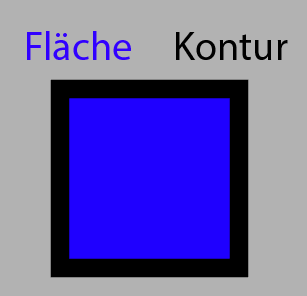
\includegraphics[width=0.4\textwidth]{design_abb4.png}
  \caption{Veranschaulichung von Fläche/Kontur}
\end{figure}

\leavevmode \\
\leavevmode \\
Also kann jedes Objekt mit einer Fläche und Kontur versehen werden. Es ist aber natürlich auch möglich nur eines der beiden, oder gar nichts auszuwählen, wobei letzteres in kaum einem Fall Sinn macht, da das Objekt dann komplett unsichtbar wäre. Zur einfachen Bedienung gibt es zwei Schaltflächen im Illustrator. Ein ausgefülltes Quadrat und die ausgefüllte Kontur eines Quadrats. Ein Doppelklick auf eines der beiden Elemente öffnet ein neues Fenster mit einem Farbwähler. Hier kann man mit Hilfe eines Schiebereglers und einer Art Koordinatensystem gewünschte Farben aussuchen. Genauer und somit auch zielführender, kann man die Farbwerte nach dem RGB-Modell, dem HSB-Modell, dem CMYK-Modell und hexadezimal angeben.\cite{farbselect}
\leavevmode \\
\leavevmode \\
RGB:
\leavevmode \\
Bei dem RGB-Modell setzen sich die Farben aus den drei Grundfarben Rot, Grün und Blau zusammen. Daher auch der Name. Die einzelnen Anteile sind von Null bis zu einem Wert von 255 definierbar. Mit Null mitgezählt macht das also 256 verschiedene Stufen, also entspricht das acht Bit pro Grundfarbe. Die Reihenfolge bei RGB ist wichtig. So steht der erste Wert für Rot, der zweite für Grün und der letzte für Blau. Zum Beispiel hat man mit den Werten 255/0/0 ein reines Rot mit einem Rotanteil von 100\%.\cite{rgb}
\leavevmode \\
\leavevmode \\
HSB:
\leavevmode \\
Dieses Farbraumsystem beschreibt Farben nicht durch Mischungen von Grundfarben, sondern durch die Eigenschaften der Farben. H steht für das englische Wort „hue“ und gibt den Farbton als Farbwinkel an. Also kann der Farbton von Null bis 360 Grad angegeben werden. S steht für „saturation“, also die Sättigung der Farbe. Diese beschreibt den Grauanteil der Farbe. Das heißt, dass ein Wert von null Prozent ein Grau ergeben würde und ein Wert von 100 Prozent einen voll gesättigten Farbton. B wird auch in Prozent angegeben und steht für „brightness“, also Helligkeit.\cite{hsb}\cite{hsbzwei}
\leavevmode \\
\leavevmode \\
CMYK:
\leavevmode \\
Hier stehen die Buchstaben für Cyan, Magenta, Yellow und Key. Cyan ist ein helles Blau mit grünlichem Ton. Bei Magenta handelt es sich um ein leicht violett getöntes Rot. Yellow ist ein helles strahlendes Gelb. Key ist einfach schwarz. Die Mischung aus Cyan, Magenta und Yellow würde zwar auch Schwarz ergeben, jedoch ist Key ein weiterer Parameter von CMYK, da das Schwarz aus den drei anderen Farben nicht besonders intensiv oder rein ist. Die Farbanteile der einzelnen Farben werden in Prozent angegeben. CMYK hat im Vergleich zu RGB einen sehr kleinen Farbraum. Somit kann man nicht das selbe Farbspektrum veranschaulichen. Es ist aber gut geeignet, um Objekte zu designen, die im Anschluss gedruckt werden sollen, da Drucker nicht das komplette RGB-Spektrum abdecken können. Je nachdem ob man mit RGB oder CMYK arbeitet, ist es empfehlenswert, den Dokumentfarbmodus im Illustrator entsprechen anzupassen.\cite{cmyk}
\leavevmode \\
\leavevmode \\
Hexadezimal:
\leavevmode \\
Hexadezimal ist im Prinzip eine andere Schreibweise für die RGB-Werte. Der Code besteht aus einem \# und daraufhin folgend sechs Zeichen. Diese können Null bis Neun und A bis F sein. Die ersten zwei Zeichen stehen für Rot, die zweiten für Grün und die dritten für Blau. Das bedeutet 256 verschiedene Möglichkeiten und acht Bit pro Farbe, also genau dieselben Werte, wie sie schon bei RGB zu lesen sind.\cite{hex}
\leavevmode \\
\leavevmode \\
Websichere Farben:
\leavevmode \\
In dem Farbwahlfenster gibt es außerdem die Möglichkeit, nur websichere Farben auswählbar zu machen. Das kann sehr hilfreich sein, da nicht jeder Browser alle Farben unterstützt. Wenn man websichere Farben nutzt, kann man sich als Designer sicher sein, dass jeder Nutzer genau die selben Farben sieht. Eine websichere Farbe hat im Hexadezimalcode an jeweils der Rot-, Grün- und Blaustelle die Zeichenkombinationen 00, 33, 66, 99, CC oder FF stehen. Das heißt aber, dass es nur 216 verschiedene Farben gibt, die als websicher gelten.\cite{websicher}
\leavevmode \\
\leavevmode \\
Wenn man nun eine Farbe für jeweils Fläche und Kontur festgelegt hat, kann man diese mit der Schaltfläche „Fläche und Kontur vertauschen“ einfach austauschen.
\leavevmode \\
\leavevmode \\
Füllarten:
\leavevmode \\
Unter der Fläche- und Konturschaltfläche befinden sich drei weitere kleinere Schaltflächen. Die Erste, ist die bisher beschriebene „Farbe“. Wenn man sie auswählt, wird die derzeitig ausgewählte Farbe auf die Fläche oder Kontur angewandt. Bei dem Logo wurde Farbe bei den Flächen, den schwarzen Linien, der Pupille, der Reflexion und der Kontur der Iris verwendet.\cite{flakonfarbe}
\leavevmode \\
Die zweite Schaltfläche ist der „Verlauf“. Mit ihr kann man Farbverläufe auf Flächen und Konturen anwenden. Es bieten sich neben den bereits erläuterten Farbwahloptionen auch die Möglichkeiten zu entscheiden, welche und wie viele Farben der Verlauf in welcher Reihenfolge abdecken soll, ob der Verlauf linear oder kreisförmig sein soll und welchen Winkel der Verlauf haben soll. Außerdem gibt es drei verschiedene Einstellungsmöglichkeiten, wie der Verlauf auf Konturen angewendet werden soll. Die Fläche, der Iris wurde mit einem Verlauf versehen. Dieser verläuft gleichmäßig und linear von Orange zu Grün, wobei Orange linksseitig und Grün rechtsseitig ist.\cite{verlauf}
\leavevmode \\
Bei der dritten Schaltfläche, „Ohne“, handelt es sich um die einfache Option, die Fläche oder Kontur leer zu lassen. Das bedeutet, wenn man beispielsweise bei einem Objekt eine schwarze Kontur ohne Fläche hat, ist die Fläche innerhalb der Kontur transparent und weiter hinten liegende Objekte sind dadurch sichtbar. Bei dem Logo wurde jedoch kein „Ohne“ verwendet.\cite{ohne}

\paragraph{Textwerkzeug}
\leavevmode \\
Zuletzt wurde bei dem Logo noch der Schriftzug „Insight“ angefügt. Dafür muss man einfach nur das Text-Werkzeug auswählen und damit an die Stelle klicken, an der der Text beginnen soll. Dieser kann dann einfach geschrieben werden. In den Texteinstellungen kann man noch Eigenschaften, wie Textgröße, Font und Zeilenabstand angeben\cite{fonts}
Für den Schriftzug des Logos wurde Parisien Night Oblique als Font gewählt. Diese Schrift wurde wegen des Logos in das Corporate Design aufgenommen. Die schwungvolle dynamische Linienführung soll an die Eigenschaften, des Logos erinnern. Zusammen ergeben Signet und Schriftzug ein stimmiges Bild, was zeigt, dass die Wahl der richtigen Font für ein Logo ein essenzieller Faktor ist. Näheres zur Typografie, ist beim Corporate Design zu lesen.\cite{textwerkzeug}
\leavevmode \\
\leavevmode \\
Verformen mit Hüllen:
\leavevmode \\
Die Schrift sollte sich an das Logo schmiegen, welches eine sehr runde Erscheinungsform hat. Deshalb musste die Schrift gekrümmt und rotiert werden. Bei der Rotation handelte es sich um eine einfache Transformation des Objekts, welche mit dem Cursor, oder manuell mit der Angabe von Winkelgrad umgesetzt werden konnte. Um die Schrift jedoch entlang der Linien zu krümmen, wurden Hüllen verwendet. Bei Hüllen handelt es sich um Objekte, die verwendet werden, um ausgewählte Objekte zu verformen. Dafür findet man unter der Schaltfläche „Objekt“ die Kategorie „Verzerrungshülle“. Die erste Option, „Mit Verkrümmung erstellen…“, ist gleich die, die benötigt wurde. Es öffnet sich ein neues Fenster, in welchem man die Art der Verkrümmung angeben kann. Im Fall des Schriftzuges ist diese Art „Bogen“. Um nun den Anfang und das Ende des Textes nach oben zu biegen, um ihn an das Logo anzupassen, muss nur noch ein negativer Prozentwert angegeben werden. Minus 20 Prozent erwiesen sich als eine sehr leichte, aber doch passende Krümmung.\cite{huellen}
\leavevmode \\
\leavevmode \\
SVG:
\leavevmode \\
Nachdem es fertiggestellt wurde, wurde das Logo, so wie fast alle anderen im Illustrator erstellten Grafiken, als SVG abgespeichert. Hierbei handelt es sich um ein auf XML basierendes Dateiformat, welches genutzt wird um Vektorgrafiken im Web darzustellen.\cite{svg}

\begin{figure}[H] 
  \centering
     
\includegraphics[width=0.4\textwidth]{design_abb5.png}
  \caption{Logo Endergebnis}
\end{figure}

\subsection{Visitenkarten}
\subsubsection{Zweck}
Die Visitenkarten von Insight wurden für den Tag der offenen Tür und den Innovation Day an der HTL Rennweg gedruckt. Ihr Zweck war es, Besucher, der Schule und Unternehmen auf das Projekt aufmerksam zu machen und ihnen die Möglichkeit zu geben, später Informationen zu dem Projekt zu finden, oder Kontakt zu dem Team aufzunehmen.
\subsubsection{Umsetzung}

\paragraph{Neue Datei}
\leavevmode \\
Auch die Visitenkarte wurde im Adobe Illustrator entworfen. Das erste worauf geachtet werden musste ist, dass die Datei die richtige Größe hat. Die ausgewählte Druckerei verlangte für jeweils die Vorder- und Rückseite, der Visitenkarte ein JPG, welches 85 Millimeter breit ist und 55 Millimeter hoch. Der Illustrator bietet bei der Erstellung der Datei die Option, Höhe und Breite in Millimetern anzugeben, was dem Entwurf der Karte sehr zu Gute kam. Der eingestellte Farbraum in den Dokumenteinstellungen war in diesem Fall CMYK, da dies für den anschließenden Druck optimal war. Außerdem wurde es von der Druckerei empfohlen, diesen Farbraum zu nutzen.\cite{newdoc}

\paragraph{Vorderseite}
\leavevmode \\
Auf der Vorderseite sollten alle wichtigen Informationen stehen, welche geplant waren auf der Visitenkarte preis zu geben. Dazu gehört das Logo, die URL der Website, die Mailadresse, des Teams und der Name der Schule.
\leavevmode \\
Der Name des Projekts konnte vernachlässigt werden, da er sich bereits im Logo befindet. So wurde überflüssiger Content vermieden und das Gesamtbild aufgeräumter gehalten. Das Layout ist zentriert und die Elemente untereinander angeordnet. Das Schmalste ganz oben und das Breiteste unten. So erscheint der Content der Vorderseite wie ein Dreieck oder Pyramide, also ein Objekt womit der Betrachter vertraut ist. In einem, nach Corporate Design, orangenen Footer, ist optisch abgegrenzt von den restlichen Inhalten, der Name der Schule.
\leavevmode \\
\leavevmode \\
Intelligente Hilfslinien: 
\leavevmode \\
Zur Positionierung der Elemente auf der Karte, wurden intelligente Hilfslinien verwendet. Diese lassen Ankerpunkte von Objekten, anhand von Ankerpunkten anderer Objekte relativ positionieren. Das heißt, wenn diese Hilfslinien aktiviert sind, lassen sich Objekte so positionieren, dass sie zum Beispiel mittig von einem anderen Objekt liegen, oder an einer markanten Stelle vertikal oder horizontal gleich mit einer markanten Stelle des Anderen Objektes liegen. So wurden alle Elemente perfekt mittig untereinander platziert. Die selbe Technik wurde beim Logo verwendet, um die Pupille in der Mitte der Iris zu platzieren. Für die Schrift wurde das Textwerkzeug verwendet. Um das Logo auf die Karte zu übertragen, wurden die Pfade kopiert und eingefügt. Beim Verkleinern auf eine angemessene Größe, fiel die statische Stärke der Kontur der Iris auf. Diese musste manuell verringert werden, damit das Gesamtbild dem Original entspricht.\cite{lines}

\begin{figure}[H] 
  \centering
     
\includegraphics[width=0.5\textwidth]{design_abb6.png}
  \caption{Vorderseite der Visitenkarte}
\end{figure}

\paragraph{Rückseite}
\leavevmode \\
Auf der Rückseite der Visitenkarte prangt eine großer, mit Hilfslinien zentrierter, orange-grüner QR-Code, der den Scannenden auf die Website von Insight bringt. Der Code wurde per Eingabe der URL in einem Online-Tool generiert und gedownloadet.\cite{qrc} Das erhaltene PNG wurde dann im Photoshop mit den Farben des Corporate Designs eingefärbt.
\leavevmode \\
\leavevmode \\
QR-Code:  
\leavevmode \\
QR steht für „Quick Response“. Bei dem Code handelt es sich um eine quadratische Matrix aus kleineren weißen und schwarzen Quadraten. Die Codes können mit Hilfe einer App von Handykameras gelesen werden und so Informationen oder Daten ausgeben. Im Fall der Visitenkarte, handelt es sich um eine URL. Damit der Code funktioniert, egal wie er gedreht ist, befinden sich in drei von vier Ecken der Matrix größere Quadrate. An ihnen wird sich am Scanvorgang orientiert, wie herum der Code korrekt zu lesen ist.\cite{qrnutzen}

\begin{figure}[H] 
  \centering
     
\includegraphics[width=0.5\textwidth]{design_abb7.png}
  \caption{Rückseite der Visitenkarte}
\end{figure}

\subsection{Designelemente}
\subsubsection{Zweck}
Mit Designelementen sind weitere selbst erstellte Grafiken gemeint, die auf der Webseite Verwendung gefunden haben. Manche dieser Grafiken wurden auf Grund von Änderungen nicht in die finale Version der Website aufgenommen. Die folgenden Grafiken sind Teil, der finalen Version und als userinteraktives Element implementiert.
\leavevmode \\
\leavevmode \\
Schrödingers Katze:
\leavevmode \\
Die Katze in der Box wurde wie das Logo zuerst im Photoshop skizziert und dann im Illustrator mit dem Zeichenstift-Werkzeug nachgezeichnet. Im Gegensatz zu den bisher erwähnten Grafiken, wurden die Kopier- und Einfügeoption viel öfter verwendet. Um Objekte zu kopieren, muss man sie einfach nur auswählen und die Tastenkombination „Strg“ + „C“ verwenden. Um ein Objekt einzufügen nutzt man „Strg“ + „V“. Die Funktion wurde bei der geschlossenen Box für die Schrauben und diverse Planken genutzt, damit sie exakt dieselbe Größe haben. Bei der offenen Box wurde Kopieren und Einfügen wiederum für das Holz benutzt, aber diesmal auch für die Maserung, die Augen und Pfoten der Katze und sogar ihren Mund. Verwendet wurde die Katze im Chapter 7 der Website. Das Spiel heißt Schrödingers Katze.\cite{cap}

\begin{figure}[H] 
  \centering
     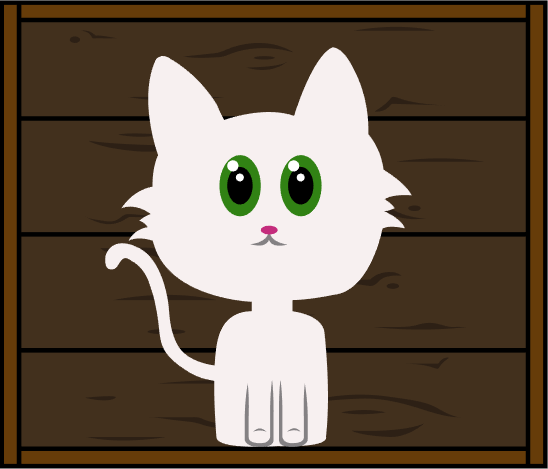
\includegraphics[width=0.4\textwidth]{design_abb8.png}
  \caption{Katze Endergebnis}
\end{figure}

\leavevmode \\
\leavevmode \\
Rakete: 
\leavevmode \\
Auch die Rakete wurde mit dem Zeichenstift-Werkzeug erstellt. Jedoch nur eine Hälfte. Um die Rakete symmetrisch zu machen, wurde nur die Hälfte gezeichnet, dann durch Kopieren und Einfügen dupliziert und anschließend wurde die kopierte Hälfte gespiegelt und an die zweite Hälfte angefügt. Gespiegelt wurde das Objekt mit dem Spiegeln-Werkzeug. Mit Hilfe der Shift-Taste konnte man den Spiegel-Winkel auf 45-Grad-Schritte beschränken, was ein gespiegeltes Gegenstück erzeugte, welches perfekt an sein Ursprungsobjekt anschloss. Die Rakete war ursprünglich als Button auf der Website geplant, hat aber nun als userinteraktives Element bei „Verschiebe das Universum“ seinen Platz gefunden.\cite{spiegel}

\begin{figure}[H] 
  \centering
     
\includegraphics[width=0.4\textwidth]{design_abb9.png}
  \caption{Rakete Endergebnis}
\end{figure}

\leavevmode \\
\leavevmode \\
Bezirkkarte von Wien:
\leavevmode \\
Es war ursprünglich geplant ein userinteraktives Element auf der Website einzubauen, welches eine Karte von Wien darstellen sollte. Je nachdem über welchem Bezirk man sich mit dem Cursor befand, sollte dieser eingefärbt werden. Dafür wurde eine farblose Karte benötigt und und jeweils eine Karte, wo jeweils ein Bezirk eingefärbt war. Die Karte war eine nervenzerreißende, lange Arbeit, da zu dem Zeitpunkt noch nicht an den Pathfinder gedacht wurde. Das heißt anstatt jeden Bezirk in ein eigenes, einfärbbares Objekt zu verwandeln, wurde für jeden Bezirk ein extra Objekt gezeichnet, welches eingefärbt werden konnte. Danach wurde für die leere Karte ein SVG abgespeichert und für jeden Bezirk zwei, da noch nicht feststand, ob die Bezirke Grün oder Orange sein sollten. Das Umfärben, Auswählen und und einzelne Abspeichern hat sehr viel Arbeitszeit in Anspruch genommen.

\begin{figure}[H] 
  \centering
     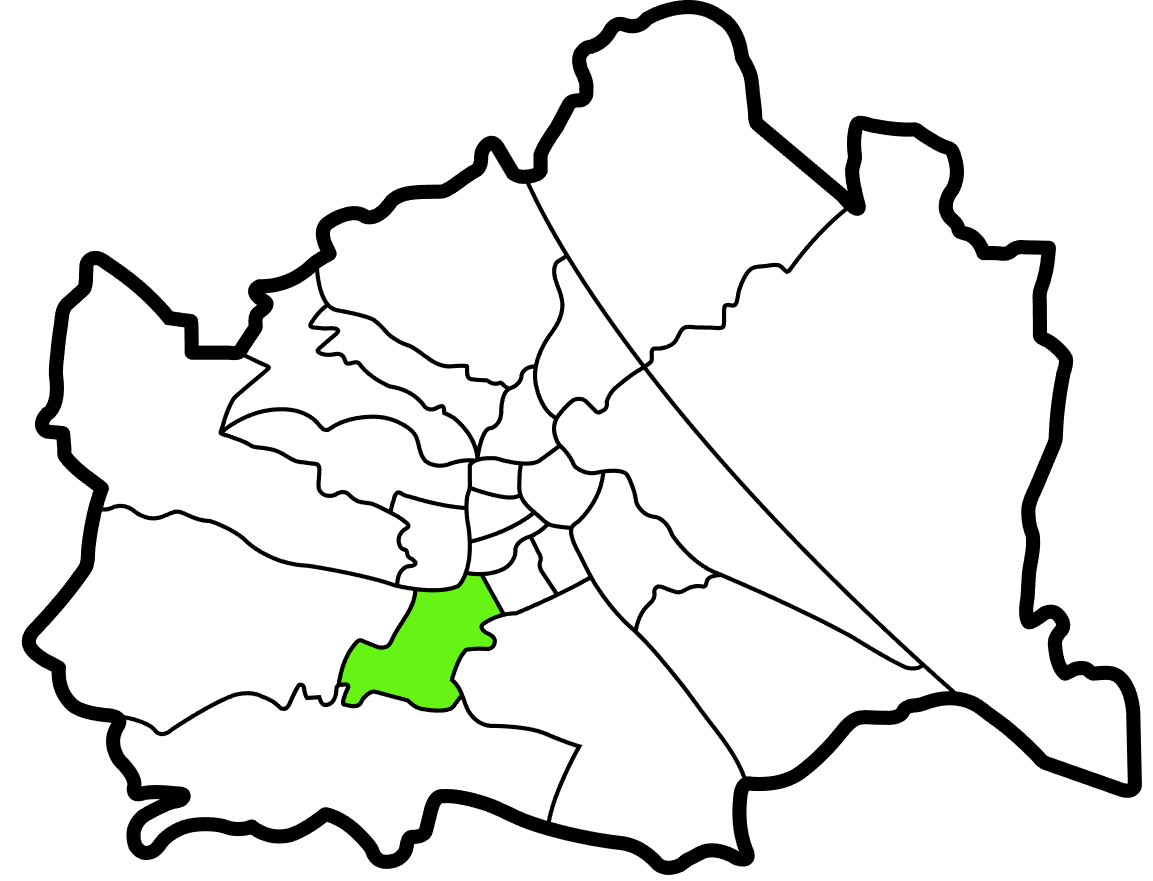
\includegraphics[width=0.4\textwidth]{design_abb10.png}
  \caption{Wienkarte Endergebnis}
\end{figure}

\chapter{Webauftritt}

\renewcommand{\kapitelautor}{Autor: Hatice Akyokus}

In diesem Kapitel wird der Webauftritt erläutert. Der Webauftritt ist der wichtigste Bestandteil der Diplomarbeit, da sich alle Elemente auf dieser befinden.
 
\section{Intention}
Um die Zielgruppe am Besten zu erreichen, wurde eine Webseite erstellt. In dem Zeitalter des Internets ist es sehr wichtig, den Webauftritt auf eine kreative Art und Weise zu gestalten. Vor allem, da diese Diplomarbeiten Informationen über die Medientechnik vermitteln möchte. Eine Informationsseite, welche aufzählt, was an der HTL Rennweg beigebracht wird, wäre langweilig und würde die Zielgruppe nicht erreichen. Aus diesem Grund wurden viele Brainstormings durchgeführt, um die beste Vorangehensweise zu ermitteln. Die große Schwierigkeit hierbei war es, die Webseite an die Zielgruppe anzupassen, da sie die Medientechnik nicht kennen. Daher mussten alle Erklärungen und technische Aspekte, so einfach wie möglich erklärt werden, um sie nicht zu verschrecken. Durch die Problematik am Tag der offenen Tür, soll die Webseite auch Missverständnisse beseitigen und dafür sorgen, dass User eine Entscheidung treffen können, die sie später nicht bereuen. 

\section{Inhalt}
Die Entscheidung, welche Inhalte auf der Webseite zu sehen sind, war nicht leicht, da die Medientechnik ein sehr großer Bereich ist. Sehr früh hat sich das Team darauf geeinigt, die Medientechnik mit der Größe des Universums zu vergleichen und die Webseite in einem „Space-Theme“ zu halten. Wie bei jedem Webauftritt üblich, enthält diese eine Startseite, welche einen Vorgeschmack geben soll und weitere Informationen bietet. Informationen über die Medientechnik finden sich in zehn Lektionen, welche das Team aufbereitet hat und zeigt, was in den fünf Jahren Medientechnik beigebracht wird. Da sich der Lehrplan allerdings ändern wird, wurden die Lektionen allgemein gehalten und bieten einen Einblick in die Basics der Mediengestaltung, Animationen und Spiele. Um die Informationen spannender zu präsentieren, wurden interaktive Elemente hinzugefügt, welche die User für die Medientechnik begeistern sollen. Da Videos auch eine wichtige Rolle in der Medientechnik spielen, wurden Interviews und auch ein Animationsvideo gedreht, welche es als Ziel hatten, die User über die Schule im Allgemeinen und die Medientechnik zu informieren. Durch diese ganzen Elemente soll gewährleistet werden, dass die User über die HTL Rennweg informiert sind und eine Entscheidung treffen können. 

\section{Hosting}
Webhosting stellt Speicherplatz in Internet bereit. Für dies ist ein leistungsstarker Rechner notwendig. Um die Inhalte jederzeit abrufen zu können, ist deshalb eine Internetverbindung notwendig. Je nach Anbieter und Angebot, ändert sich der Leistungsumfang im Webhosting. \cite{webhosting} Das Team entschied sich anfangs für das Webhosting durch easyname.at, weil es ein Jahr lang kostenlos ist und viel Speicherplatz zur Verfügung stellt. Allerdings hat sich nach kurzer Zeit herausgestellt, dass die Leistung nicht den Wünschen des Teams entsprach und somit musste die Domain, welche im Angebot enthalten war, transferiert werden. Nach einer langen Suche, nach einem geeigneten Webhoster, stieß das Diplomarbeitsteam auf syhost.at, was auch ein Angebot bietet, welches ein Jahr lang kostenfrei ist. Einzig die Kosten für die Domaintransferierung mussten bezahlt werden. Die Leistung von syhost.at entsprach mehr den Vorstellungen des Teams. Mittels dem File Transfer Protocol Client „Filezilla“, werden die Webseiten hochgeladen und den Usern zur Verfügung gestellt. 


\section{Bildquellen}
Alle verwendeten Bilder wurden von der Webseite unsplash.com heruntergeladen. Unsplash.com ist eine Webseite, auf der User Bilder, die sie selbst geschossen haben, hochladen können. Diese können von anderen Usern kostenlos heruntergeladen werden. Weiters wurden kostenlose Vektorgrafiken von der Webseite flaticon.com verwendet. Dies ist eine Webseite, welches Vektorgrafiken in verschiedenen Formaten anbietet. Es gibt kostenpflichtige und kostenfreie Grafiken, die frei anpassbar sind. Für die Webseite wurden kostenfreie Vektorgrafiken verwendet. Im Rahmen der Diplomarbeit wurden Bilder verwendet, die dem Corporate Design entsprechen und zu dem Thema der Diplomarbeit passen. Das Team entschied sich für ein „Space-Theme“, welches die Größe der Medientechnik grafisch darstellen sollte. 

\section{Frameworks und Libraries} 
Framework heißt übersetzt Rahmenkonstruktion und wird häufig bei Webseiten verwendet. Sie dienen als Gerüst zum Programmieren und erleichtern die Arbeit, die damit verbunden ist. Dabei ist das Framework selbst kein Programm, sondern ein Rahmen, welcher den Inhalt ansprechend präsentiert. \cite{framework}

\subsection{Content Delivery Network}
Ein Content Delivery Network sorgt für eine schnelle und zuverlässige Auslieferung von Medieninhalten, welche mit Hilfe von Caching im Internet vorgehalten werden. \cite{cdn}

\begin{quote}
"Das CDN besteht aus einem Ursprungsserver (Originserver), auf dem die zu verteilenden Inhalte ablegt [sic!] werden, vielen Replica-Servern, welche die Kopien der Inhalte vorhalten, sowie einem Distributionssystem, das die Inhalte auf den Replica-Servern verteilt. Für die Umleitung der Nutzeranfragen auf die einzelnen Replica-Server sorgt ein Request-Routing-System. Nachdem ein Client eine Anfrage an das Content Delivery Network gesendet hat, wählt das Request-Routing-System den geeigneten Replica-Server aus. Bei der Auswahl bezieht es Kennzahlen über deren aktuelle Belastung (CPU-Auslastung, Menge der aktiven Verbindungen etc.) und über die Netzwerkverbindung zwischen dem anfragenden System und dem Server mit ein. Ist der Server ausgewählt, wird die Nutzeranfrageentsprechend umgeleitet." \cite{zitatcdn}
\end{quote}
Die Vorteile eines Content Delivery Networks sind die schnellen Ladezeiten, die hohe Ausfallsicherheit und eine optimale globale Lastverteilung. Allerdings kann man die Dokumente, welche man von einem Content Delivery Network bezieht, nicht optimieren. Vor allem bei CSS-Frameworks ist dies ein großer Nachteil, weil man die CSS-Styles überschreiben muss. Außerdem gibt es keine Garantie, dass die Webseite pre-cached wurde, da vor allem mobile Geräte einen kleinen und ineffizienten Cache haben. Ein wichtiger Punkt ist, dass Content Delivery Networks nicht in allen Ländern zur Verfügung stehen, da sie aus geografischen oder politischen Gründen blockiert werden. Allerdings ist dies kein Problem für die Diplomarbeit Insight, weil die Webseite nur für User in Österreich gedacht ist. \cite{cdnnachteile}
\leavevmode \\
Da FontAwesome verwendet wurde, welche eine große Datei zum Herunterladen ist, entschied sich das Team dazu ein Content Delivery Network zu verwenden. Das CSS-Framework Foundation und alle anderen JavaScript-Frameworks wurden heruntergeladen und deren CSS beziehungsweise JavaScript Dokumente eingebunden. Dies hat den Vorteil, dass man die CSS und JavaScript Dokumente nach Belieben optimieren kann. Somit hat man mehr Kontrolle über das Framework. Weiters spielt die Internetgeschwindigkeit eine große Rolle. Die Webseite wird, wenn das Framework lokal gespeichert ist, bei einem schlechten Internetzugang schneller geladen.
\subsection{CSS-Frameworks} 
Ein CSS-Framework sorgt für das Layout der Webseite. Da sie die meiste Programmierarbeit abnimmt, kann man produktiver arbeiten und Fehler vermeiden. Weiters, hat man einen besseren Workflow im Team und eine optimale Browser-Kompatibilität. 
Ein solches Framework beinhaltet vordefinierte CSS-Klassen, welche einfach zu benutzen sind, typographische Style Definitionen und ein Grid System.  
Allerdings braucht man mehr Zeit, um das Framework zu verstehen. Deswegen ist es sehr wichtig, dass das Framework eine sehr gute Dokumentation hat, welche gut gepflegt wird. Größere CSS-Frameworks bieten auch JavaScript-Files, welche erweiterte Funktionen bieten. Im Rahmen der Diplomarbeit wurde das CSS-Framework Foundation verwendet.\cite{cssframework}
\subsubsection{Bootstrap oder Foundation}
Das CSS-Framework Foundation hat eine kleine Community und somit sind die Foren eher leer und bieten nicht mehrere Antworten auf eine Frage. Die Dokumentation ist zwar gut, aber manche Fehler konnten auch mit dieser nicht gelöst werden. Deswegen überlegte sich das Team, in dem Anfangsstadium der Diplomarbeit, auf das CSS-Framework Bootstrap umzusteigen. Um eine geeignete Entscheidung treffen zu können, wurden beide Frameworks verglichen. Bootstrap ist um einiges beliebter als Foundation und hat eine größere Community. Genauso wie Foundation basiert Bootstrap auch auf einem Grid-System. Während Bootstrap auf einem Flex-Grid basiert, bietet Foundation mehrere Möglichkeiten an Grids an. Es gibt ein XY Grid, welches horizontal oder vertikal angelegt werden kann. Außerdem kann man der Grid noch weitere Eigenschaften zuweisen. \cite{bootstrapfoundation} Weiters hat Foundation eine Topbar, welche eine Navigationsleiste ist, welche sich mehr auf die Struktur konzentriert als auf das Design, was bedeutet, dass man die Navigationsleiste individuell designen muss. Dies ist ein Vor- und Nachteil, da die Navigationsleiste individuell gestaltbar ist und nicht zwingend wie andere Navigationsleisten aussieht, aber dahinter steckt wiederrum Programmierarbeit, was bei Bootstrap nicht der Fall ist. Doch die Navigationen von Webseiten, die mit dem Framework Bootstrap entwickelt wurden, haben ein für Bootstrap typisches Styling. \cite{bootstrapfoundation2} Allerdings hat Bootstrap in Sachen wie den Support für mobile Geräte die Nase vorne. Weiters bietet Bootstrap sehr viele Templates, welche sehr beliebt sind. Bootstrap konzentriert sich, wie bereits erwähnt, mehr auf das Design und Foundation hingegen legt sehr viel Wert auf Responsiveness und Funktionalitäten. Für Anfänger wird Bootstrap empfohlen. Das Team entschied sich im Endeffekt für Foundation, da es eine neue Herausforderung für das Team ist und Foundation einen fluiden Ansatz bietet und mehrere Funktionen bietet als Bootstrap. \cite{bootstrapfoundation3}
\paragraph{Foundation} \leavevmode \\
Foundation ist ein CSS-Framework und wirbt damit, für jedes Gerät geeignet zu sein. Es sorgt für Responsiveness und Einfachheit beim Designen der Webseite. Foundation basiert auf dem Mobile First Prinzip, was bedeutet, dass die Darstellung auf mobilen Endgeräten die höchste Priorität hat. \cite{mobilefirst} Außerdem bietet das Framework die Möglichkeit, alle Elemente nach Belieben zu ändern. Mit ihren vordefinierten Klassen sorgt das Framework für einen sauberen und effizienten Code, welcher im optimalsten Fall leicht zu verstehen ist. Die einzige Herausforderung war es, sich in das Framework einzuarbeiten, welches etwas Zeit beanspruchte. \cite{foundationwebsite}
\paragraph{Slick Slider} \leavevmode \\
Slick Slider ist ein Framework, welches hauptsächlich für Slider gedacht ist. Da die Webseite dieser Diplomarbeit auf diesem Prinzip beruht, entschied sich das Team dazu, Slick Slider zu verwenden. Der Entwickler dieses Frameworks wirbt für Slick mit folgendem Slogan: „Slick – the last carousel you’ll ever need“ \cite{slick}. Slick ist sehr einfach zu bedienen, da die Programmierarbeit sehr minimal ist. Die nötigen Methoden werden bereits vom Framework angeboten, wobei man sehr viel anpassen kann. Somit muss man die vordefinierten Klassen nicht verwenden und kann es vom Aufbau her, so gestalten wie man möchte. Dies wurde in der Diplomarbeit natürlich ausgenutzt, um die Webseite einzigartig erscheinen zu lassen. Slick bietet dem Nutzer sehr viele Möglichkeiten an, die Slider zu steuern oder zu gestalten und ist responsive und basiert ebenfalls auf dem mobile-first Prinzip. Außerdem bietet Slick den Nutzern die Möglichkeit Breakpoints zu setzen.

\lstset{
  frame=leftline,
  xleftmargin=.05\textwidth
}
\begin{lstlisting}

$(document).on('ready', function() {
	$('.content').slick({
		infinite: false,
		speed: 500,
		fade: true,
		cssEase: 'linear'
	});
});
\end{lstlisting} \leavevmode \newline
Der Parameter infinite sagt aus, ob man, nachdem man an das letzte Slide angekommen ist, wieder an das erste Slide gelangt oder nicht mehr weiterschalten kann. Aus Storyzwecken entschied sich das Team dazu, dies auf den Wert "false" zu setzen. Um keinen typischen Slider Effekt zu erzielen, wurde der Parameter fade auf "true" gesetzt.

\lstset{
  frame=leftline,
  xleftmargin=.05\textwidth
}
\begin{lstlisting}

$('.next').click(function(){
	$('.content').slick('slickNext');
});

$('.previous').click(function(){
	$('.content').slick('slickPrev');
});
\end{lstlisting} \leavevmode \newline
Das Team hat außerdem eigene Buttons zum Weiterschalten definiert, welche sich nicht, wie bei Slidern üblich, links und rechts, sondern unterhalb befinden. Slick wurde ebenfalls heruntergeladen und lokal hinzugefügt.
\paragraph{Create JS} \leavevmode \\
Create JS ist eine Sammlung von Libraries, welche entweder zusammen arbeiten oder individuell angewendet werden können. Diese Libraries basieren auf JavaScript und bestehen aus:
\begin{itemize}
\item EaselJS
\item TweenJS
\item SoundJS
\item PreloadJS
\end{itemize}
EaselJS wurde für diese Diplomarbeit verwendet und ist dafür gedacht, dass man besser mit dem HTML 5 Canvas arbeiten kann und wurde für die siebte Lektion verwendet. \cite{createjs}
\paragraph{interact.js} \leavevmode \\
Interact.js ist ein JavaScript-Framework, welches für Drag and Drop und Muti-Touch-Gesten gedacht ist. In der Diplomarbeit wird sie für das sechste Kapitel verwendet. \cite{interact}
\section{Responsiveness}
Responsive Webdesign bedeutet, dass sich der Inhalt einer Webseite an die Bildschirmauflösung des Endgeräts anpasst. Der steigende Marktanteil von Smartphones und Tablets zwingt die Entwicklung von responsiven Webseiten. Dabei soll die Trennung zwischen einer Mobil- und Desktopversion vermieden werden, da dadurch ein erhöhter Pflegeaufwand entsteht. Durch die stetige Änderung von Tablet- und Smartphoneformate, werden mehrere Versionen von Nöten sein und das soll mit einer responsiven Webseite verhindert werden.
Um zu gewährleisten, dass die Webseite auf allen Endgeräten einwandfrei funktioniert, wurde auf eine responsive Webseite einen sehr großen Wert gelegt. Vor allem, da die Webseite sehr viele Bilder enthält.
\begin{quote}
"Responsive Webdesign ist kein Trend! Studien zum Absatz mobiler Endgeräte belegen eine stetige Zunahme der Verkäufe von Tablets und Smartphones. Diese Entwicklung wird nicht nur von der Fachszene mit Euphorie verfolgt, es gibt auch fast täglich neue Entwicklungen zum Thema der technischen und grafischen Umsetzung von Webseiten für mobile Endgeräte. Responsive Webdesign spielt mit der geräteübergreifenden Flexibilität eine tragende Rolle in dieser Bewegung die sich zunehmend zu einem Standard entwickelt." \cite{responsive}
\end{quote}
Durch ein responsives Design wird eine bessere Bedienbarkeit gewährleistet und somit die Bounce-Rate deutlich reduziert. Außerdem ergibt sich weniger Wartungsaufwand bei Updates.  Das CSS-Framework hilft dabei als Gerüst, die Webseite responsiv zu machen. Allerdings muss auch nachgeholfen werden und dies erfolgte hauptsächlich mit Flexbox. Dies ist eine sehr einfache Möglichkeit, flexible Layouts zu erstellen, ohne CSS-Einstellungen, wie position zu verwenden. In der Diplomarbeit wurde sie hauptsächlich dafür verwendet, Elemente zu zentrieren, denn dies erweist sich, vor allem für das vertikale Zentrieren von Elementen, als kompliziert. \cite{responsive}
\lstset{
  frame=leftline,
  xleftmargin=.05\textwidth
}
\begin{lstlisting}

.content{
	height: 100vh;
	width: 90%;
	position: relative;
	top: 10vh;
	margin-left: 5vw;
	margin-right: 5vw;
	display: flex;
	justify-content: center;
	align-items: center;
}

\end{lstlisting} \leavevmode \newline
Wie in den CSS Stylings zu erkennen ist, wird auf das Element mit der Klasse content, eine Flexbox angewendet. Alle Kindelemente von content werden, sowohl horizontal als auch vertikal zentriert, angezeigt. Außerdem wurden bei den Größenangaben keine Werte in Pixel angegeben. Das Pixel ist eine absolute CSS Einheit und darin liegt auch das Problem, denn sobald die Webseite verkleinert wird, bewegt sich der Inhalt nicht mit und ist somit nicht responsiv. Deswegen wurden relative CSS Einheiten, wie vw, vh und rem verwendet. Die Einheiten vw und vh stehen für viewport width und viewport height und entsprechen dem 100. Teil der Breite des Anzeigebereiches. Allerdings werden sie vom Internet Explorer erst ab Version 9 unterstützt. Die Einheiten viewport width und viewport height wurden für Div-Boxen verwendet, da es wichtig ist, dass sie responsiv sind.\cite{wiki}  Für Schriftarten wurden die Einheiten rem, root em und em verwendet. 
\begin{quote}
„rem verhält sich genauso wie em mit dem einzigen Unterschied, dass das sich der rem-Wert am Root-Element orientiert (also an der Schriftgröße, für body bzw. html), statt sich wie em an der Schriftgröße des jeweiligen Eltern-Elements zu orientieren.“ \cite{remzitat}
\end{quote}
Da rem nicht von älteren Browsern unterstützt wird, musste eine Fallback-Lösung in px im Stylesheet definiert werden. \cite{remzitat}  Außerdem wurden Breakpoints eingearbeitet, um eine Responsiveness, vor allem für mobile Geräte, zu gewährleisten. Ein Breakpoint wird durch eine Media Query definiert.
\subsection{Startseite}
Die Startseite ist eine wichtige Seite, welche das Interesse anregen soll. Es war dem Team sehr wichtig, die Startseite so modern wie möglich zu gestalten, um den User dazu zu bringen die Webseite zu erkunden. Auf der Navigationsleiste befindet sich das Logo und weitere Links, über uns, Download, Kontakt und ein FAQ. Diese sind sehr simpel gehalten. Die Navigationsleiste ist schlicht gehalten und weiß. Die Schrift ist in dem orange des Corporate Designs und wenn man mit der Maus über die Links fährt, werden sie grün. Die Navigation besteht aus drei Containern, wobei eines das Logo enthält, eines welches bei Verkleinern des Bildschirms ein Burger Menü erscheinen lässt und eines, welche die Links zu den erwähnten Links enthält. Ein Burger Menü, ist ein Icon, welches beim Klick eine versteckte Navigation erscheinen lässt. Das ist vor allem bei mobilen Geräten sehr nützlich.\cite{burgermenu} Die Klasse „linkactive“, hebt die Seite, auf der man sich gerade befindet, hervor.  \newpage

\lstset{
  frame=leftline,
  breaklines=true,
}
\begin{lstlisting}[language=HTML, basicstyle=\scriptsize]
<div class="fixed">
	<div class="top-bar" data-topbar role="navigation">
		<div class="logo-wrapper">
			<div class="logo">
				<a href="../index.html">
					<img class="logo_img" src="../images/logo.svg">
				</a>
			</div>
		</div>

		<div class="title-bar" data-responsive-toggle="resmenu" data-hide-for="medium">
			<div class="title-bar-right">
				<button class="menu-icon" type="button" data-toggle="resmenu"></button>
				<div class="title-bar-title">Men&uuml;</div>
			</div>
		</div>

		<div class="top-bar-right" data-magellan id="resmenu">
			<ul class="vertical medium-horizontal menu">
				<li><a href="../download.html">DOWNLOAD</a></li>
				<li><a href="../faq.html">FAQ</a></li>
				<li><a href="../kontakt.html">KONTAKT</a></li>
			</ul>
		</div>
	</div>
</div>
\end{lstlisting} \leavevmode \newline
Die Startseite wurde mit jQuery entwickelt. Mittels der Library, parallax.js, wurde ein Parallax Effekt implementiert. 
\begin{figure}[ht]
	\centering				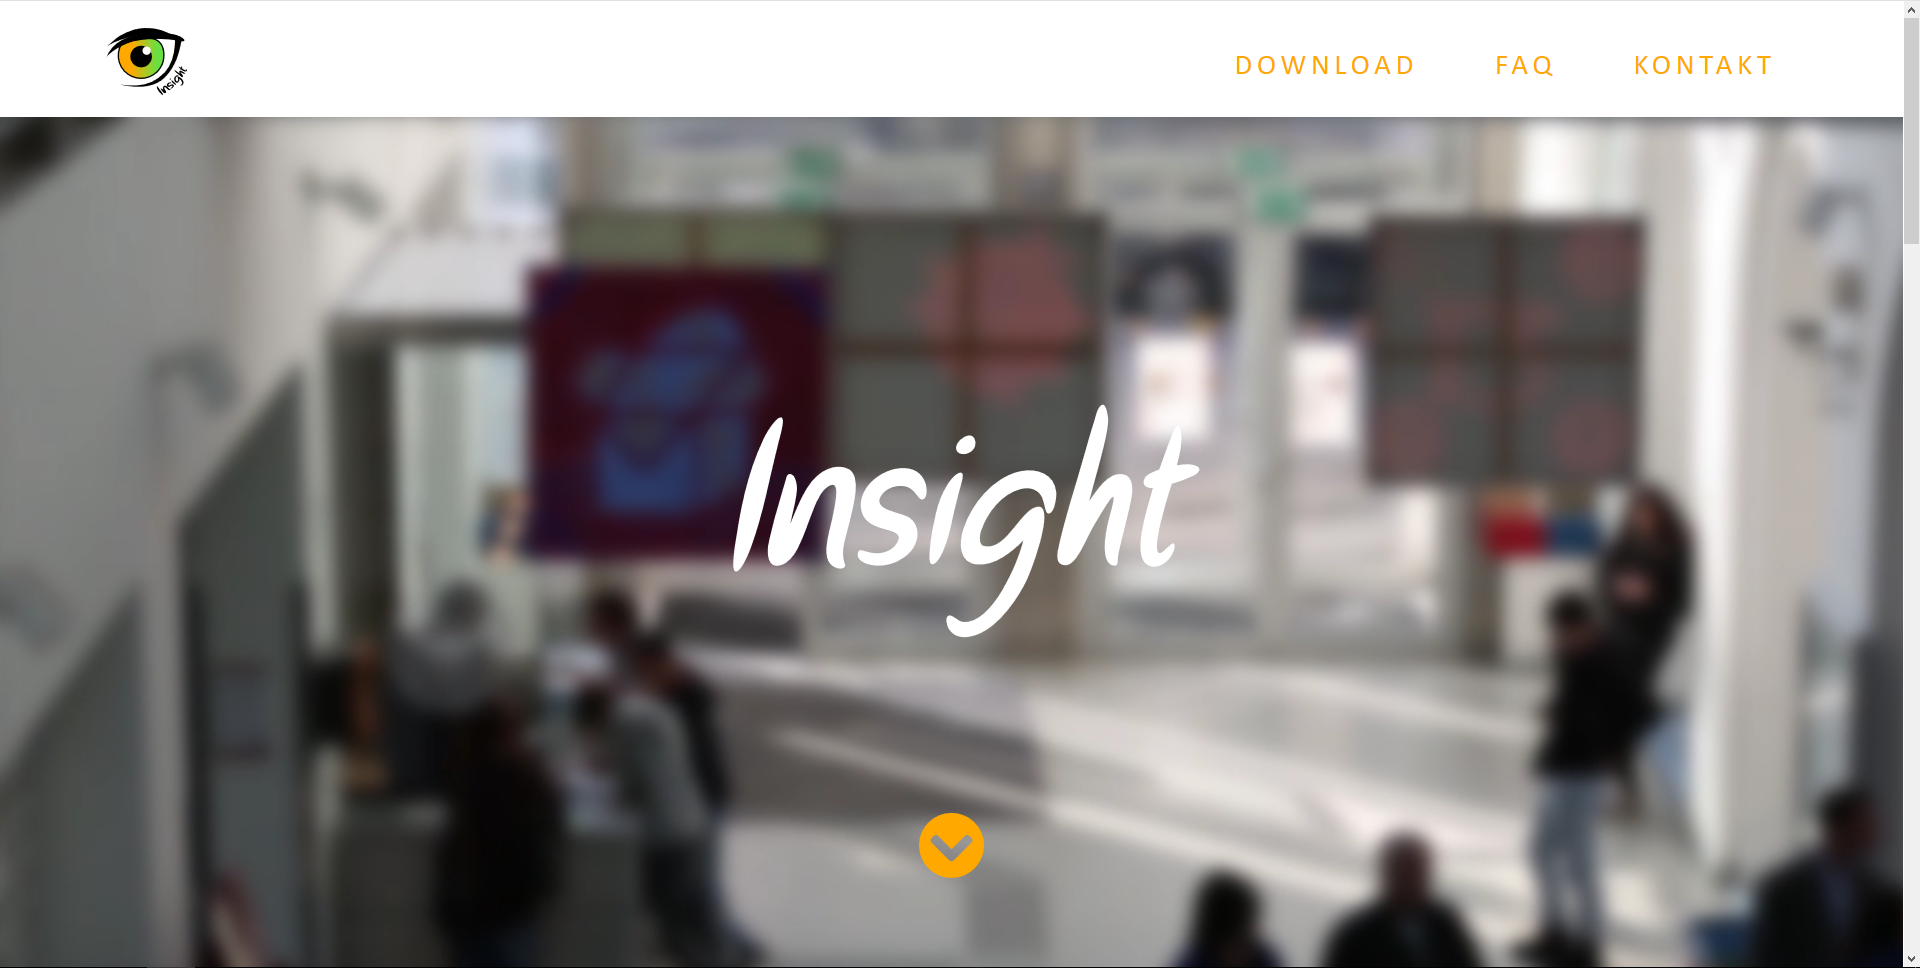
\includegraphics[width=12cm,height=12cm,keepaspectratio]{webseite_abb5} 
	\caption{Die Startseite}
\end{figure}
\begin{quote}
"Parallax Scrolling, oft auch Parallax Design, ist ein Begriff aus dem Bereich des Webdesigns. Es handelt sich letztendlich um einen Designansatz, der erzeugt wird, indem unterschiedliche Ebenen erstellt und asynchron gegeneinander geschoben werden - wie auf dieser Seite oft zu beobachten ist." \cite{parallaxzitat}
\end{quote}
Die Library wird im HTML-Code aufgerufen und kann nach Belieben angepasst werden. \leavevmode \newpage
\paragraph{Download} \leavevmode \\
Für weitere und ausführlichere Informationen, wurde ein Informationsdokument bereitgestellt. Weiters kann man ein Dokument, welches zusätzliche Informationen über die Medientechnik enthält und zur Webseite ergänzend wirken soll, herunterladen. Dieses ist sehr detailliert und ist auch für die Eltern der Schüler gedacht, um soviel Informationen, wie möglich über die Medientechnik zu bekommen. Wie man in der Abbildung \ref{Abb6} erkennen kann, wird der aktive Link, welcher die Klasse "linkactive" besitzt, durch die Farbe grün hervorgehoben. Somit weiß der User, auf welcher Seite er sich gerade befindet.
\begin{figure}[h]
	\centering				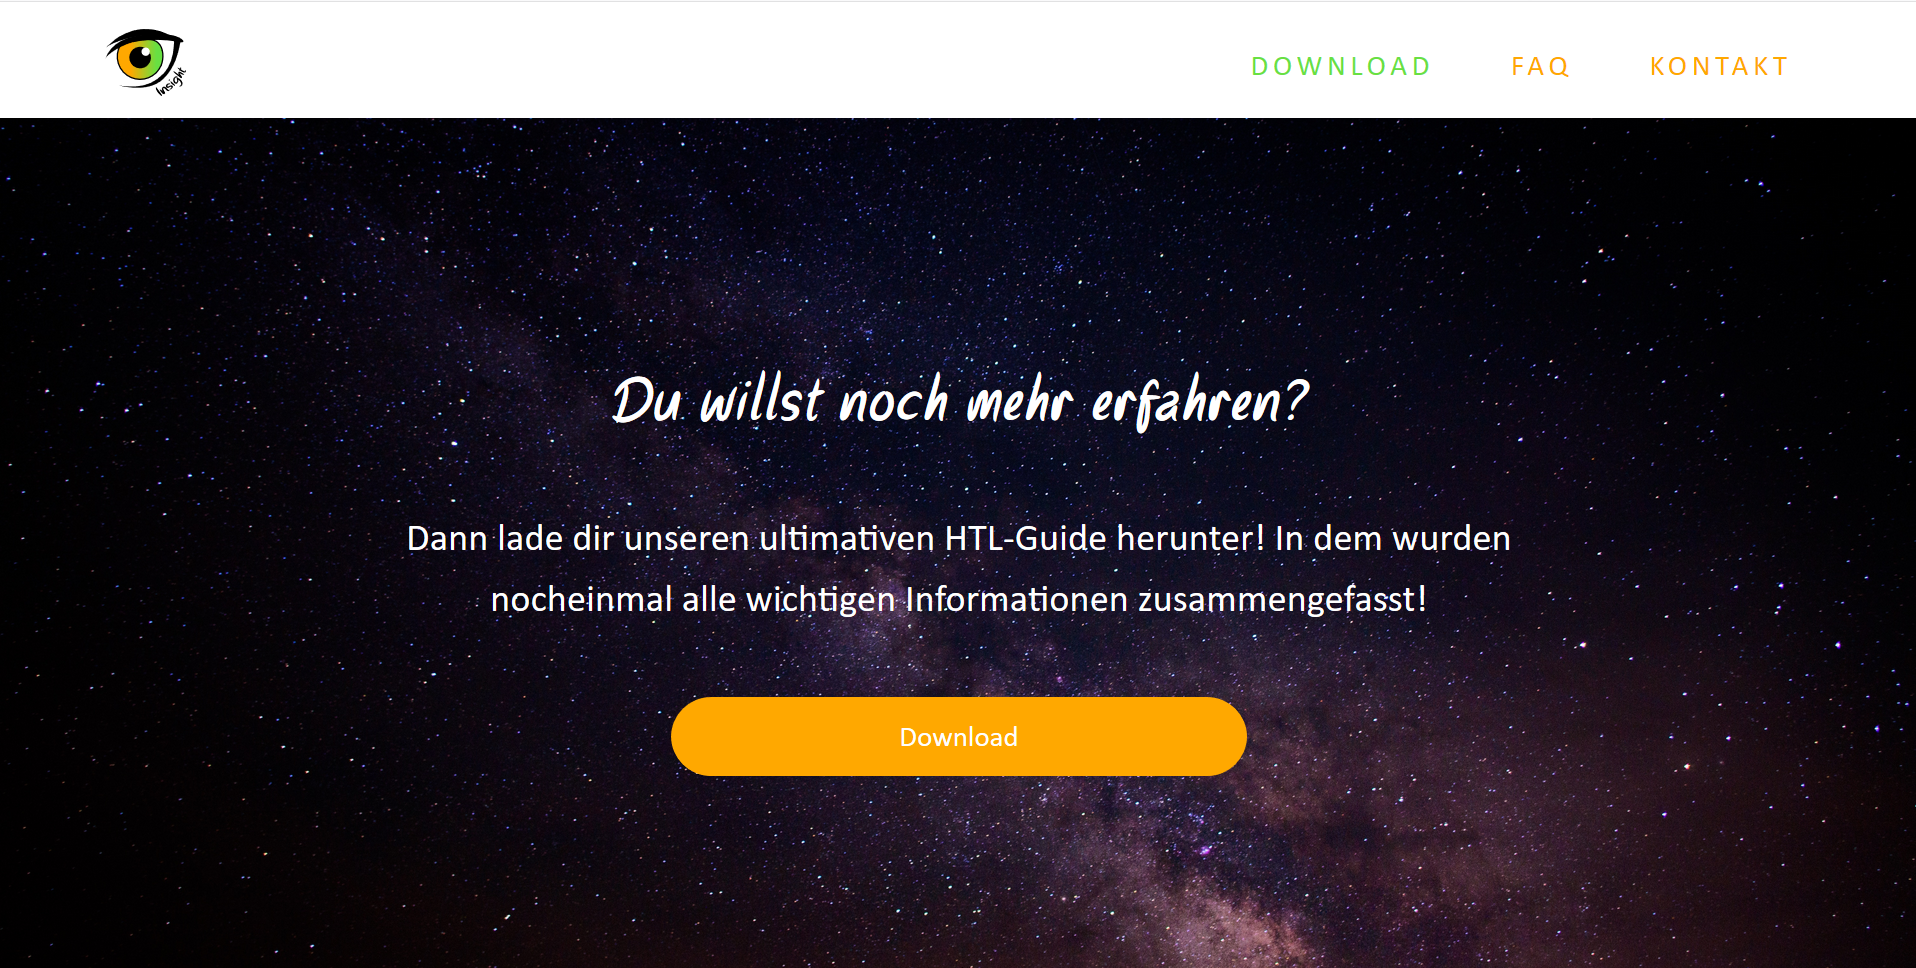
\includegraphics[width=12cm,height=12cm,keepaspectratio]{webseite_abb6} 
	\caption{Die Downloadseite}
	\label{Abb6}
\end{figure}
\paragraph{FAQ} \leavevmode \\
Der User hat die Möglichkeit, in das FAQ (Frequently Asked Questions) einen Blick zu werfen, auf der sich häufig gestellte Fragen befinden. Somit entlastet man diejenige Person, die sich um Fragen, die an die Schule gerichtet sind, kümmert. Die Fragen wurden am Tag der offenen Tür gesammelt und auch selbst ausgedacht. 
\begin{figure}[h]
	\centering				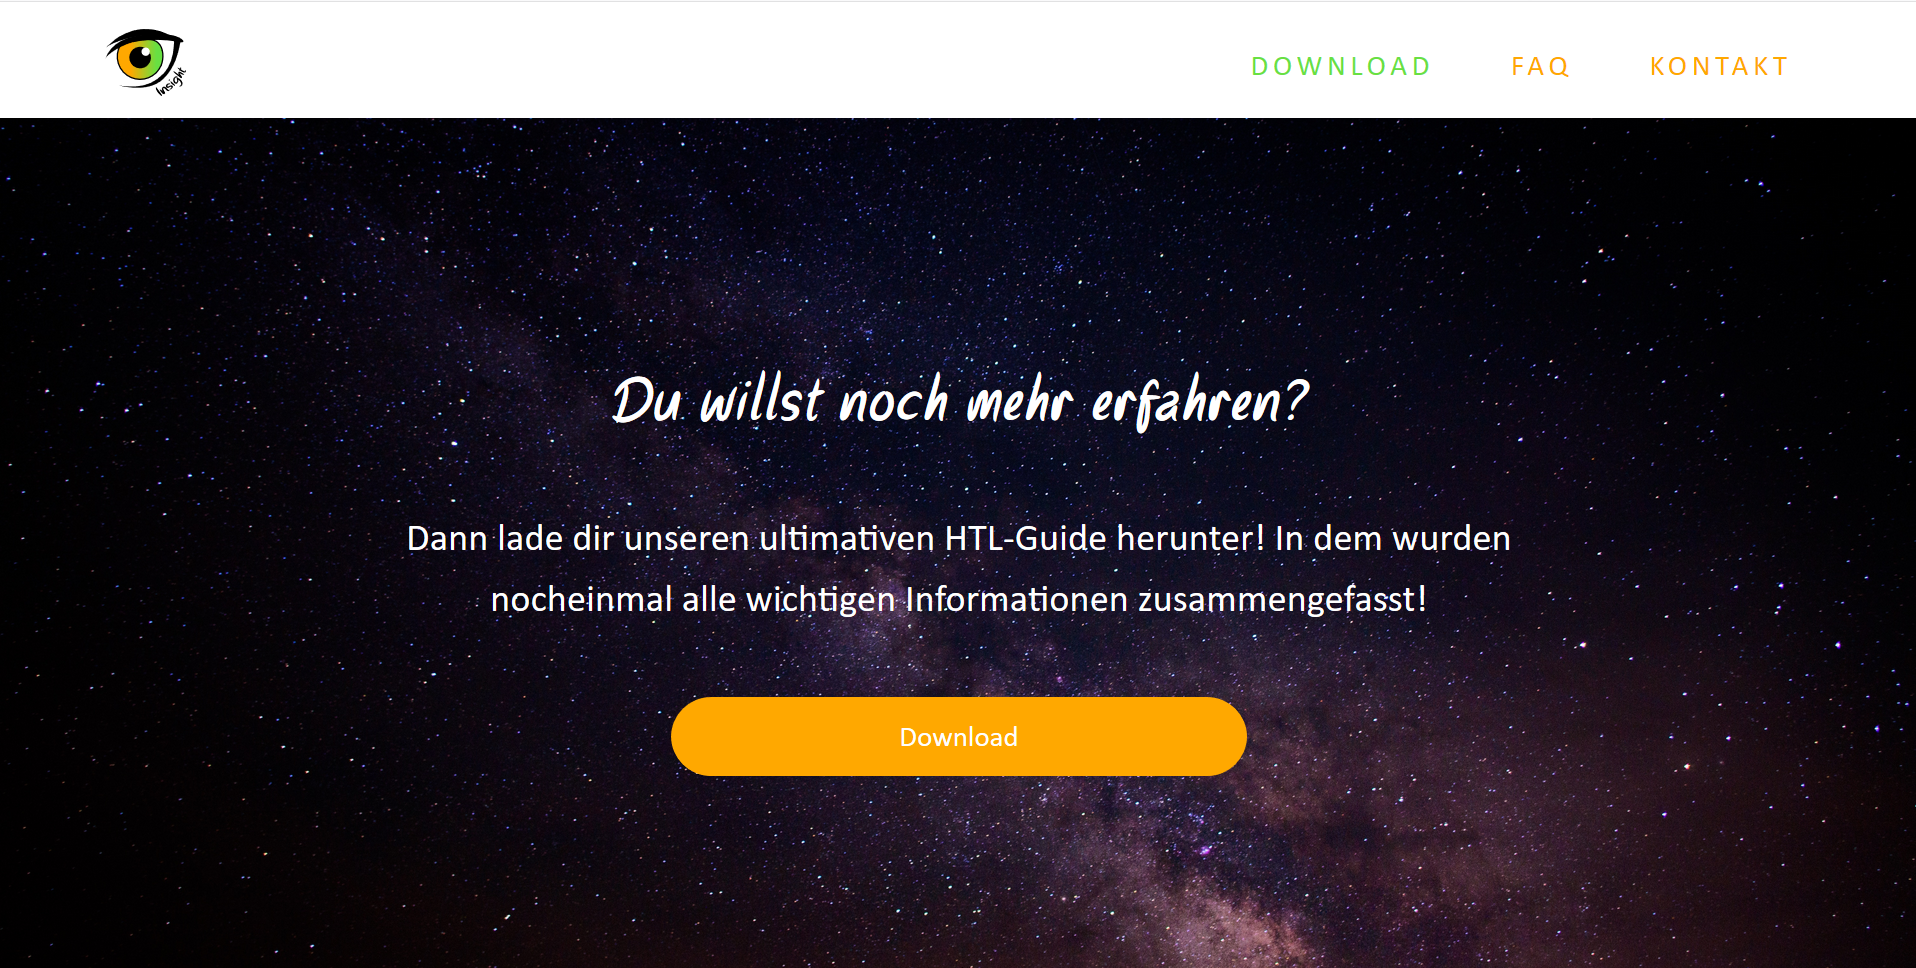
\includegraphics[width=12cm,height=12cm,keepaspectratio]{webseite_abb6} 
	\caption{Ein Platzhalter}
	\label{Abb7}
\end{figure} \leavevmode \newpage
\paragraph{Kontakt} \leavevmode \\
Falls die Fragen trotz der FAQ Seite nicht beantwortet werden konnten, kann auf die Kontaktseite gewechselt werden, welches ein Kontaktformular enthält, was das Kontaktieren der Schule vereinfachen soll.
Das Team hat eine eigene E-Mail-Adresse erstellt, welches die ausgefüllten Kontaktformulare geschickt bekommt. Dabei wurde das Service von formular-chef.de genutzt. Außerdem befinden sich auf dieser Seite auch Kontaktinformationen der Schule, falls es User präferieren die HTL anzurufen.
\begin{figure}[hb]
	\centering				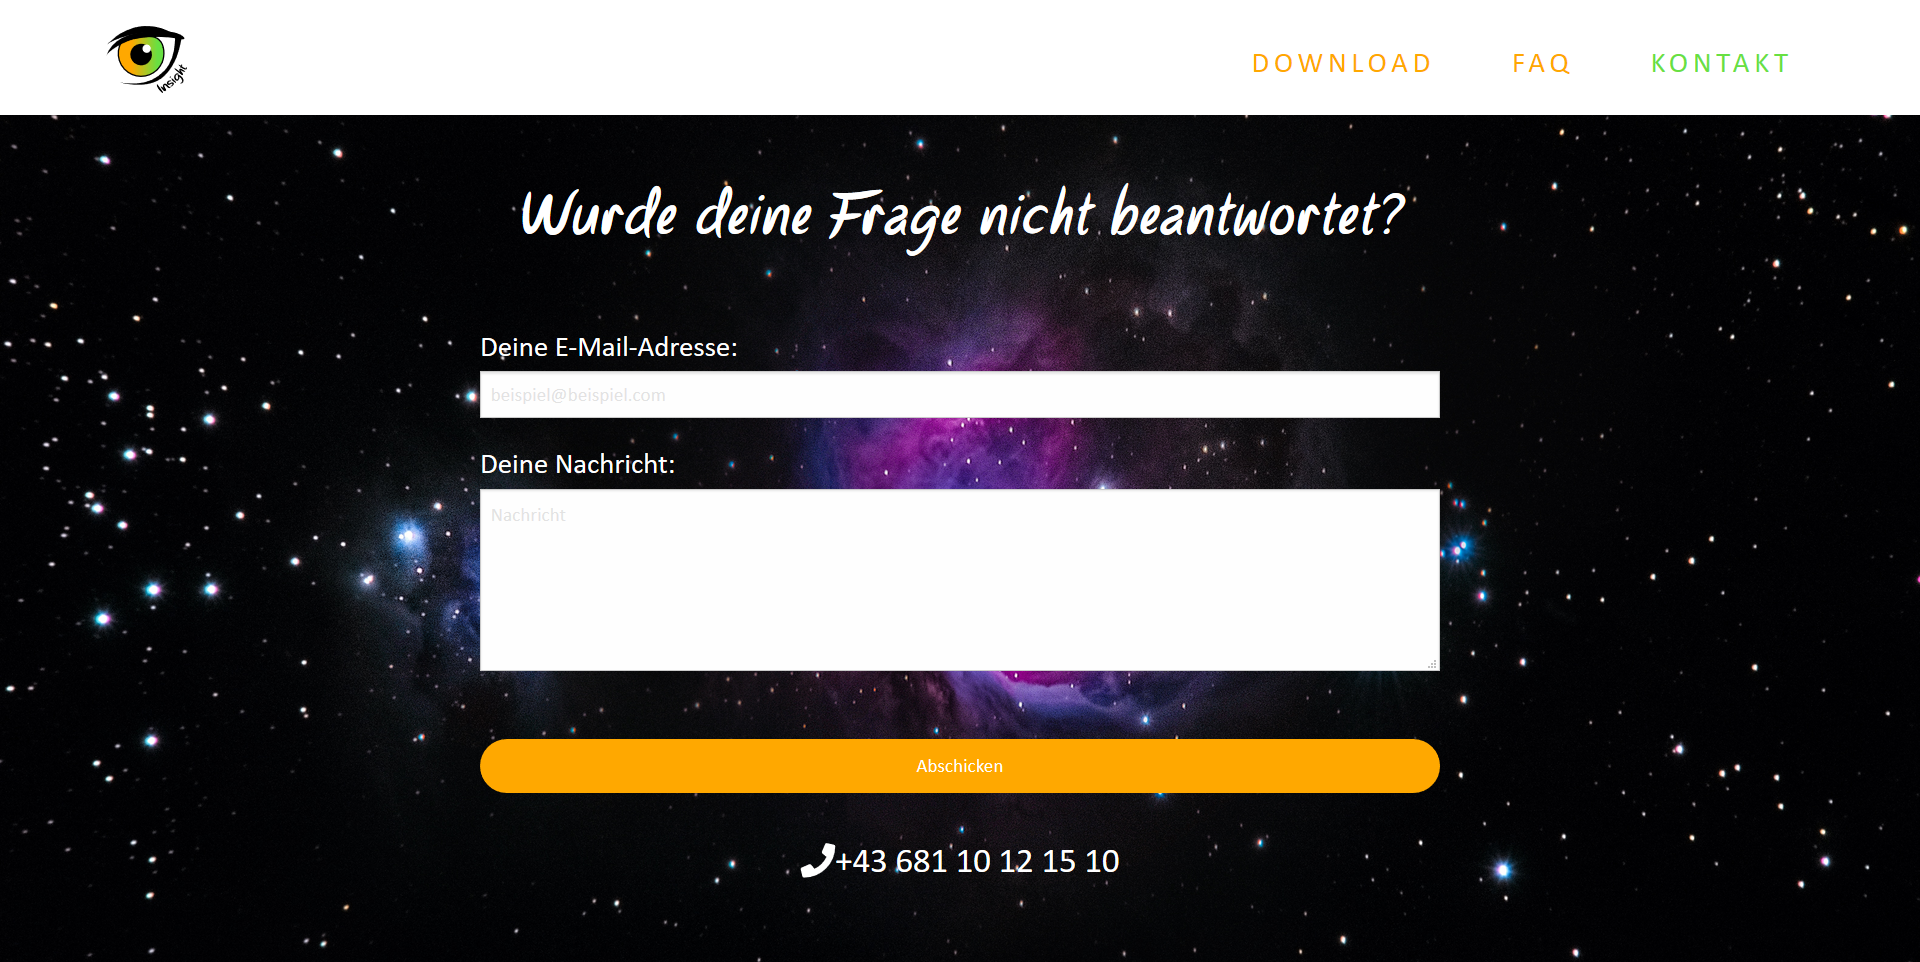
\includegraphics[width=12cm,height=12cm,keepaspectratio]{webseite_abb7} 
	\caption{Die Kontaktseite}
\end{figure} \leavevmode \newline
\section{Storytelling} 
\begin{quote}
“Kinder verpacken Ihre Ideen und Gedanken oftmals in Geschichten, um uns Erwachsene damit ihre Welt zu erklären. Als Erwachsene wiederum müssen wir es wieder lernen, Geschichten zu erzählen.“   \cite{storytellingzitat}
\end{quote}
Storytelling vermittelt durch den Einsatz von Geschichten Information. Die Geschichten können real oder konstruiert sein, es muss lediglich gut ankommen und im Kopf der Nutzer bleiben. Weiters dient Storytelling dazu, die Aufmerksamkeit des Nutzers auf eine kreative Weise zu ergattern. Die Informationen werden dabei anschaulich gemacht, um die Botschaft ankommen zu lassen. Wichtig ist die Erstellung eines oder mehreren Protagonisten und einem Problem. Im Laufe der Geschichte soll sich das Problem lösen, aber das muss nicht unbedingt sein. Eine gute Geschichte führt dazu, dass sich die Nutzer mit der Thematik auseinandersetzen und emotional aufgeladen sind. Weiters sorgt eine gute Story für Begeisterung. Es gibt verschiedene Arten von Storytelling, welche sich von Büchern bis hin zu Webseiten erstreckt. Das Internet bietet hier eine große Möglichkeit für das Erzählen von Geschichten. Wichtig ist vor allem die Interaktivität, damit es nicht zu schnell langweilig wird.  Für das Team war es wichtig, die Zielgruppe durch die Geschichte zu erreichen. Dabei sollten Klischees vermieden werden und die Nutzer sollten sich mit dem Erzähler identifizieren können. \cite{storytelling}
\subsection{Story}
Project Insight benutzt klassische Storytelling-Methoden, um Nutzer über die Medientechnik zu informieren. Dabei dachte sich das Team die Figur, Rene Weg, aus. Dieser ist ein Absolvent der HTL Rennweg und hat dem Nutzer gegenüber eine Mentor-Funktion. Rene Weg ist eine sarkastische und humorvolle Figur, welcher dem Nutzer die Medientechnik, auf eine spielerische und lockere Art und Weise, präsentiert. Es war dem Team sehr wichtig, ein paar Witze in die Story einzubinden, um dem Nutzer das Gefühl zu geben, dass man an der HTL Rennweg auch Spaß haben kann. Durch verschiedenste Gestiken und Mimik, wird Leben in die Figur gehaucht. \leavevmode \\
Abgesehen von der Rolle der Figur als Mentor, kommt sie auch noch in dem Animationsvideo (siehe Kapitel Animationsvideo) vor. 
\subsubsection{Aufbau}
Die Story ist in zehn Lektionen aufgeteilt. Dabei arbeitet sich der User stufenweise in die Medientechnik ein. Es beginnt mit einer Einführung und geht Schritt für Schritt die vorgegebenen Bereiche der Medientechnik durch und endet anschließend mit einem humorvollen Video. Bevor die Story beginnt, wird der User darauf hingewiesen, dass die Webseite Audio beinhaltet. 
\begin{figure}[ht]
	\centering				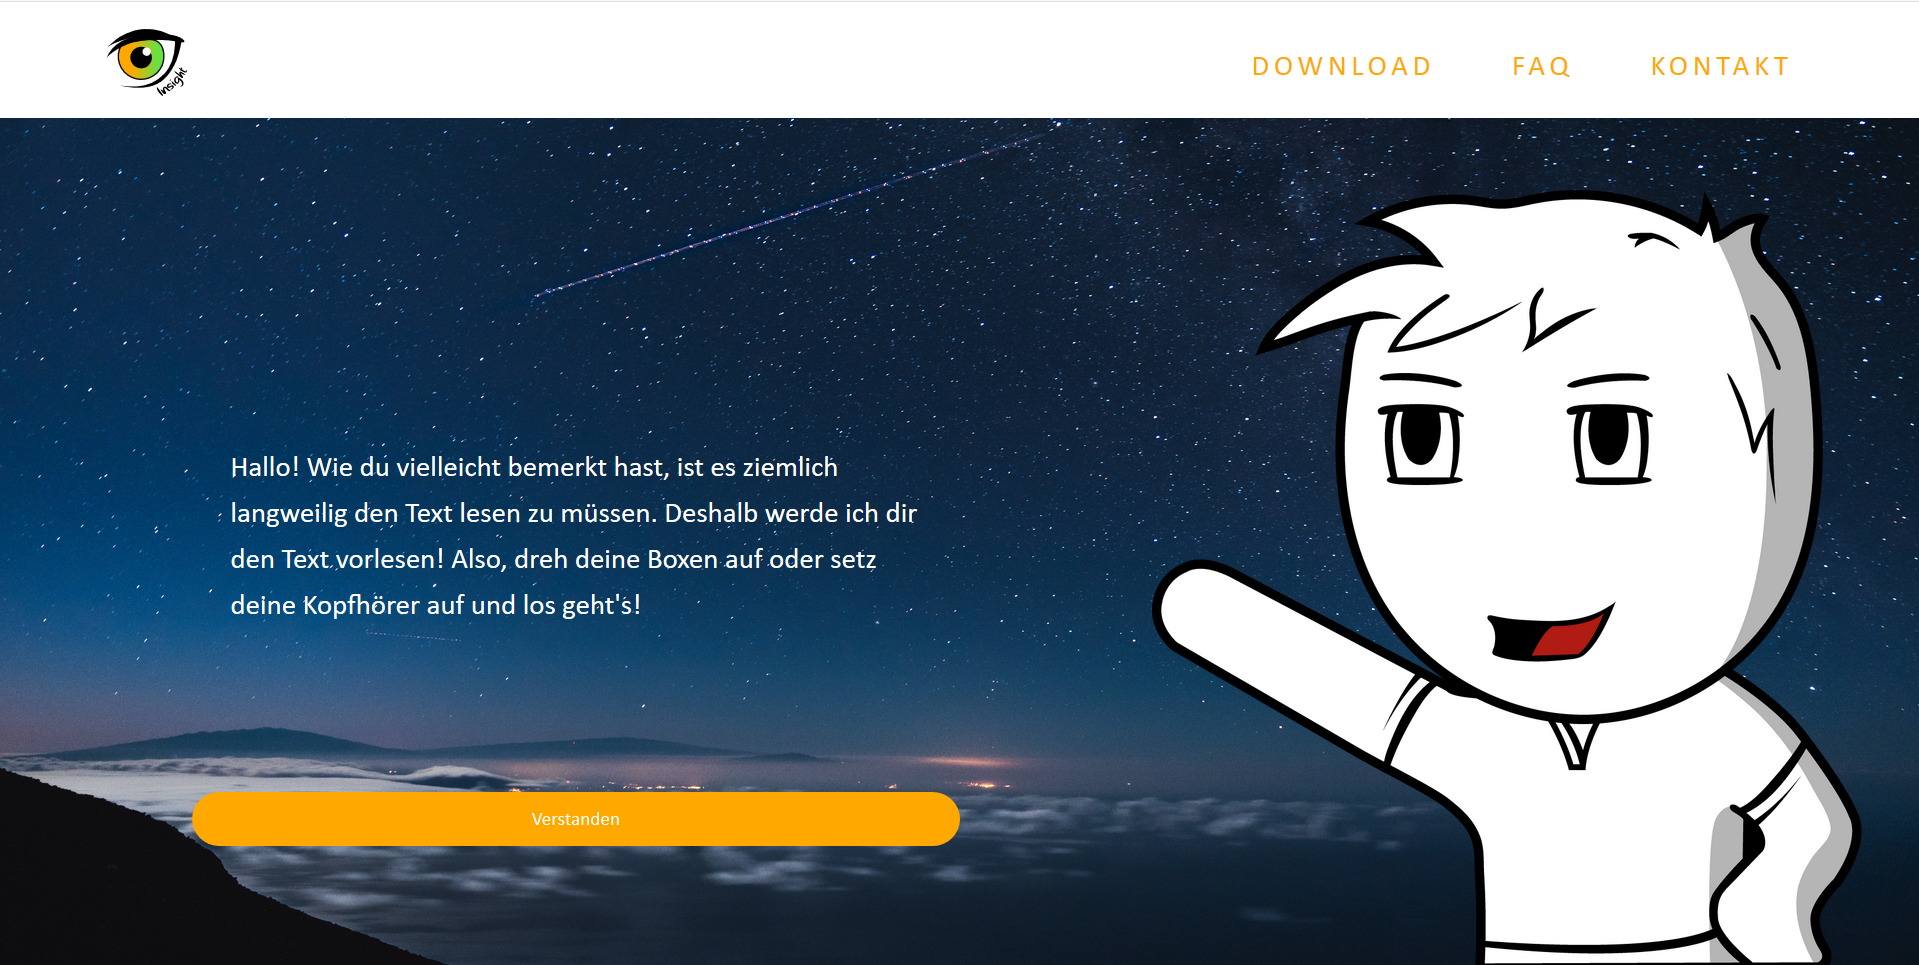
\includegraphics[width=12cm,height=12cm,keepaspectratio]{webseite_abb8} 
	\caption{Bevor die Lektion beginnt}
\end{figure} \leavevmode \newline
Die Webseite wird vom Charakter, Rene Weg, vertont. 
Für das Grundgerüst wurde das Framework Slick Slider verwendet. Dabei wurde eine Struktur erstellt, wo sich auf einer Seite der Text und auf der anderen Seite die Figur befindet. Zusätzlich befinden sich unter dem Text vier Buttons, welche für das Weiterschalten und für das Pausieren und Abspielen gedacht sind. \leavevmode \newpage
\lstset{
  frame=leftline,
  breaklines=true,
}
\begin{lstlisting}[language=HTML, basicstyle=\scriptsize]
 <div id="slide1" class="slide">
        <div class="left">
            <p class="text_mittig">Das war jetzt ziemlich viel &uuml;ber die HTL. Aber, du bist doch wegen der Medientechnik hier. Also, plaudern wir &uuml;ber die Medientechnik! </p>
	        <div id="groupofbuttons">
		        <a id="mute">
		        	<i class="fa fa-pause-circle"></i>
		        </a>
		        <a id="unmute">
		        	<i class="fa fa-play-circle"></i>
		        </a>
		        <a class="previous">
		        	<i class="fa fa-chevron-circle-left"></i>
		        </a>
		        <a class="next">
		        	<i class="fa fa-chevron-circle-right"></i>
		        </a>
	        </div>
        </div>
        <div class="right">
            <img src="../images/figuren/martin_normal.png" class="charakter">

        </div>

        <audio id="audio1" src="../audio/Lektion3_01.mp3" autoplay></audio>

</div>
\end{lstlisting}
 \leavevmode \\
Ein Slide wird durch die id "slide[nummer]" initialisiert. Dieses Slide beinhaltet zwei Div Boxen, welche sich jeweils rechts und links befinden. In der linken Div Box, mit der Klasse "left", befinden sich der Text, welches der Charakter spricht, sowie die Buttons zum Weiterschalten, Pausieren und Abspielen. In der rechten Div Box, mit der Klasse "right", ist die Figur mit ihren verschiedenen Gestiken zu sehen. Jeder neuen Geste, wurde eine neue CSS Klasse geschrieben, damit die Figur immer auf der selben Position steht.
\begin{figure}[h]
	\centering				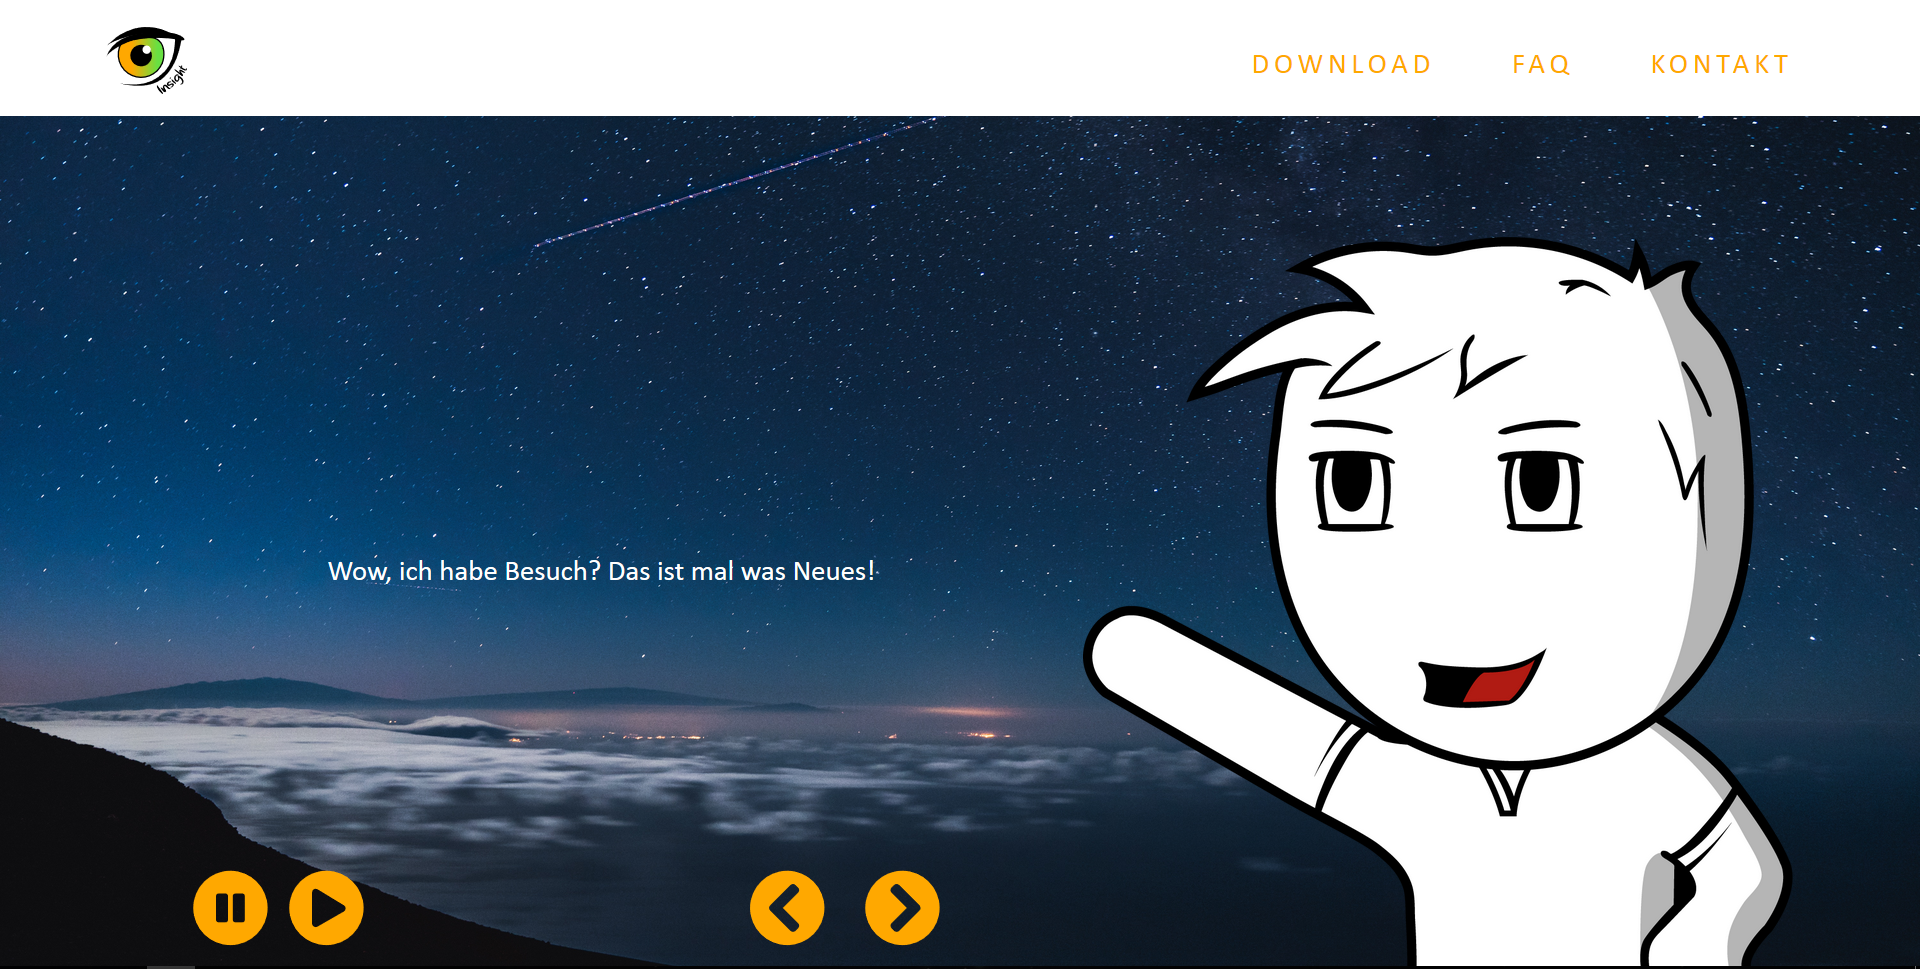
\includegraphics[width=12cm,height=12cm,keepaspectratio]{webseite_abb9} \leavevmode \newline 
	\caption{Aufbau der Lektionen}
	\label{AufbauLektionen}
\end{figure} \leavevmode \newline
Klickt man auf die Next und Previous Buttons, welche man in \ref{AufbauLektionen} sieht, kommt man zum nächsten Slide. Sobald man auf den Pause-Button klickt, wird das Audio pausiert und kann durch den Play-Button wieder abgespielt werden. Will man sich das Audio noch einmal anhören, so kann man ebenfalls auf den Play-Button klicken. Die große Problematik beim Aufbau war es, pro Slide ein einziges Audio-File abzuspielen. Öfters ist es vorgekommen, dass beim Weiterklicken, das vorherige Audio-File noch mitgespielt hat. Um dies zu verhindern, wurden if-Statements eingebaut, welche überprüfen, ob sich der User in einem bestimmten Slide befindet. Befindet sich der User beispielsweise im zweiten Slide, wird das zugehörige Audio-File abgespielt. Sobald man das zweite Slide verlässt, pausiert sich das Audio-File, sodass zwei oder mehrere Audio Files nicht gleichzeitig abgespielt werden. \leavevmode \\
Nicht jedes Slide hat ein Audio-File, da es Slides gibt, welche den User darüber informieren, welche Lektion gerade bearbeitet wird. Bei diesen Slides ändert sich die Struktur, denn die Play und Pause-Buttons verschwinden und die Buttons zum Weiterschalten rücken in die Mitte. Außerdem gibt es Slides, welche Videos beinhalten und ebenfalls keine Play und Pause-Buttons enthalten. Am Ende der Lektion wurde dem Weiterschalt-Button ein Link zur nächsten Lektion hinzugefügt.
\lstset{
  frame=leftline,
  xleftmargin=.05\textwidth
}
\begin{lstlisting}
if (slick.$slides.length-1 === currentSlide) {
	$('.next').click(function(){
    	$('.next').attr('href', 'lektion_4.html');
    });
}
\end{lstlisting} \leavevmode \newline
Hierbei wird der letzte Slide ermittelt und den Buttons zum Weiterschalten ein Link hinzugefügt. Durch diese Methode, muss pro HTML-Dokument nur der Link zum nächsten HTML-Dokument angegeben werden. \leavevmode \\
In den folgenden Absätzen, werden alle Lektionen zusammengefasst. 
\paragraph{Lektion 1}\leavevmode \\
In der ersten Lektion wird der Charakter, Rene Weg, vorgestellt. Nachdem er sich humorvoll vorgestellt hat, werden Fragen rund um die HTL beantwortet. Um dies veranschaulichen zu können, wird ein Animationsvideo vorgeführt. Die erste Lektion dient nur als Einführung in eine HTL und soll die User mit Rene Weg bekannt machen. 
\begin{figure} [h]
	\centering
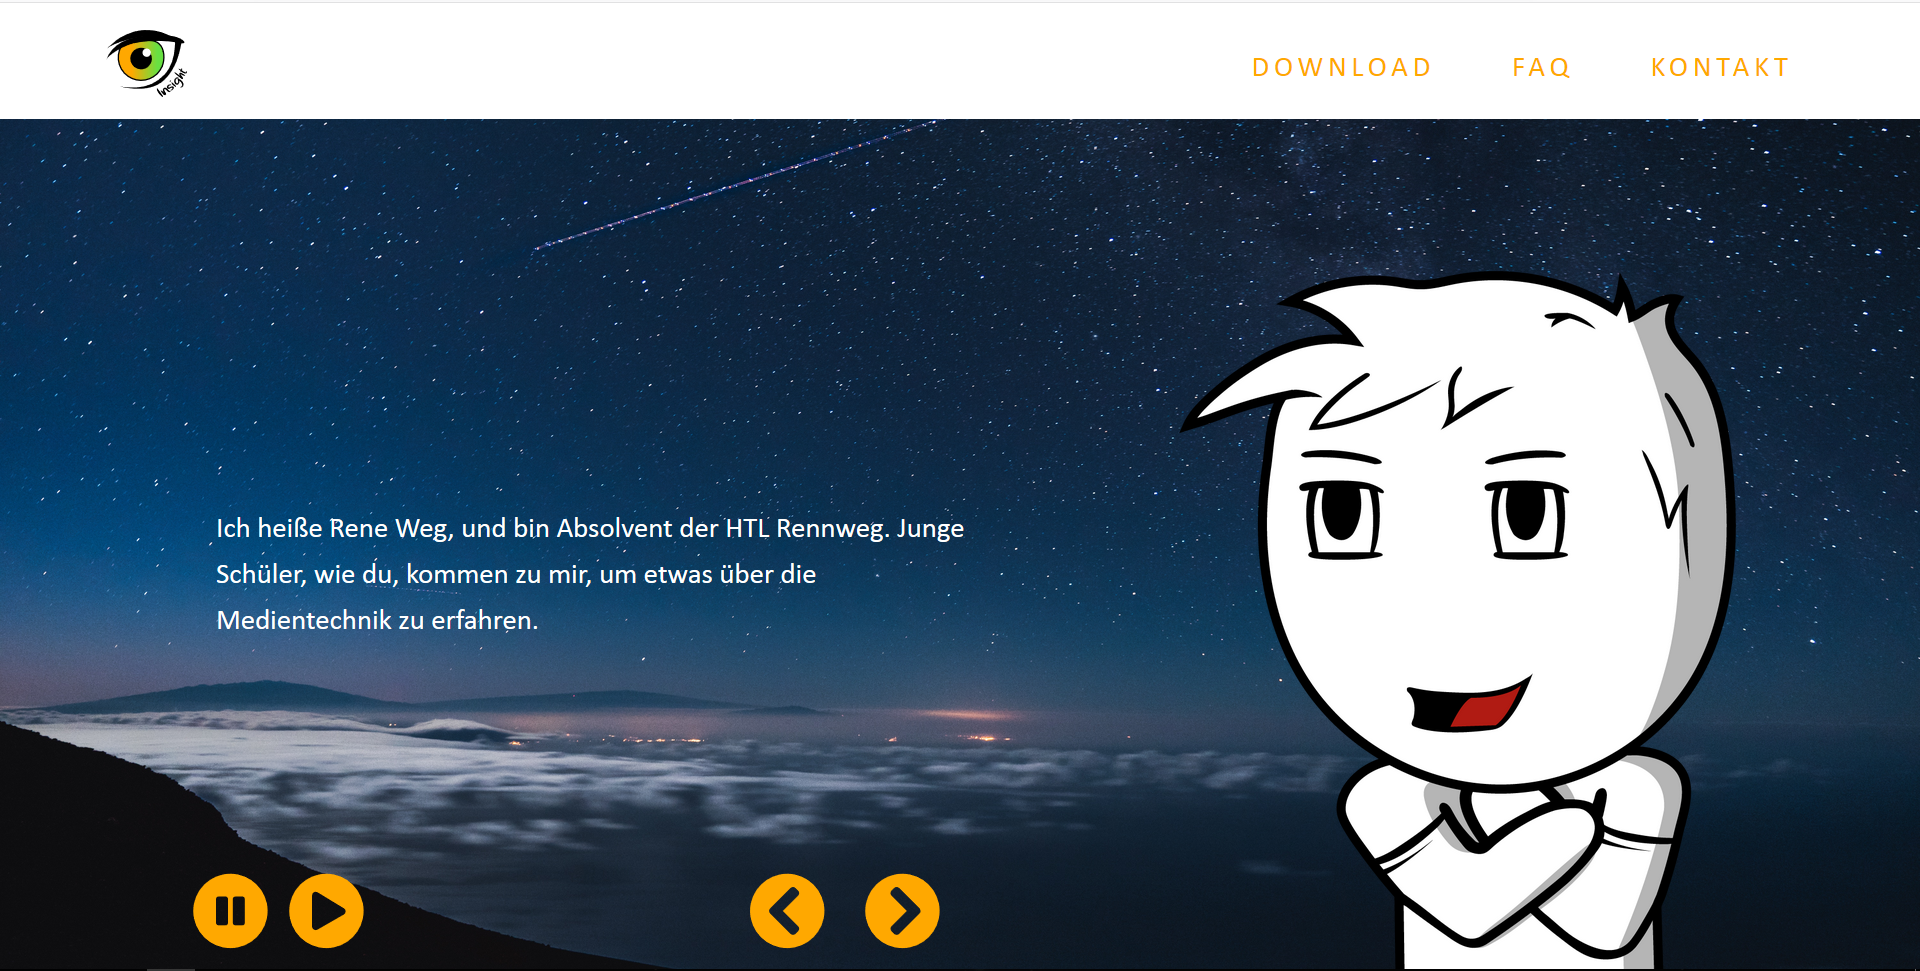
\includegraphics[width=12cm,height=12cm,keepaspectratio]{webseite_abb12} 
	\caption{Der Anfang}
\end{figure}
\paragraph{Lektion 2} \leavevmode \\
Da die HTL etwas Neues für die User ist und sie nicht wissen, was ein Abteilungsvorstand ist, geht es in der zweiten Lektion um ihn. Dabei wird erklärt, was ein Abteilungsvorstand ist. Außerdem wird ein Interview mit dem Abteilungsvorstand der HTL Rennweg, Dr. Gerhard Hager, gezeigt. 
\begin{figure} [h]
	\centering
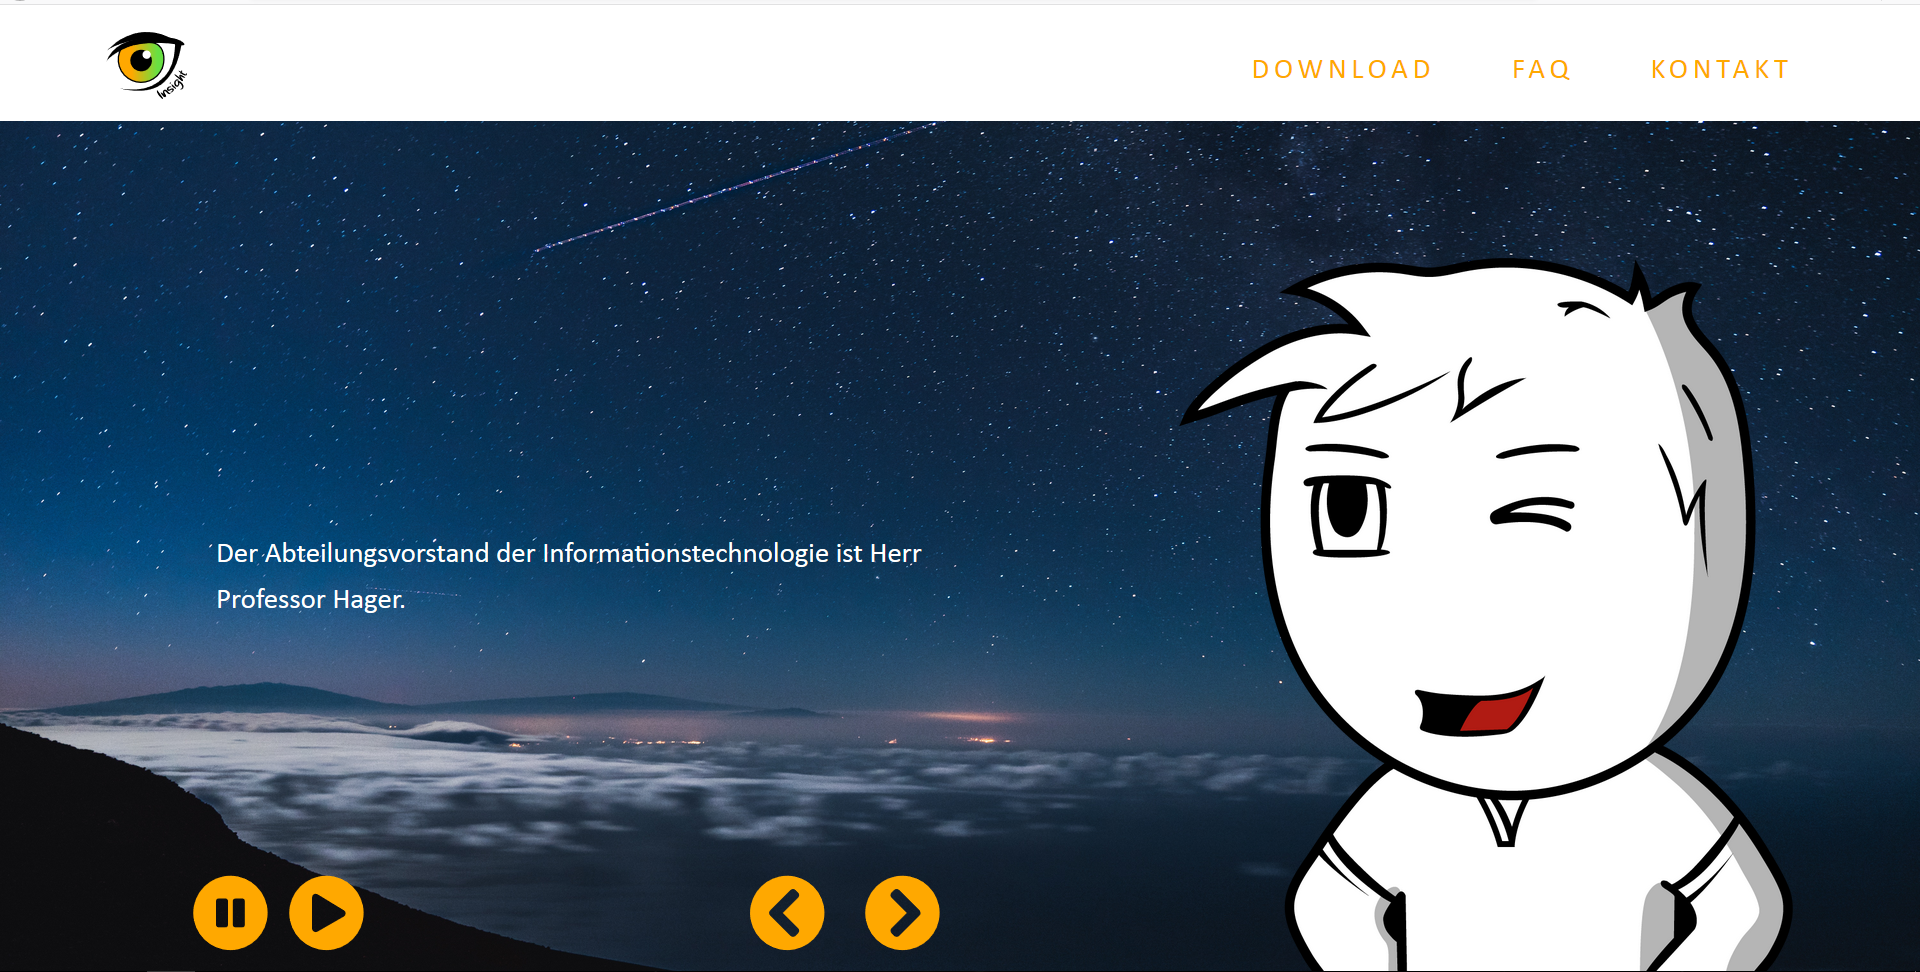
\includegraphics[width=12cm,height=12cm,keepaspectratio]{webseite_abb13} 
	\caption{Der Abteilungsvorstand}
\end{figure}
\paragraph{Lektion 3} \leavevmode \\
Wenn man im Internet nach der Medientechnik recherchiert, findet man komplexe Erklärungen, die sich teilweise widersprechen. Aus dem Grund, hat sich das Team dazu entschlossen in der dritten Lektion die Medientechnik zu erklären. Diese Lektion ist die einzige Lektion, in der es keine interaktiven Elemente gibt. Rene Weg vergleicht dabei die Größe der Medientechnik, mit der des Universums und bezieht sich somit auf das „Space-Theme“. 
\begin{figure} [h]
	\centering
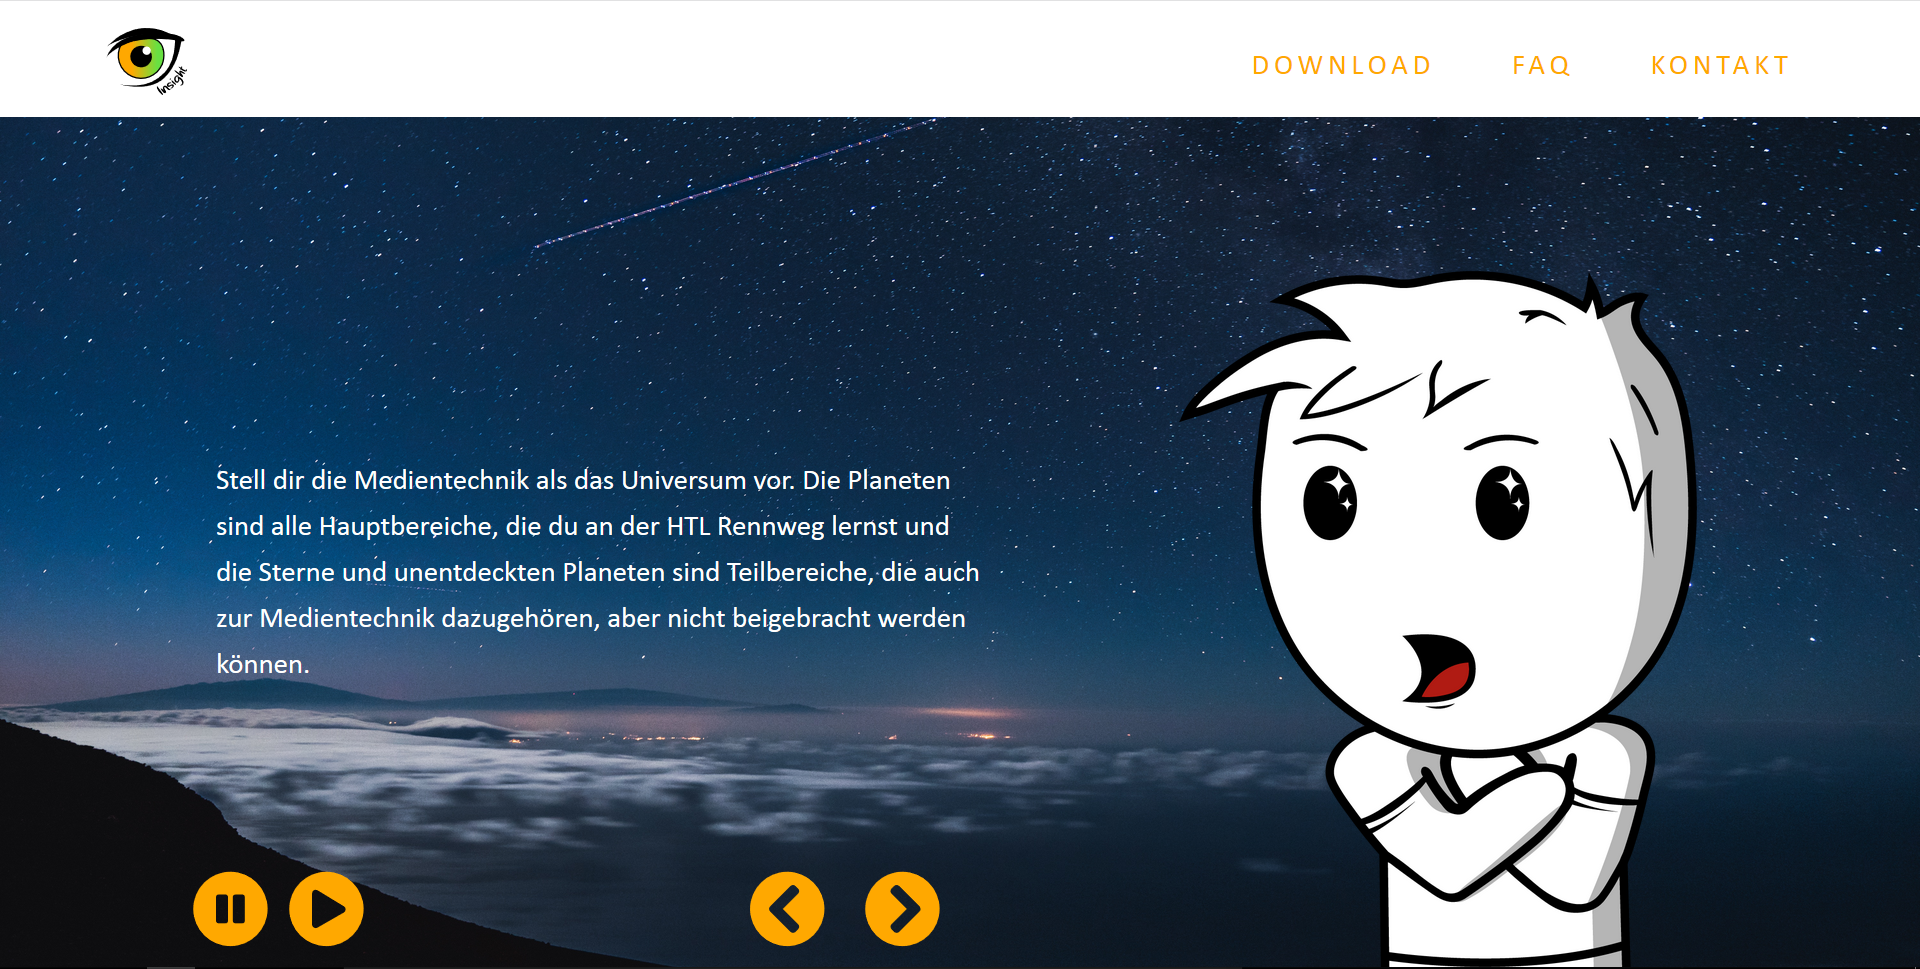
\includegraphics[width=12cm,height=12cm,keepaspectratio]{webseite_abb14} 
	\caption{Die Medientechnik}
\end{figure}
\paragraph{Lektion 4} \leavevmode \\
Mediengestaltung spielt eine große Rolle und wird in der vierten Lektion behandelt. Dabei erklärt Rene Weg dem User, wie wichtig es ist, langweiligen Inhalt spannend zu gestalten. Als Beispiel wird die Entstehungsgeschichte der HTL aufgelistet und danach wird eine spannendere Auflistung hergezeigt. Dieses Kapitel dient dazu, dem User zu zeigen, wie wichtig Kreativität in der Medientechnik ist und, dass man mit seinem Inhalt hervorstechen muss, um erfolgreich zu sein.
\begin{figure} [h]
	\centering
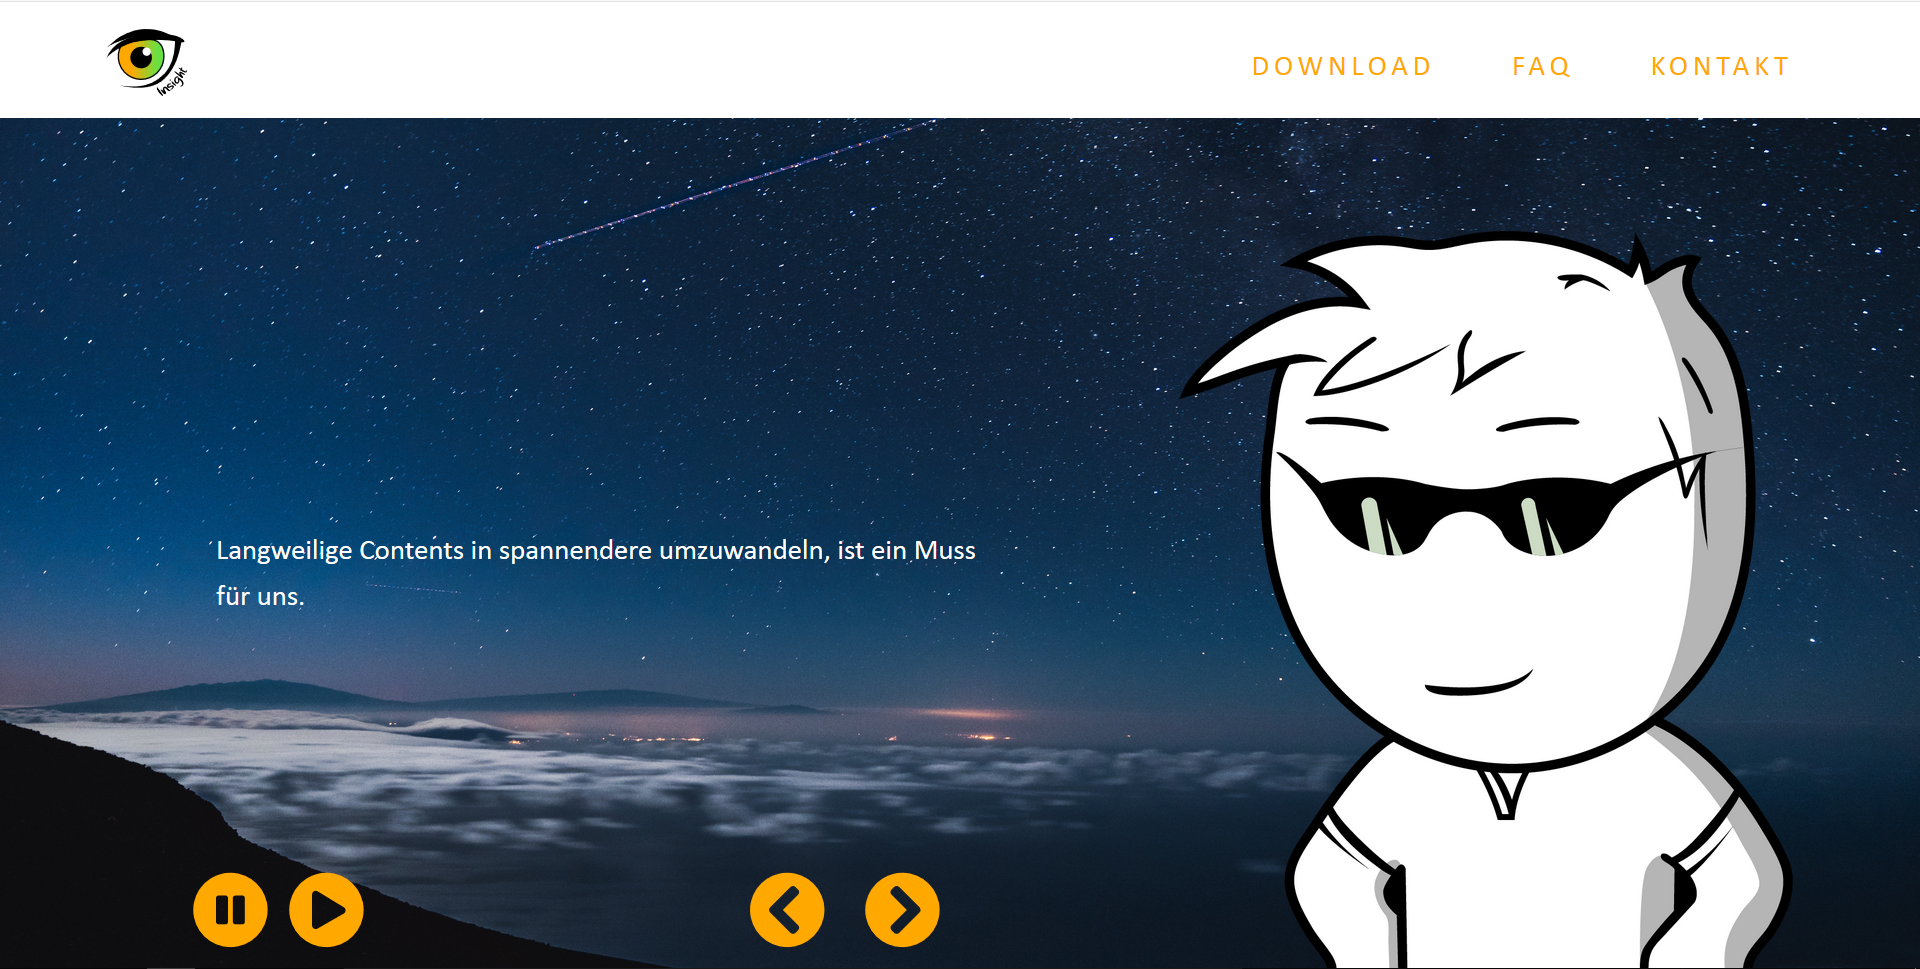
\includegraphics[width=12cm,height=12cm,keepaspectratio]{webseite_abb15} 
	\caption{Kreativität}
\end{figure}
\paragraph{Lektion 5} \leavevmode \\
Spiele sind sehr populär und werden in der fünften Lektion behandelt. Viele Interessenten interessieren sich für die Entwicklung von Spielen und sehen ein paar bei den Diplomarbeiten am Tag der offenen Tür. Das Team hat sich dabei dazu entschieden, den Code herzuzeigen. Damit der Code kurz und knapp ist und nicht zu kompliziert wirkt, da die User keine Erfahrung damit gemacht haben, hat sich das Team für das Spiel Memory entschieden. Nachdem der Code gezeigt wird, kann der User das Spiel auch spielen.
\begin{figure} [h]
	\centering
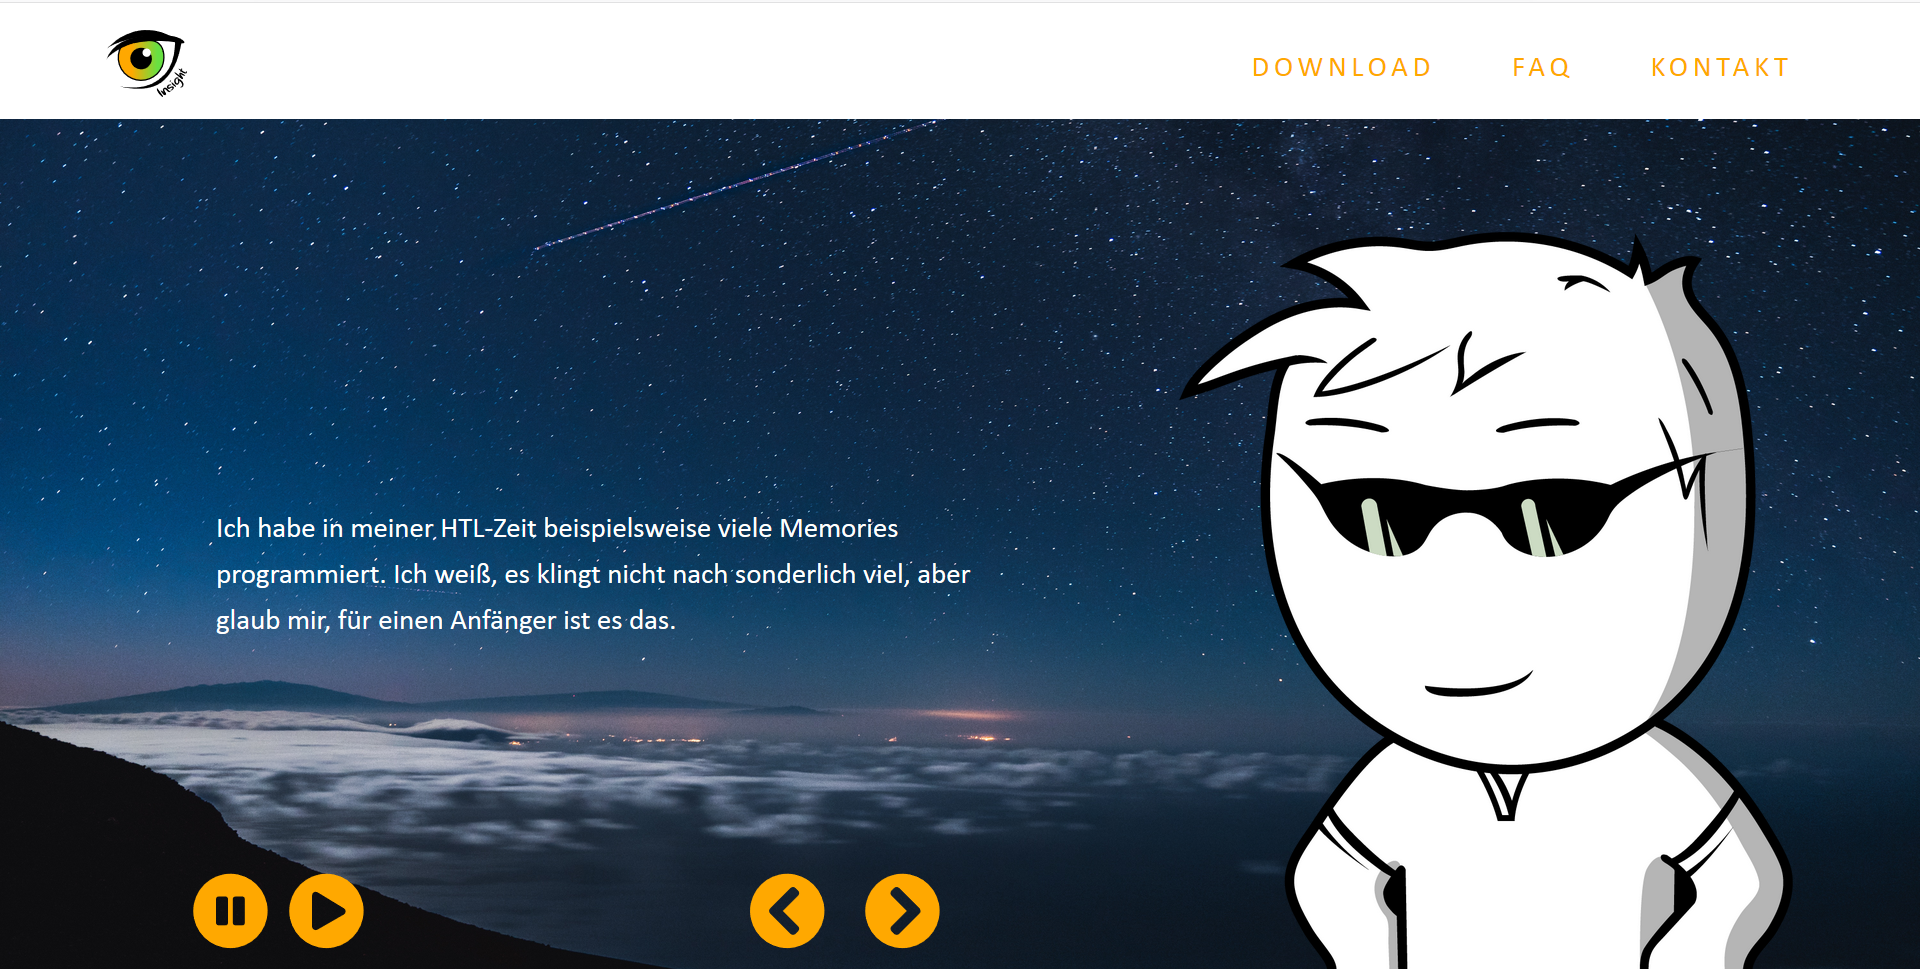
\includegraphics[width=12cm,height=12cm,keepaspectratio]{webseite_abb16} 
	\caption{Das Memory Spiel}
\end{figure}
\paragraph{Lektion 6} \leavevmode \\
Eine Animation muss sich nicht immer flüssig bewegen. Um dem User zu zeigen, was Animationen sind, werden diese in der sechsten Lektion behandelt. Rene Weg bezieht sich dabei auch auf das Animationsvideo, welches in der ersten Lektion gezeigt wurde. Als interaktives Element kann der User ein eigenes Universum kreieren, in dem es die vordefinierten Planeten verschiebt. 
\begin{figure} [h]
	\centering
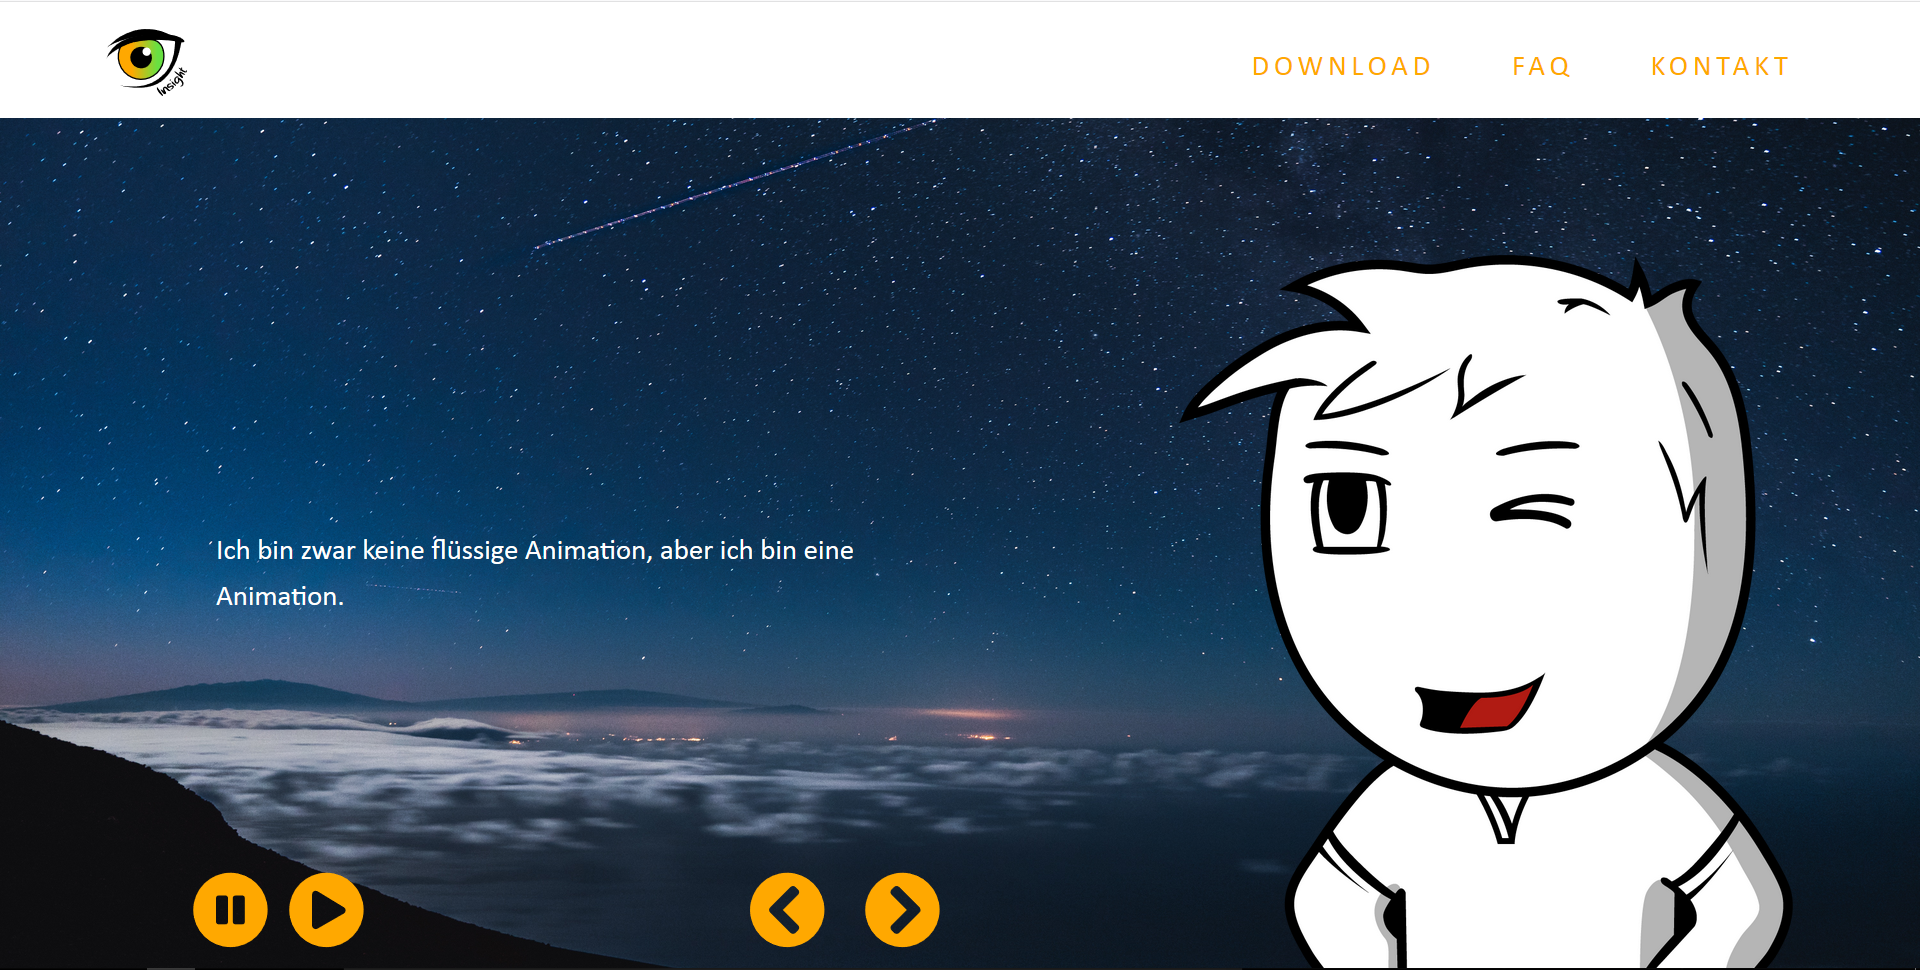
\includegraphics[width=12cm,height=12cm,keepaspectratio]{webseite_abb17} 
	\caption{Die Animationen}
\end{figure}
\paragraph{Lektion 7} \leavevmode \\
In der siebten geht es um Schrödingers Katze. Die Idee dahinter war, eine beliebte Referenz einer Fernsehserie, in ein interaktives Element umzuwandeln. In der Fernsehserie, The Big Bang Theory, gibt es eine Folge, in der Schrödingers Katze erwähnt wird und diese Folge ist sehr populär. Dies nahm das Team als Inspiration und programmierte eine Kiste, die geschlossen zu sein scheint. Fährt man mit der Maus über die Kiste, so sieht man eine weiße Katze. Dieses Kapitel unterstreicht, dass Kreativität sehr wichtig in der Medientechnik ist.
\begin{figure} [h]
	\centering
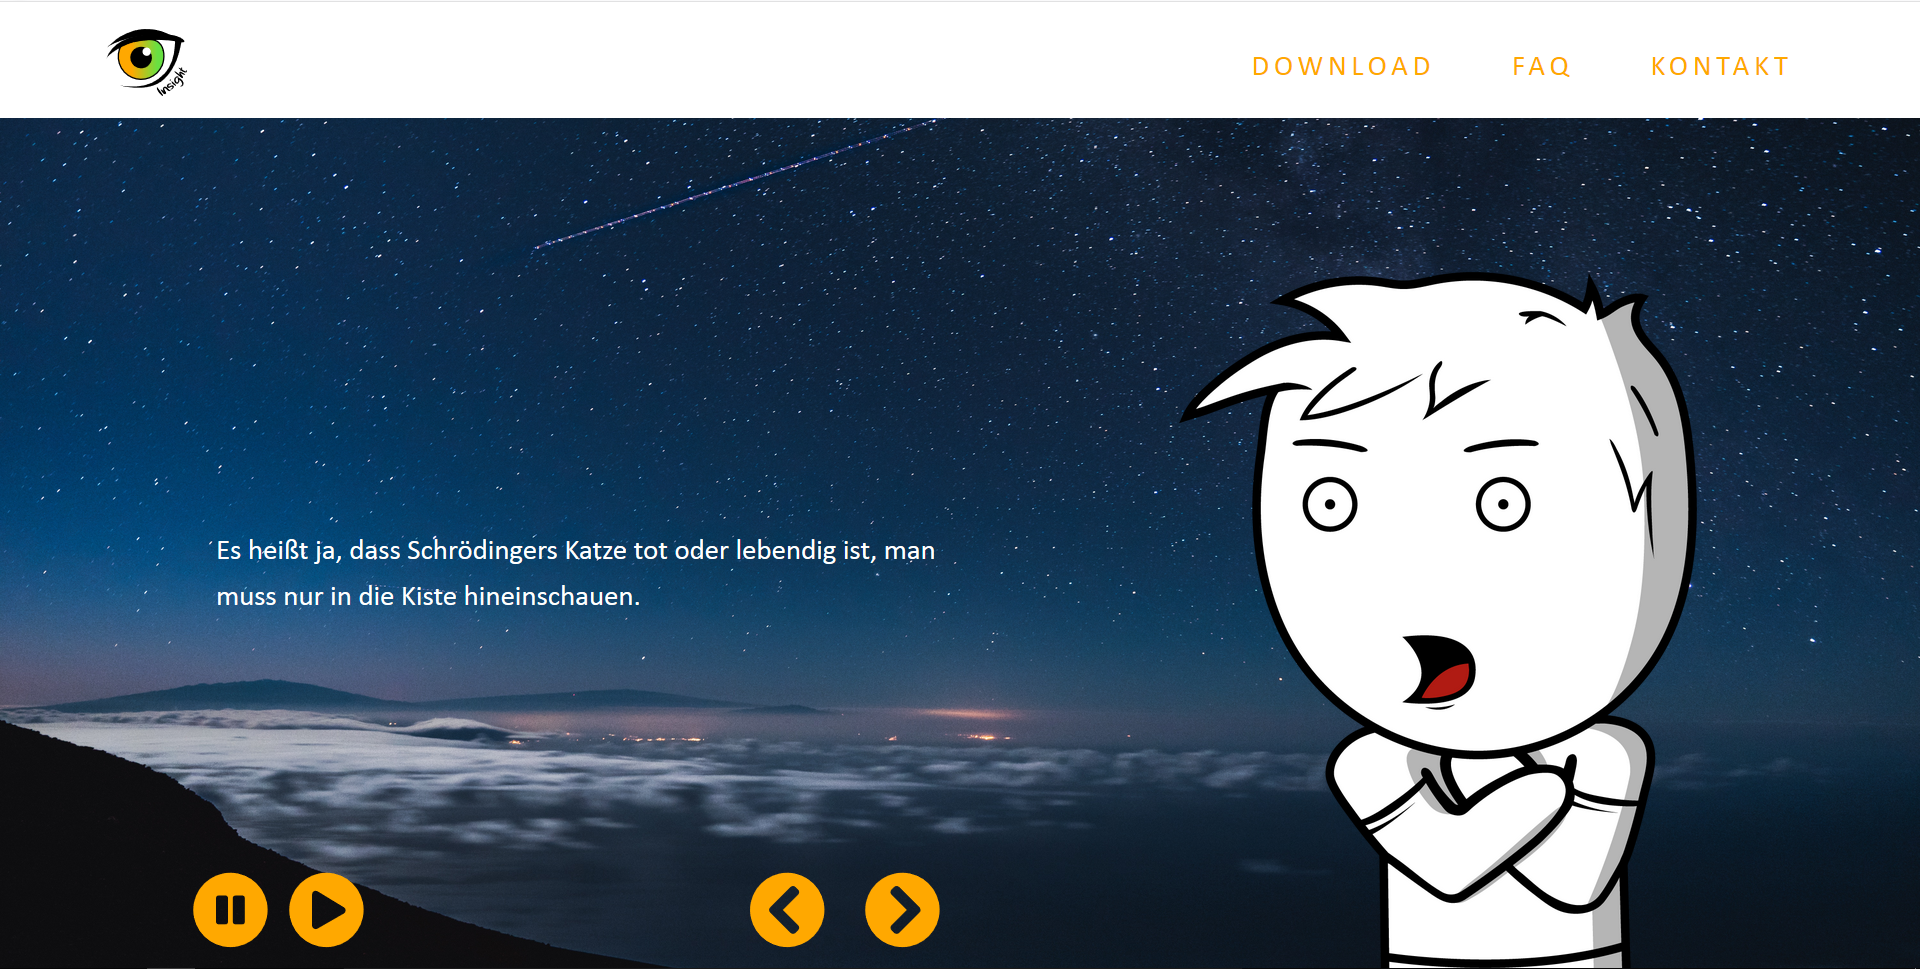
\includegraphics[width=12cm,height=12cm,keepaspectratio]{webseite_abb18} 
	\caption{Schrödingers Katze}
\end{figure}
\paragraph{Lektion 8} \leavevmode \\
Es gibt immer mehr Dienste im Internet, welche es ermöglichen eine Webseite zu erstellen. Das bringt natürlich die Frage auf, ob man die HTL braucht, wenn man alles im Internet findet und dort lernen kann. Dafür hat das Diplomarbeitsteam den Medientechniklehrer und Medientechnikfachmann, Mag. Roman Jerabek, interviewt. In dem Interview wird die Medientechnik besprochen und ihre Wichtigkeit hinterfragt.
\begin{figure} [h]
	\centering
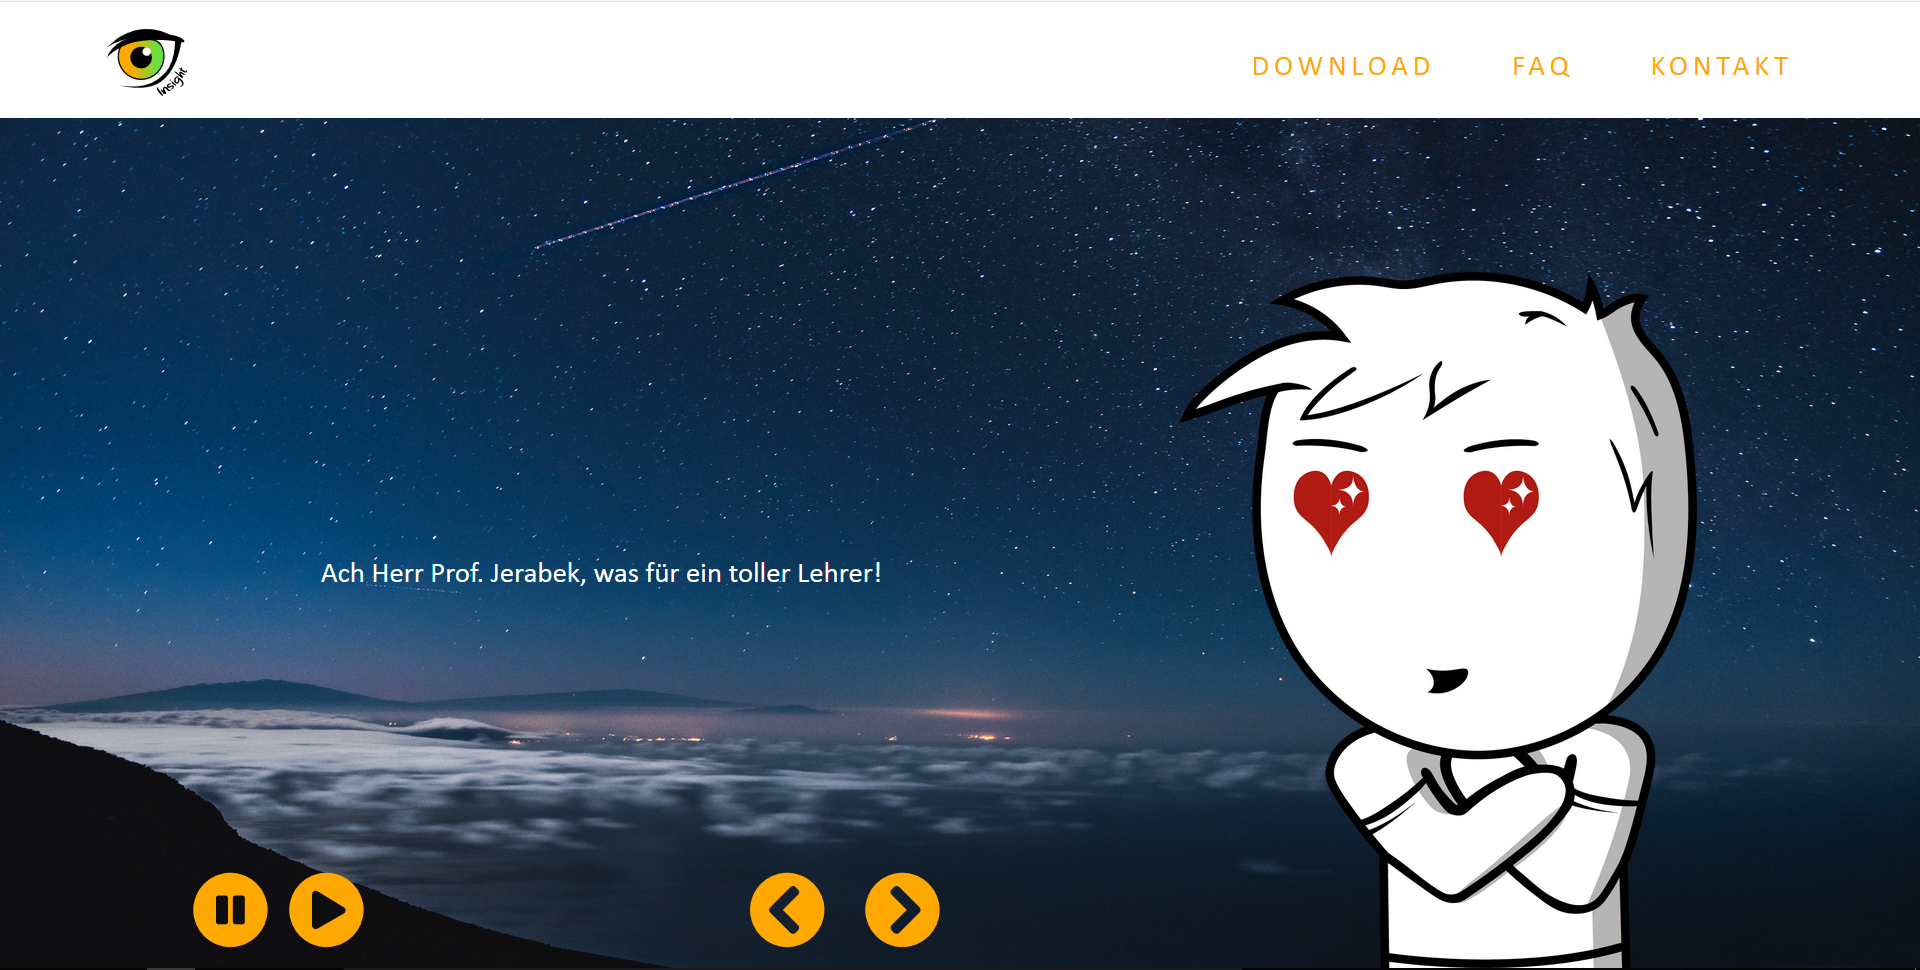
\includegraphics[width=12cm,height=12cm,keepaspectratio]{webseite_abb19} 
	\caption{Der Medientechniklehrer}
\end{figure}
\paragraph{Lektion 9} \leavevmode \\
In der neunten Lektion können User sehen, was andere Interessenten über die Schule denken. Dies soll dazu dienen, die Entscheidung der User zu erleichtern, da sie die Meinung von anderen Interessenten hören.
\begin{figure} [h]
	\centering
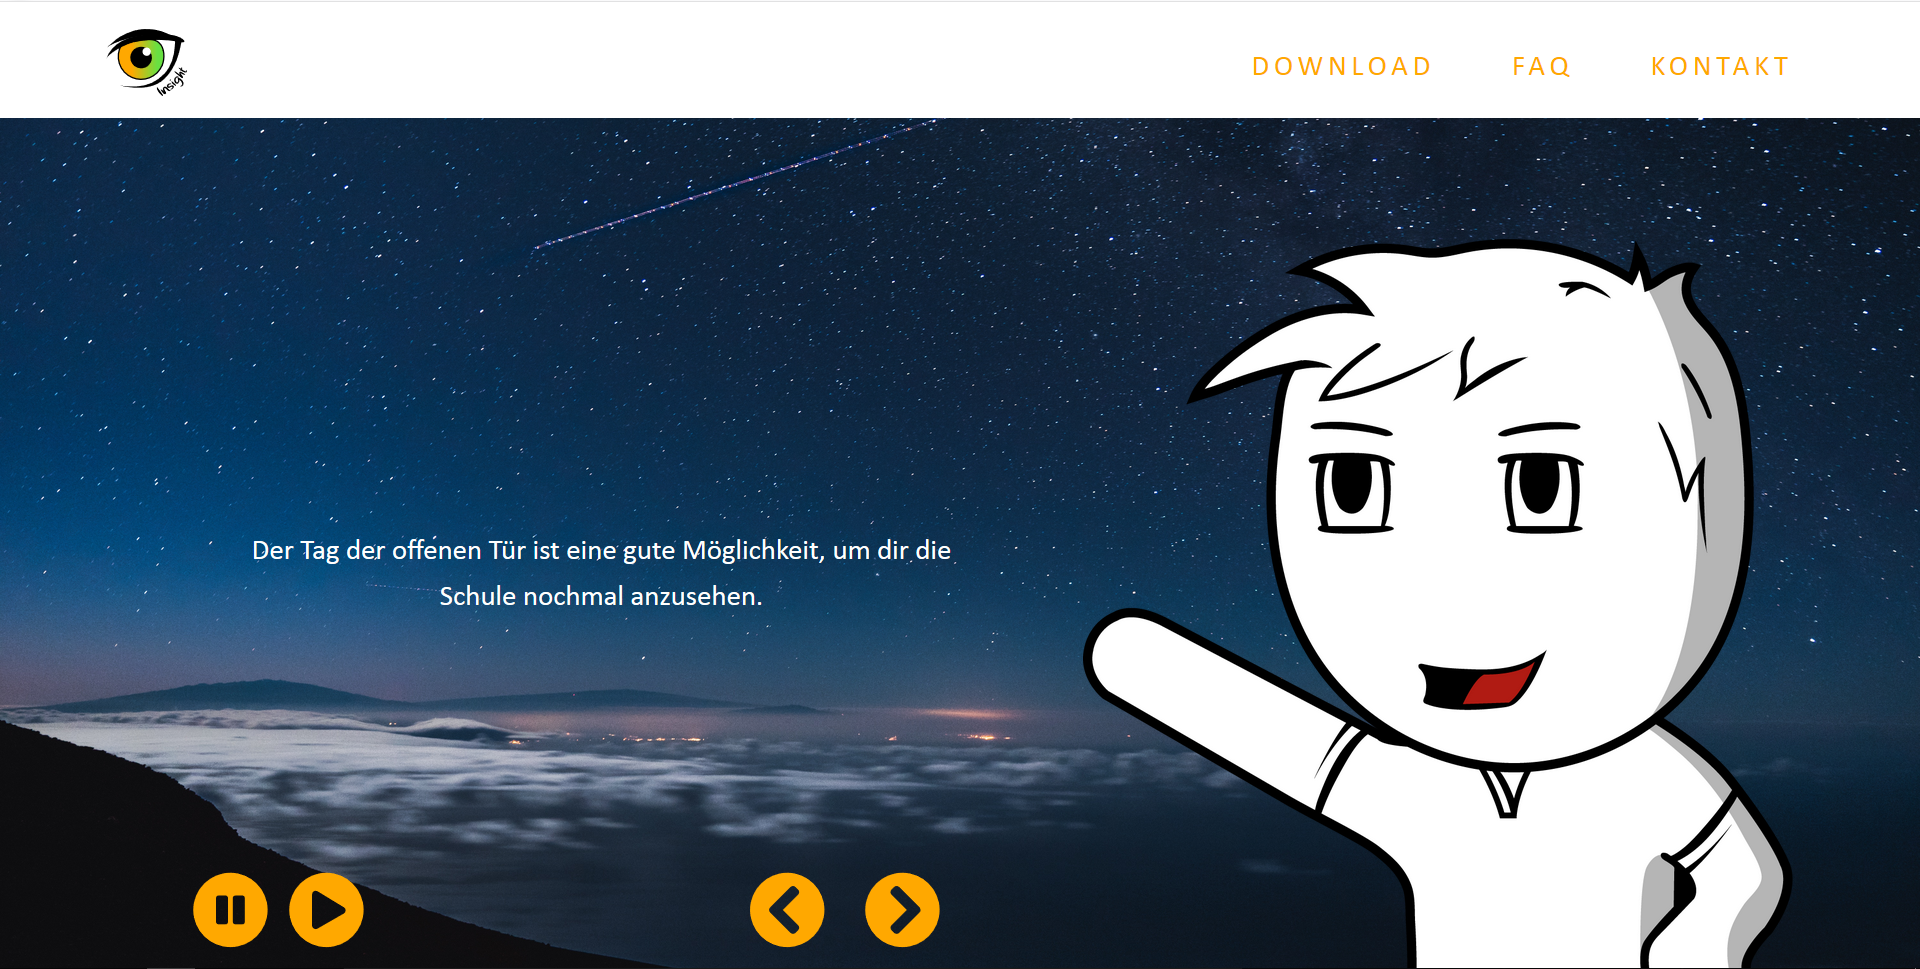
\includegraphics[width=12cm,height=12cm,keepaspectratio]{webseite_abb20} 
	\caption{Der Tag der offenen Tür}
\end{figure}
\paragraph{Lektion 10} \leavevmode \\
In der zehnten Lektion verabschiedet sich Rene Weg vom User. Doch bevor die Reise zu Ende ist, gibt es noch ein Bonus-Video. Die Intention dieses Videos ist zu zeigen, was ein Absolvent der HTL Rennweg beherrscht und was ein Schüler der zweiten Klasse, alles in so kurzer Zeit gelernt hat. Durch den Kontrast zwischen dem Absolventen und dem Schüler, soll klargemacht werden, dass wenn man in die Medientechnik geht andere Interessen hat und das nicht jeder Schüler gleich ist. \leavevmode \\
In dem folgenden Absatz werden die technischen Aspekte der interaktiven Elemente erläutert.
\begin{figure} [h]
	\centering
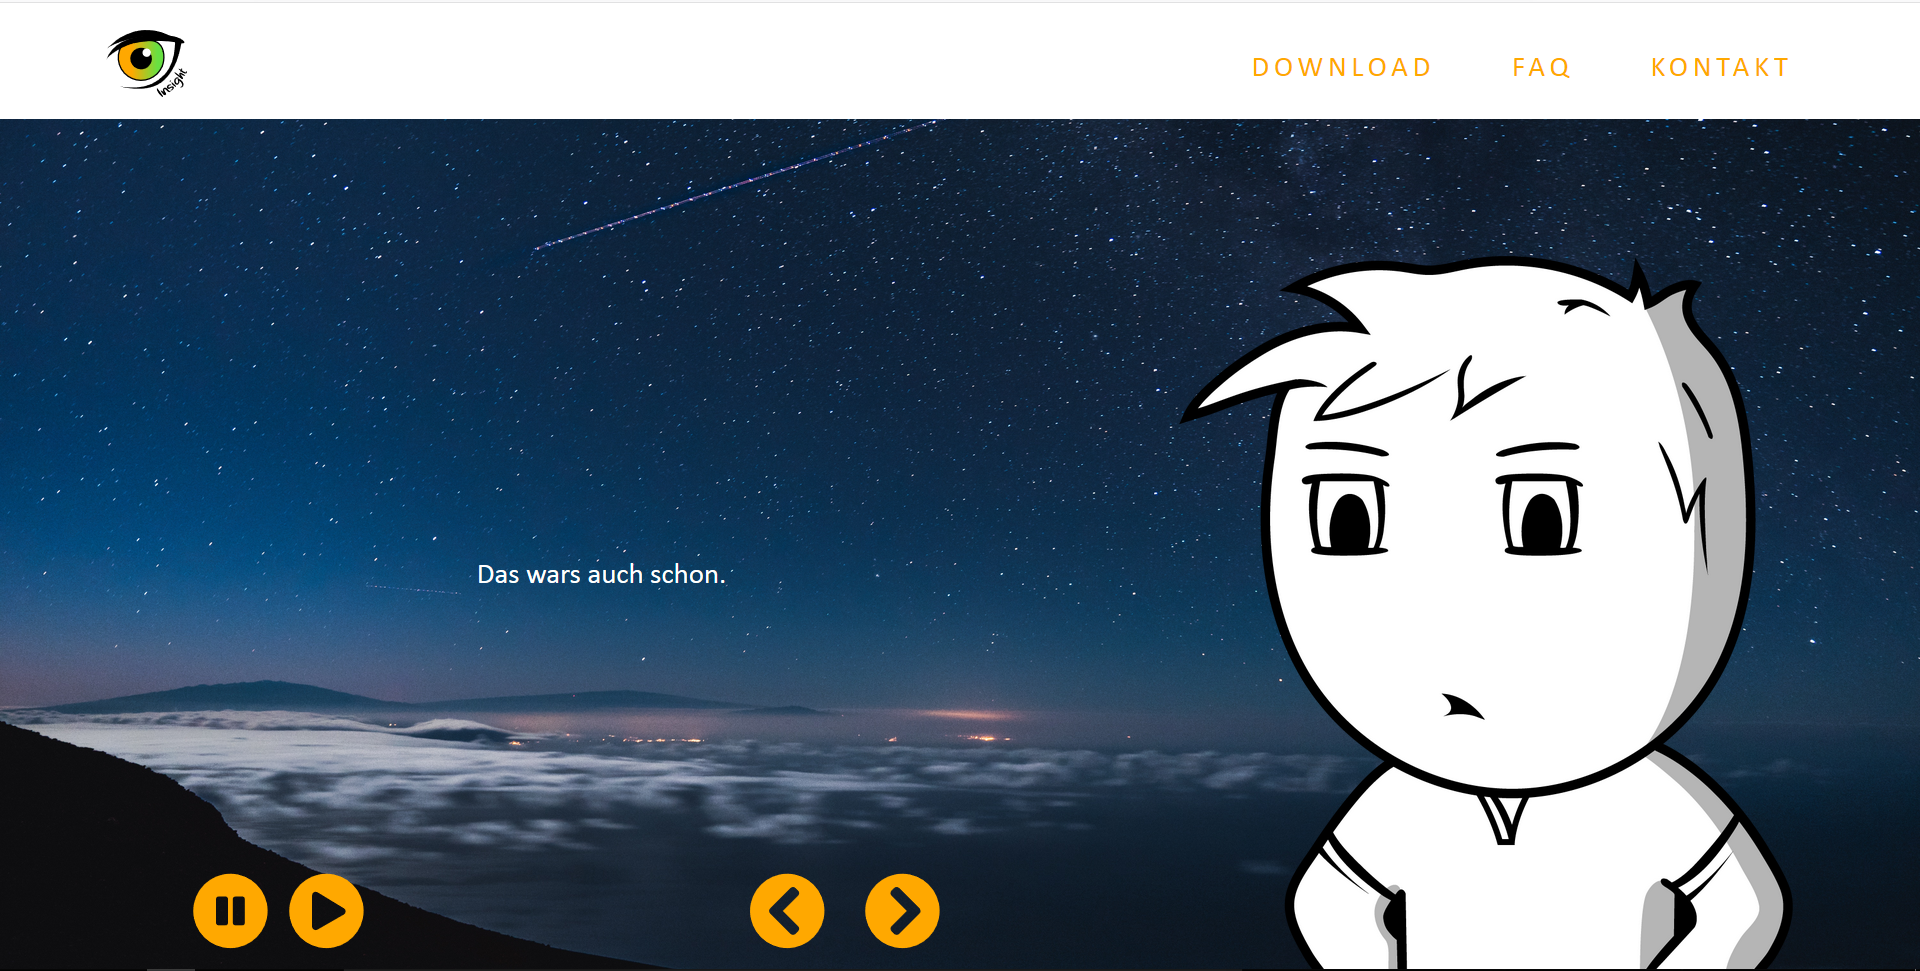
\includegraphics[width=12cm,height=12cm,keepaspectratio]{webseite_abb21} 
	\caption{Das Ende}
\end{figure}
\subsection{Interaktive Elemente}
Storytelling funktioniert nicht ohne Interaktivität.  Dafür entwickelte das Team vier interaktive Elemente, welche einen Einblick in die Medientechnik geben. 
\subsubsection{Timeline}
Um den Usern zu zeigen, wie wichtig es ist Inhalte so spannend wie möglich zu machen, wurde eine Timeline erstellt. Diese wurde mithilfe von timeline.js erstellt, welche mittels einer Excel-Tabelle eine Timeline generiert, welche anschließend angepasst werden kann. Somit ist keine Programmierarbeit nötig und es wird gezeigt, dass man nicht unbedingt programmieren muss, um spannenden Inhalt zu erstellen.
\begin{figure} [h]
	\centering
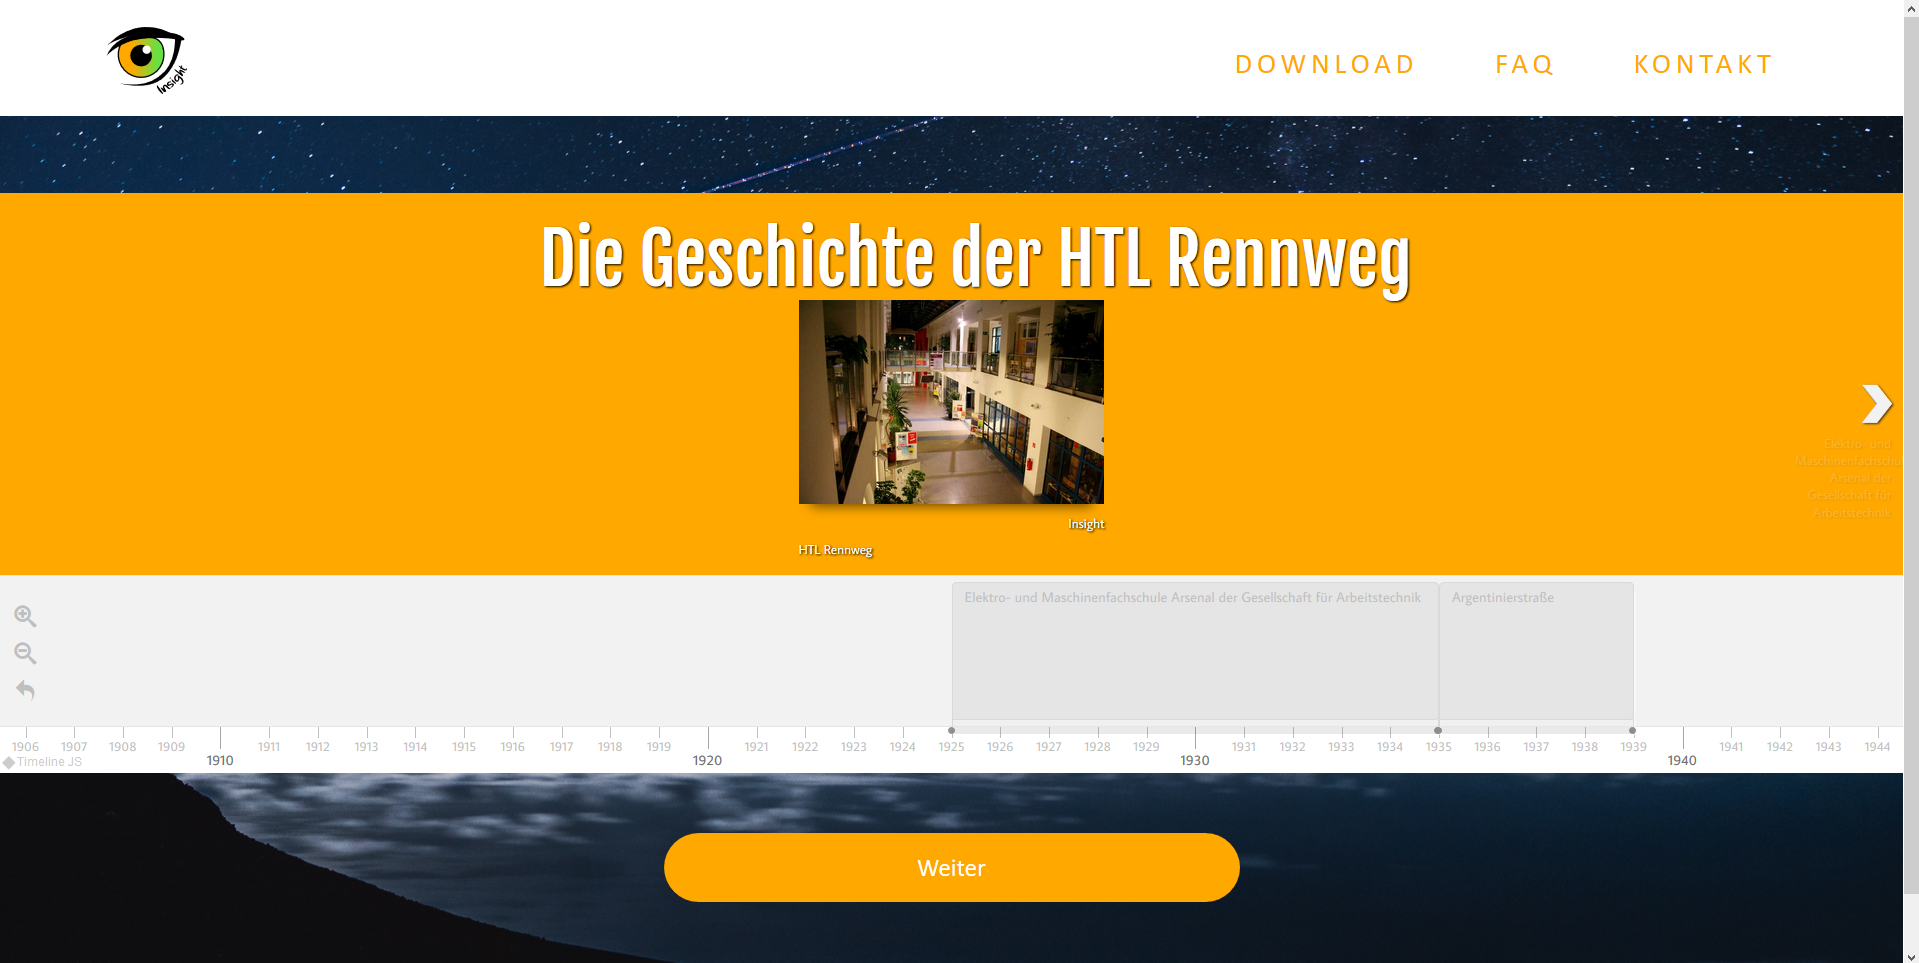
\includegraphics[width=12cm,height=12cm,keepaspectratio]{webseite_timeline} 
	\caption{Die Timeline}
\end{figure}
\subsubsection{Memory}
Das Memory-Spiel kommt in der fünften Lektion vor. Dieses ist ein sehr populäres Spiel, welches jeder kennt. Das Memory-Spiel wurde mit Hilfe eines Tutorials programmiert. Die Webseite scotch.io \cite{memorytutorial} hat ein funktionales Memory Spiel programmiert, welches nachgebaut wurde. Allerdings wurden die Elemente nicht eins zu eins übernommen, sondern auf die Wünsche des Teams angepasst. Zuerst wurde eine Infrastruktur aufgebaut. 
\begin{figure} [h]
	\centering
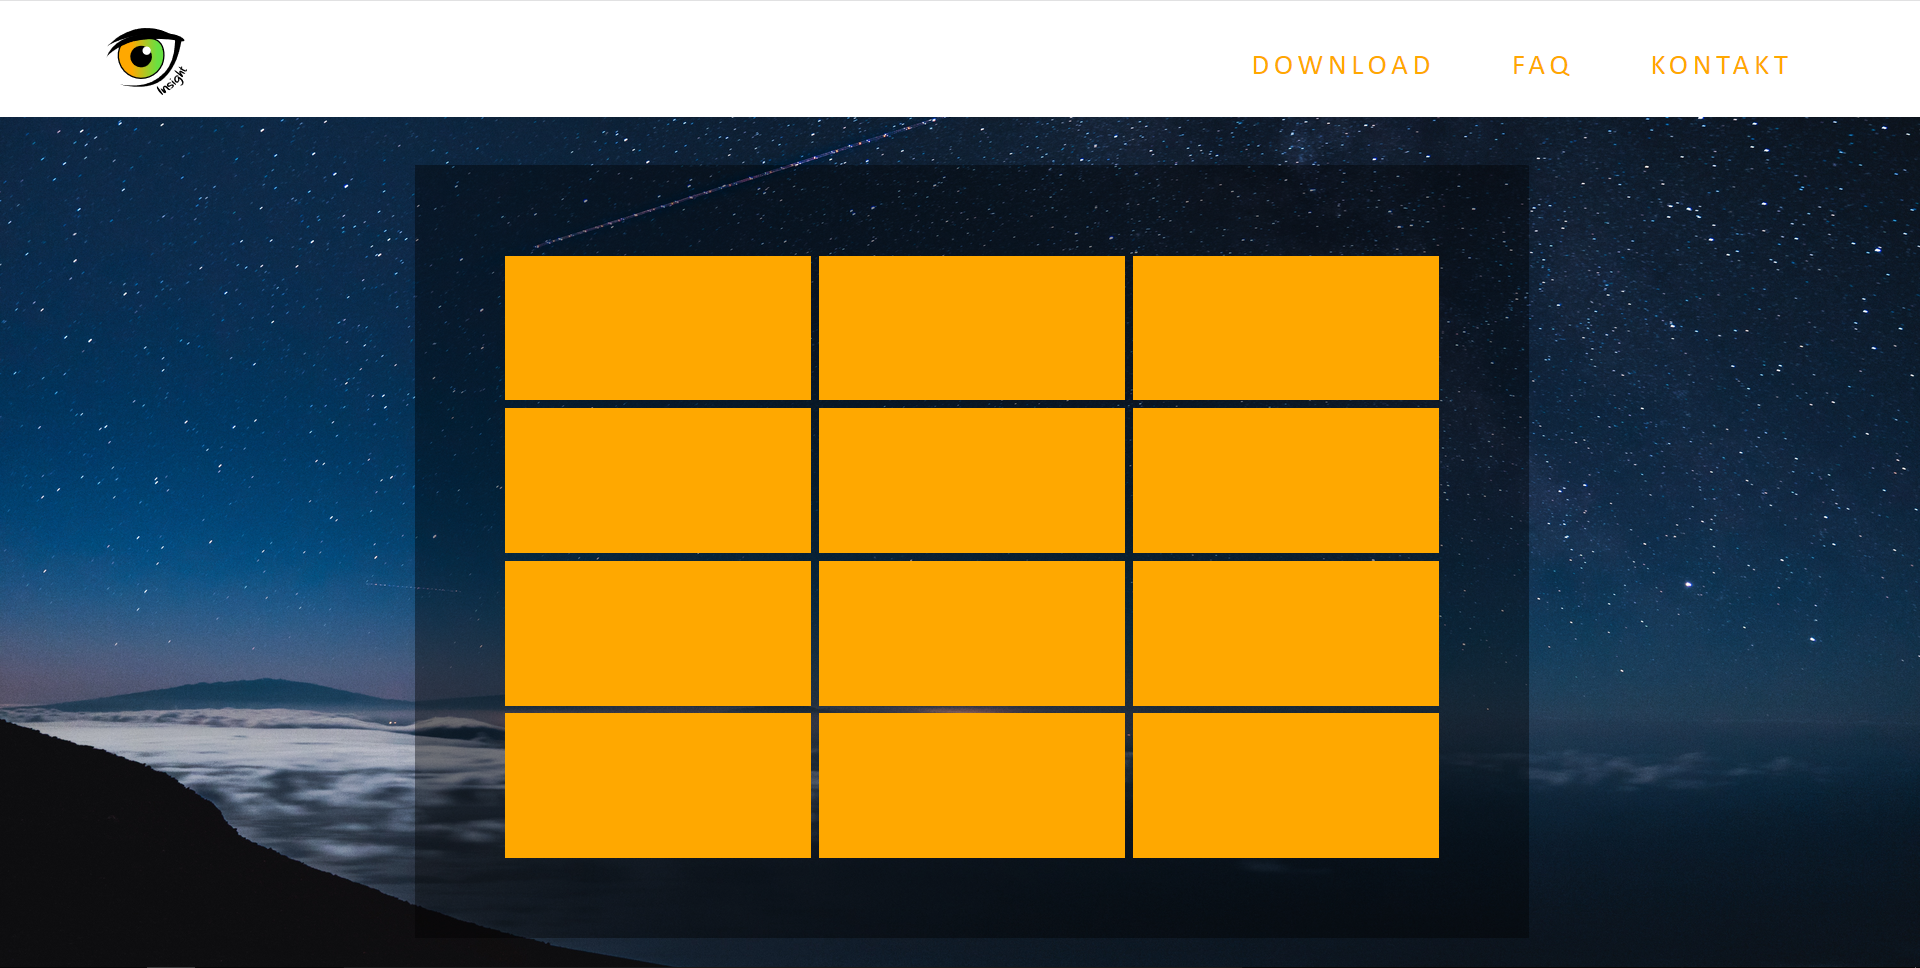
\includegraphics[width=12cm,height=12cm,keepaspectratio]{webseite_memory} 
	\caption{Die Infrastruktur des Memory Spieles}
\end{figure}
Dabei wurden immer zwei Elemente erstellt, welches dieselben Icons haben. Im JavaScript Code werden die Karten geladen und zwischen drei Klassen getoggelt. Die Klasse „open“ öffnet die Karte, „show“ sorgt dafür, dass die Karte geöffnet bleibt und „disable“ sorgt dafür, dass die Karte gesperrt ist. Danach wurde eine Klasse geschrieben, welche die Karten mischt. Sobald das HTML-Dokument aufgerufen wird, wird das Spiel geladen. Natürlich musste auch eine Klasse geschrieben werden, welche überprüft, ob die Karten identisch sind. Danach bleiben die Karten offen. Wenn sie nicht identisch sind, drehen sich die Karten wieder um. 
\begin{figure} [h]
	\centering
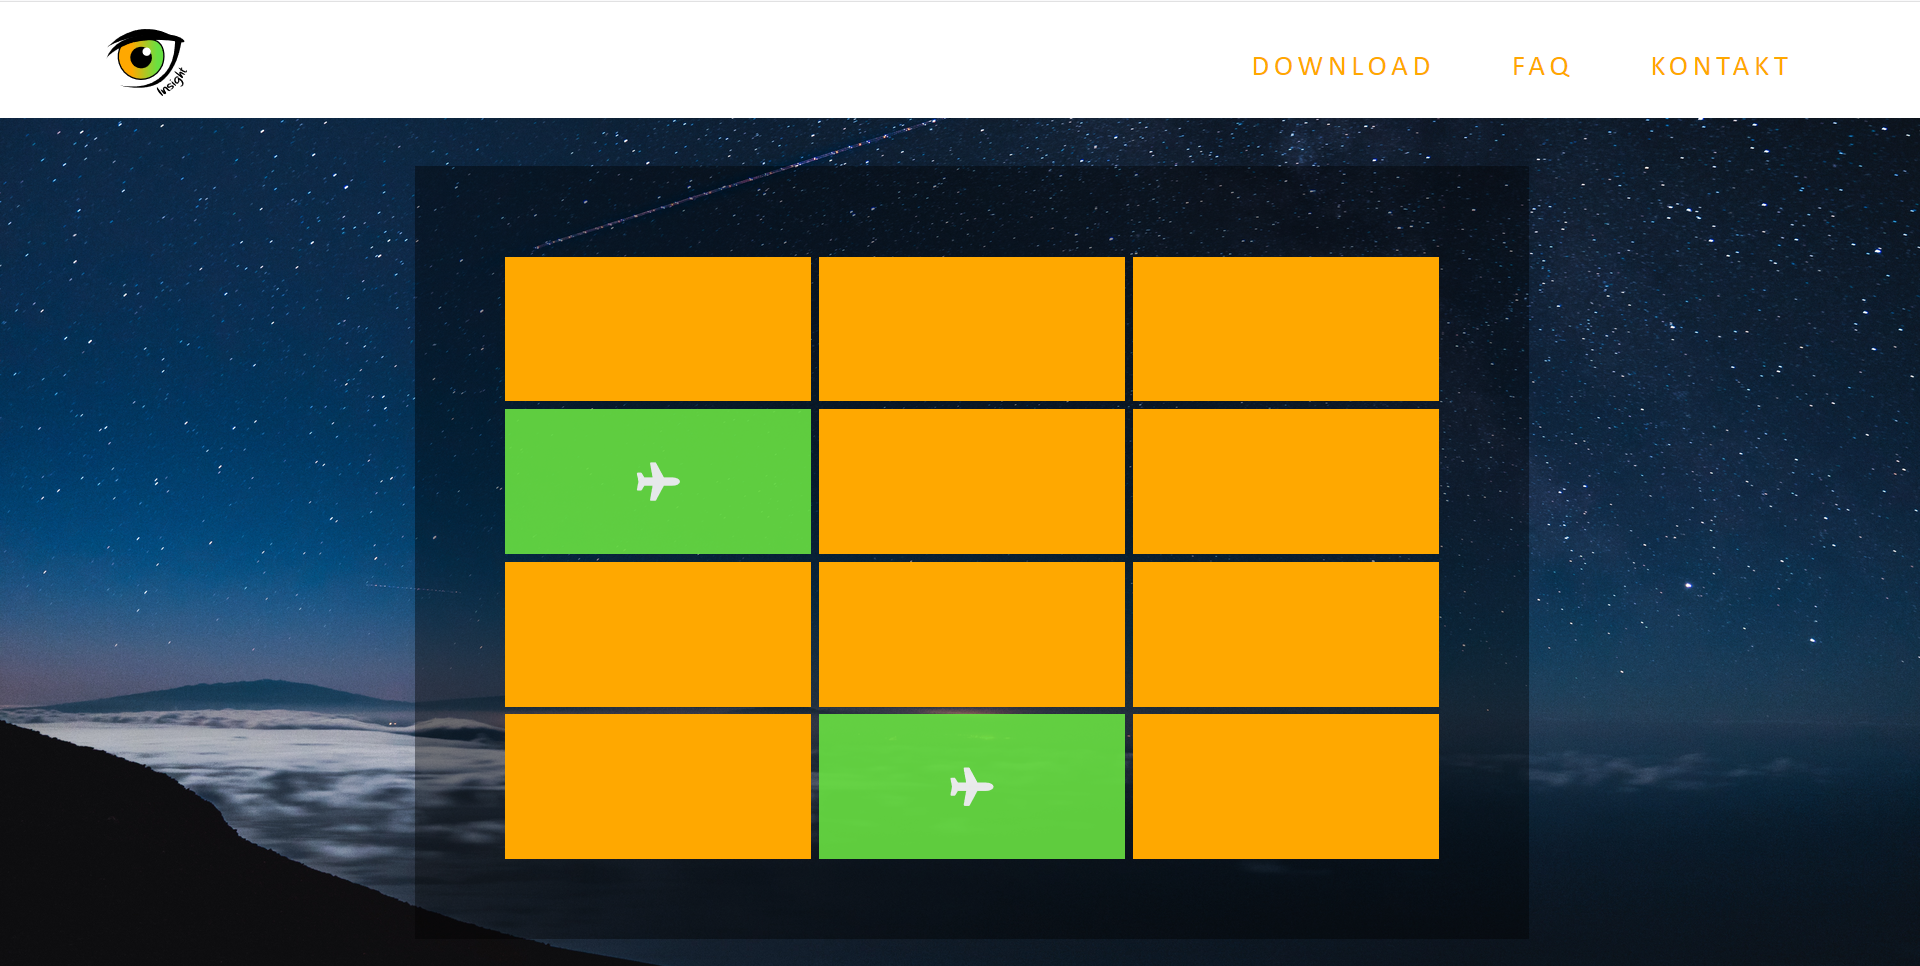
\includegraphics[width=12cm,height=12cm,keepaspectratio]{webseite_memory_1} 
	\caption{Die Karten bleiben offen, wenn sie identisch sind}
\end{figure}
Nachdem alle Karten geöffnet wurden, wird der User dazu aufgefordert auf einen Button zu drücken, welcher ihn zur nächsten Lektion bringt. 
\begin{figure} [h]
	\centering
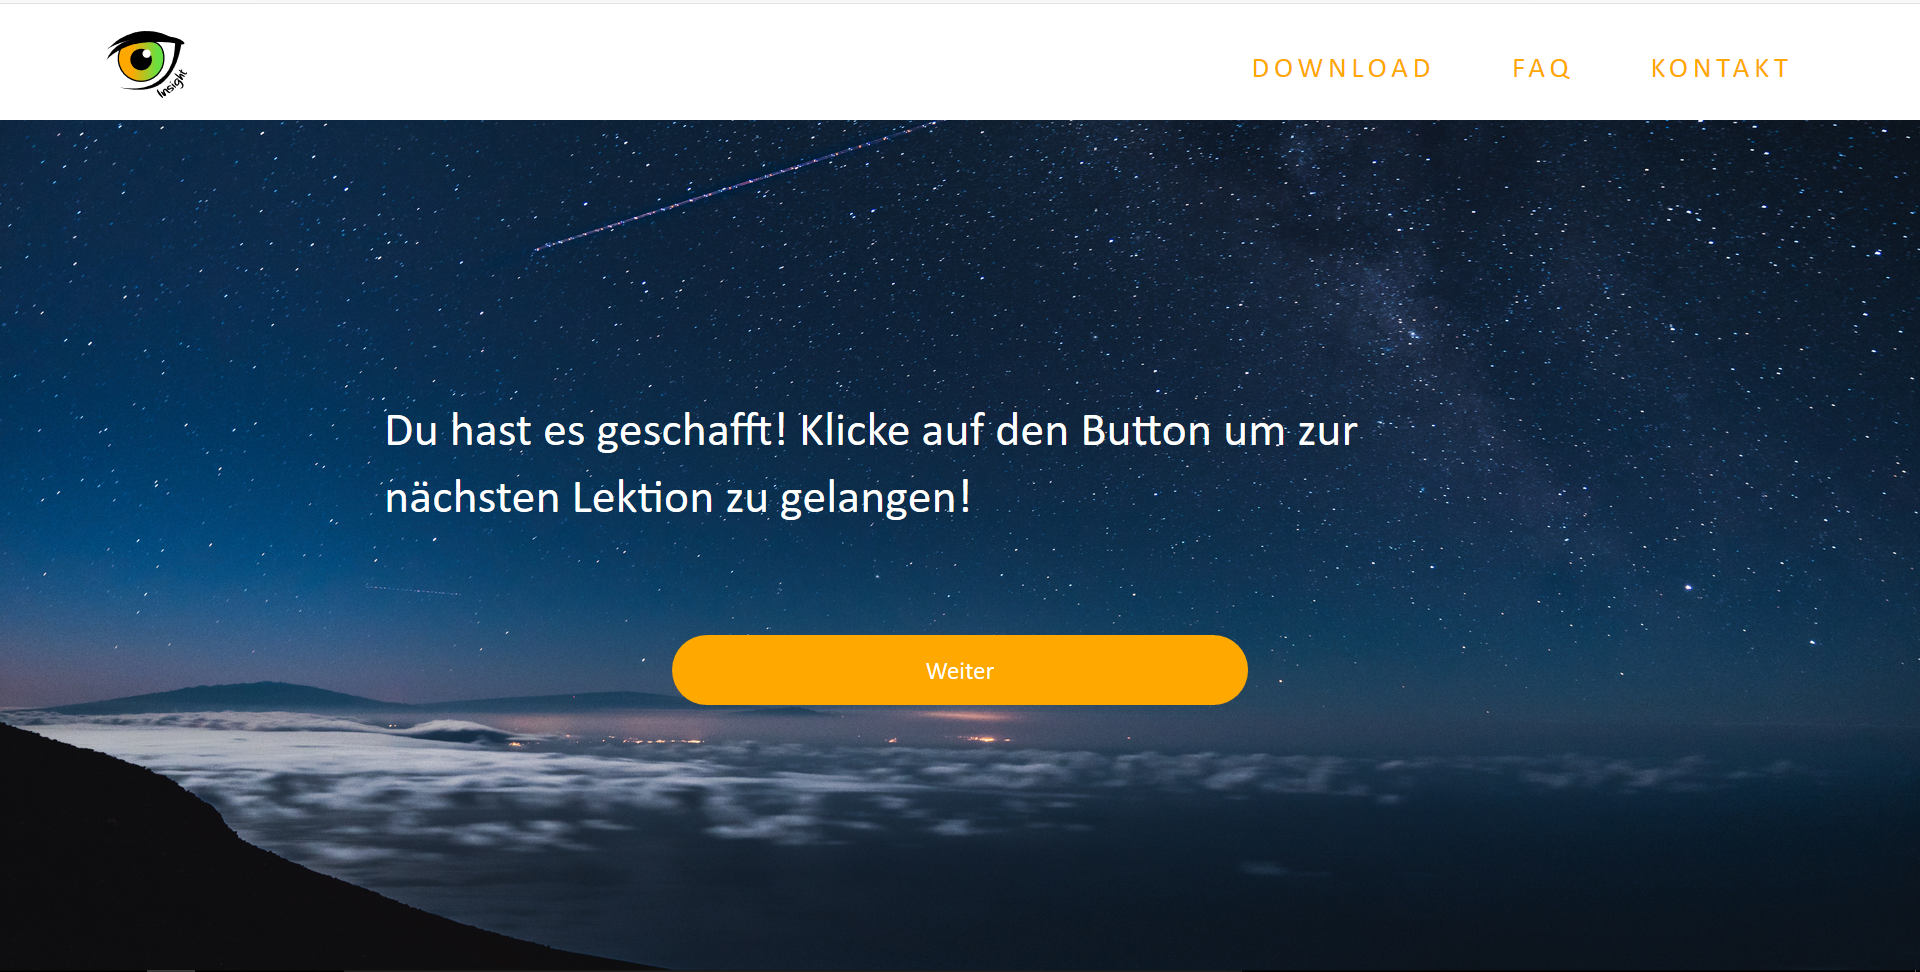
\includegraphics[width=12cm,height=12cm,keepaspectratio]{webseite_memory_2} 
	\caption{Am Ende des Spieles}
\end{figure}
\subsubsection{Animationen}
In der sechsten Lektion geht es um Animationen. Dabei hat sich das Team überlegt, einen Spielplatz für User zu kreieren, wo sie Planeten verschieben können. Außerdem gibt es eine Rakete, welche ebenfalls verschoben werden kann. Dies wurde mit dem JavaScript Modul interact.js erstellt. Der Source-Code wurde aus dem Tutorial, der Seite von interact.js entnommen und geändert. 
\begin{figure} [h]
	\centering
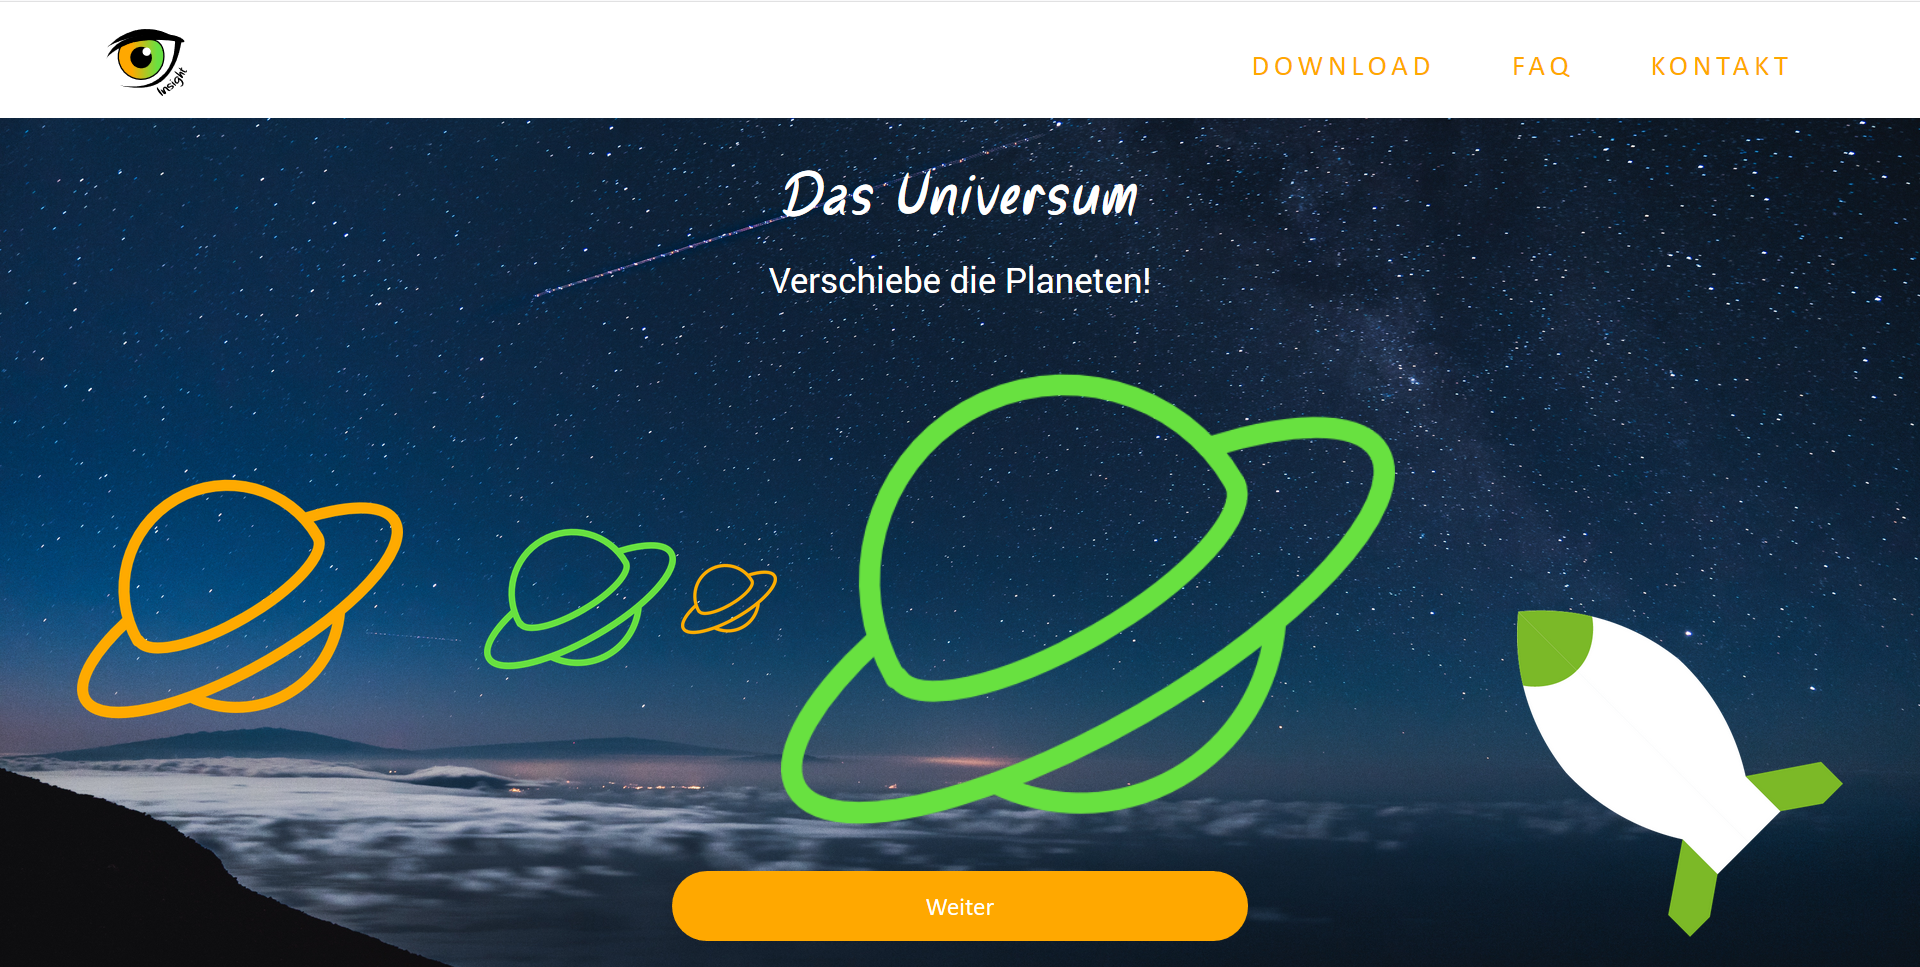
\includegraphics[width=12cm,height=12cm,keepaspectratio]{webseite_universum} 
	\caption{Der User kann ein Universum kreieren}
\end{figure}
\subsubsection{Schrödingers Katze}
In der siebten Lektion geht es um Schrödingers Katze. Die Idee war es ein Bild von einer Kiste auf die Webseite zu platzieren. Wenn der User über die Kiste fährt, sollte eine Katze in der Kiste erscheinen. Dies wurde mit Hilfe von EaselJS programmiert. Dabei wurde ein Bild von einer leeren Kiste und von einer Kiste mit einer weißen Katze übereinandergelegt. Wenn der User über die leere Kiste fährt, wird das Bild subtrahiert und das Bild mit der weißen Katze kommt zum Vorschein. Damit wird eine Anspielung auf das Paradox gemacht. 
\begin{figure} [h]
	\centering
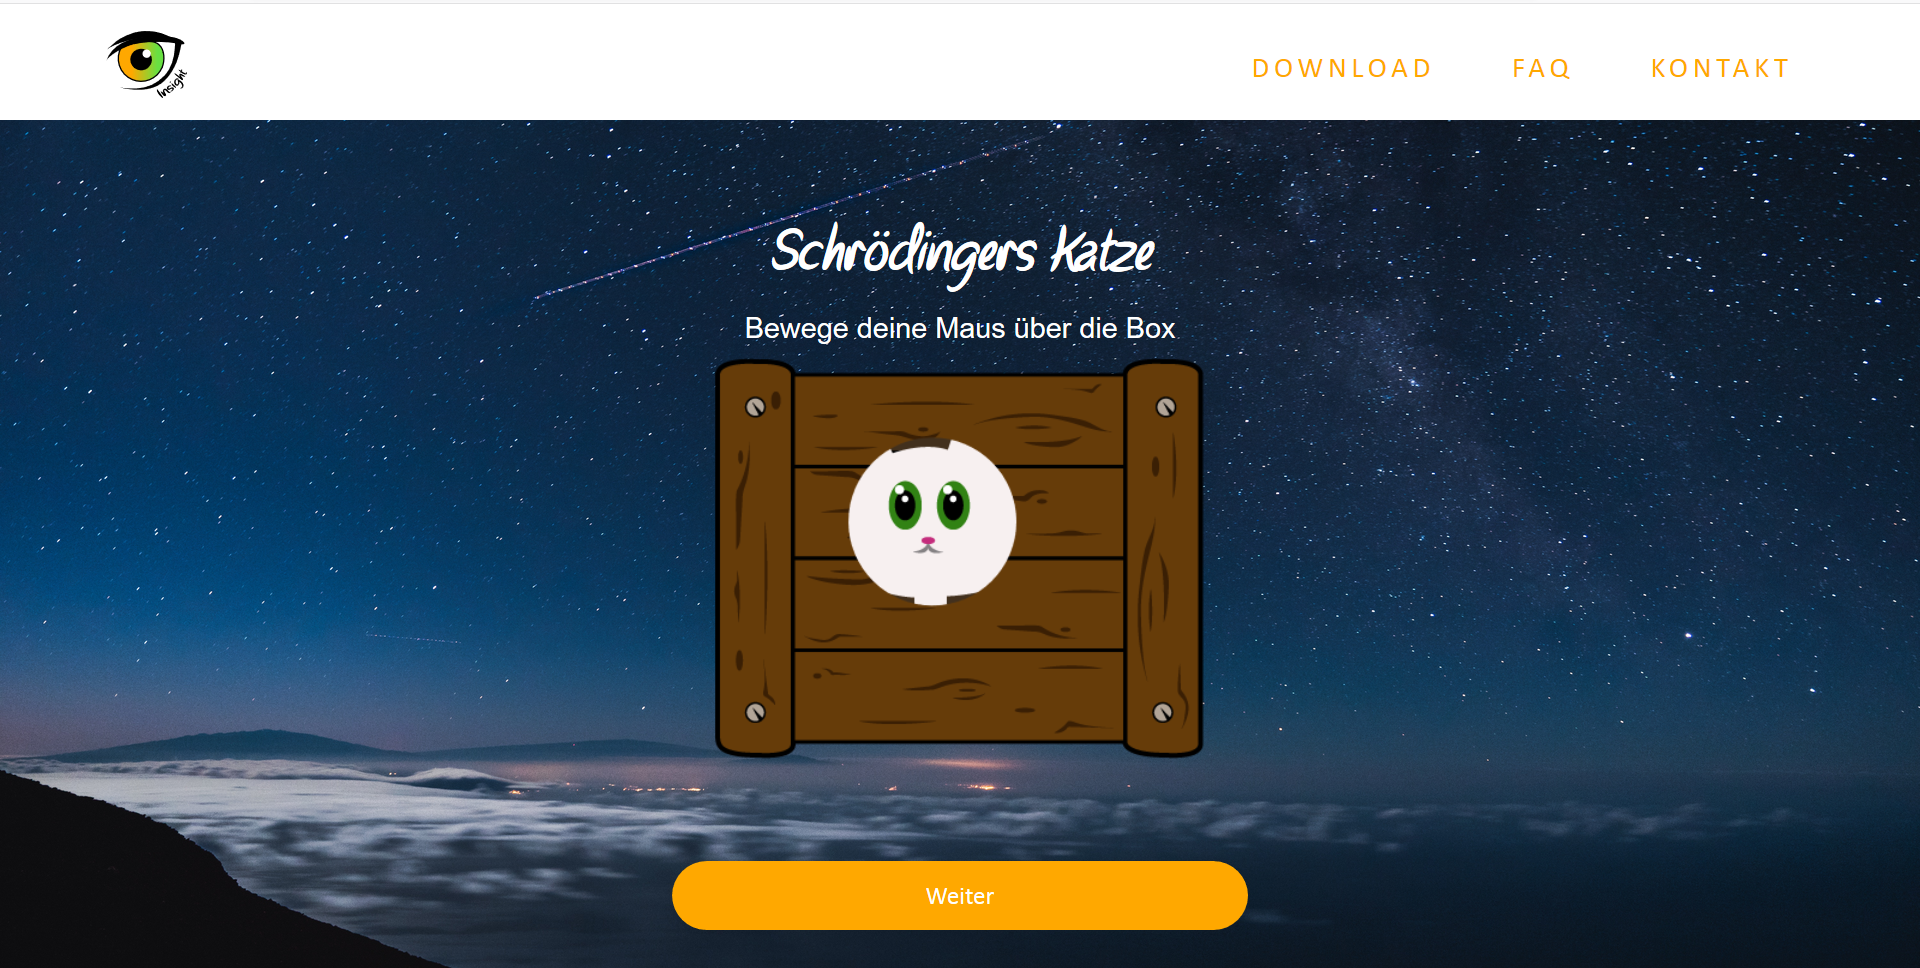
\includegraphics[width=12cm,height=12cm,keepaspectratio]{webseite_katze} 
	\caption{Schrödingers Katze}
\end{figure}


\chapter{Video}
\renewcommand{\kapitelautor}{Autor: Kerstin Schön}
\section{Interview mit dem Abteilungsvorstand}
\subsection{Idee}
Die Intention des Interviews mit dem Abteilungsvorstand, Dr. Hager, war es, Interessenten allgemeine Informationen über die Schule näher zu bringen. Das Ziel war es, die wichtigsten Informationen kurz und prägnant rüberzubringen, sodass der Interessent die wichtigsten Informationen, ohne lang danach zu suchen, erhält.
\begin{figure}[H]
	\centering	
	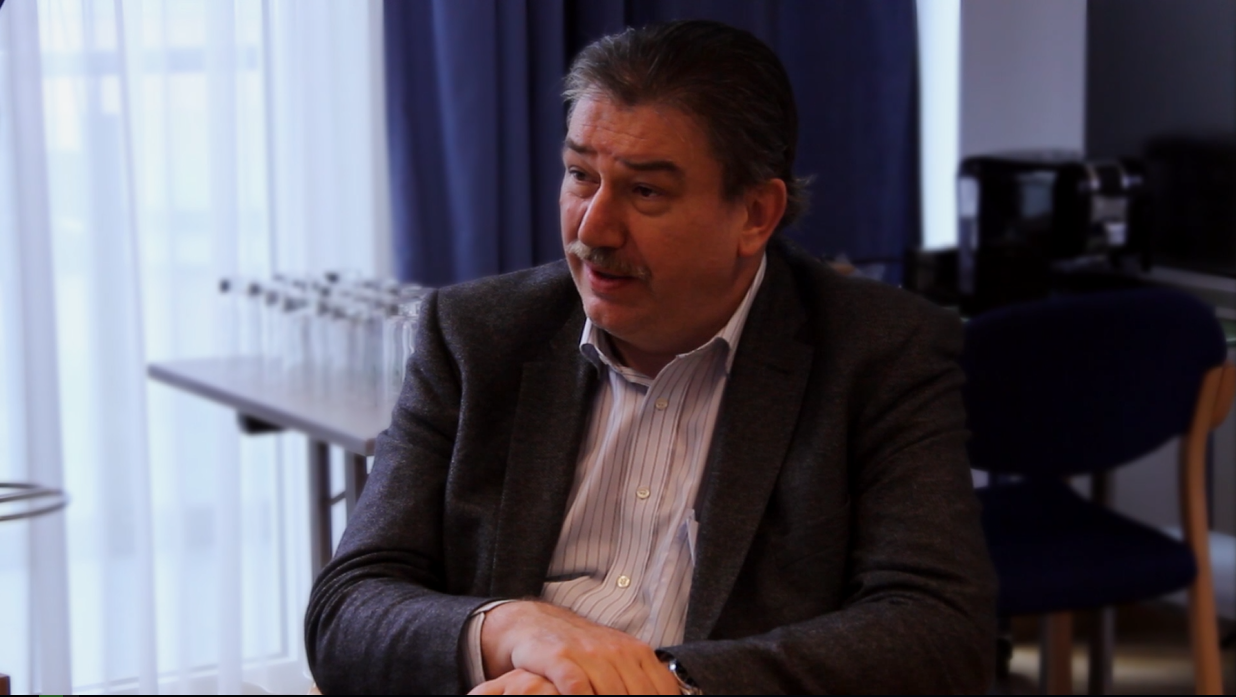
\includegraphics[width=0.8\textwidth]{abb23} 
	\caption{Interview mit dem Abteilungsvorstand}
\end{figure}
\section{Tag der offenen Tür}
\subsection{Idee}
Das Tag der offenen Tür Video dreht sich um die Interessenten, die sich die Schule am Tag der offenen Tür angeschaut haben. Hierbei wurden Fragen, wie: "Wie ist dein erster Eindruck von der Schule?", oder "Kannst du dir vorstellen dich hier anzumelden?" gestellt. Weiters spricht am Ende des Videos ein Lehrer über die Schule und erklärt den Unterschied zwischen einer HTL und einer AHS.
\begin{figure}[H]
	\centering	
	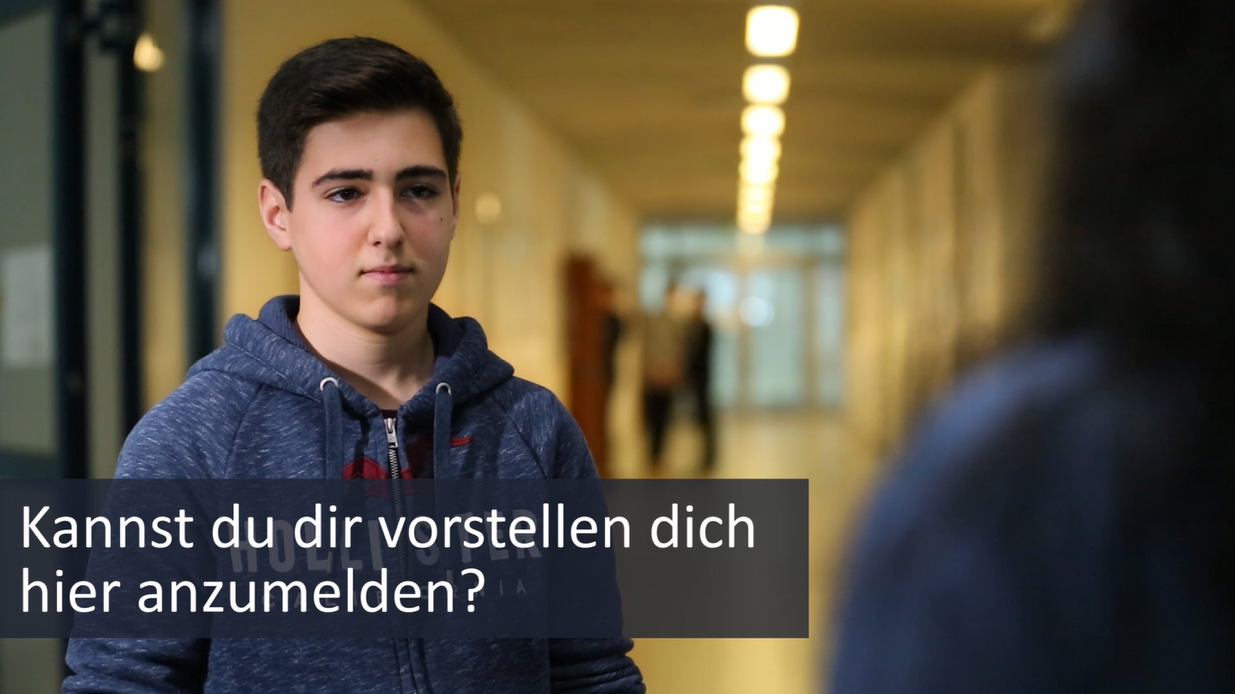
\includegraphics[width=0.8\textwidth]{abb24} 
	\caption{Tag der offenen Tür}
\end{figure}
\section{Video mit einem Absolvent}
\subsection{Idee}
In dem Video, beziehungsweise dem Quiz, mit dem Absolventen und dem Schüler der zweiten Klasse geht es darum, dass dem Absolventen und dem Schüler Fragen gestellt werden, wobei sie 45 Sekunden Zeit haben diese zu beantworten. Derjenige, der die Frage falsch beantwortet, muss ein Jelly-Bean essen, wobei man nicht weiß, ob es ein gutes oder ein schlechtes ist. Die Intention dieses Videos ist es zu zeigen, dass die Medientechnik ein enorm großer Bereich ist, bei dem man nicht alles erlernen kann. So spezialisiert sich jeder Schüler meist auf ein Gebiet, das er dann auch dementsprechend gut kann. Was jedoch zu beachten ist, ist, dass die Schüler dennoch die Grundlagen der anderen Medientechnik Themen lernen und auch können.
\begin{figure}[H]
	\centering	
	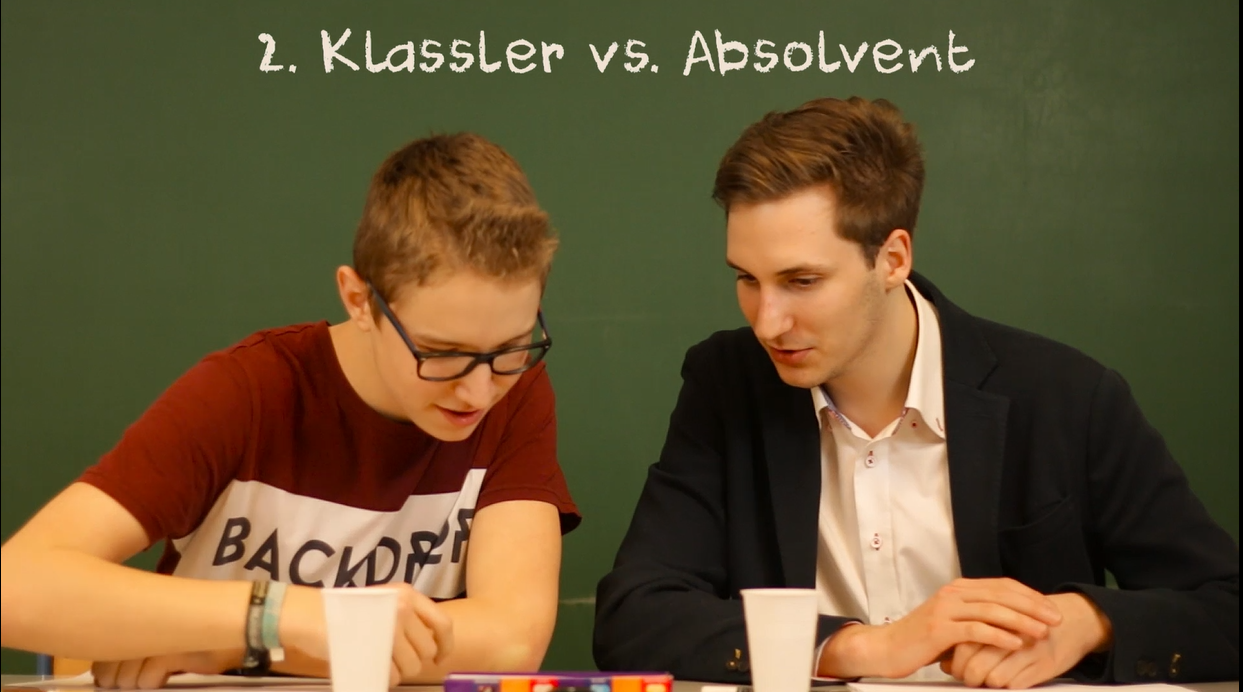
\includegraphics[width=0.8\textwidth]{abb25} 
	\caption{Video mit einem Absolvent}
\end{figure}
\section{Technik}
\subsection{Auflösung}
Bei der Auflösung wird heutzutage unter SD, HD (2k), Digital Cinema (2k) und UHD (4k/8k) unterschieden. SD bedeutet Standard Definition und dominierte früher das Fernsehen. Heutzutage ist der Standard nicht mehr Standard-Definiton, sondern High-Definition. Obwohl bei Smartphones, TV-Geräten und Kameras schon Full-HD, also 1920 x 1080 px, der Vorreiter ist, wird zumindest im deutschen Fernsehen noch im normalen HD Format, also 1280 x 720 px, ausgestrahlt.\citep{joerg}\newline
Bei den Videoaufnahmen wurde immer im Full-HD Format aufgenommen, also mit 1920 x 1080 px, da heutzutage die meisten Videos, von den Jugendlichen, am Smartphone angesehen werden.
\subsection{Aspect-Ratio - Seitenverhältnis}
Früher, als SD das Standard-Fernsehformat war, war das Seitenverhältnis eines Fernsehbildes 4:3. Jedoch wurde später aus 4:3, 16:9, was auch heute im HD Format noch beibehalten wurde. Das SD Format verwendet rechteckige Pixel, was die Folge hat, dass ein SD Bild immer die gleiche Anzahl von Pixeln hat, nämlich 720 x 576. \textit{"Nur werden einmal rechteckige Pixel mit einem Seitenverhältnis von 1,46:1 (= 16:9) und einmal von 1,09:1 (= 4:3) verwendet."}(Jörg Jovy, 2017, S.108)\newline 
Man nennt dies auch anamorph. "Anamorph bedeutet, dass die Pixel des Films nicht quadratisch sind, sondern rechteckig." (Jörg Jovy, 2017, S.572)\newline
Da Computer und HD-Bilder nur quadratische Pixel anzeigen, aber ein SD Fernsehformat rechteckige, muss man bei der Auswahl des Formats berücksichtigen, wo man das Video oder den Film schlussendlich abspielen möchte.\citep{aspect}
\subsection{Bildrate}
Seit 1967 wird im deutschen Fernsehen mit dem sogenannten PAL Format (=Phase Alternative Line) gesendet. Im PAL Format werden 25 Bilder pro Sekunde oder 50 Halbbilder pro Sekunde gesendet. Jedoch herrscht in den USA nicht das PAL Format, sondern das sogenannte NTSC Format (=National Television Systems Committee), welches 30 Vollbilder pro Sekunde oder 60 Halbbilder pro Sekunde sendet. Diese unterschiedlichen Bildraten sind der Tatsache geschuldet, da in Europa eine Wechselspannungsfrequenz von 50Hz herrscht, und in den USA eine von 60Hz.\citep{bildrate}\newline
Bei Videoaufnahmen wurde mit 25fps (= frames per second), also mit 25 Vollbildern in der Sekunde, aufgenommen.
\subsection{Farbraum}
Rot, Grün und Blau sind die drei Grundfarben des RGB Farbraums. Aus den drei Grundfarben bilden sich alle anderen Farben, die im RGB Farbraum möglich sind, was man RGB-Farbmischung nennt.\begin{quote}"Bei einer 8-Bit-Codierung pro Farbe stehen 256 verschiedene Farbwerte zur Verfügung. Aus der Mischung ergeben sich theoretisch 16,78 Mio. verschiedene Farbwerte (= 256 x 256 x 256)." (Jörg Jovy, 2017, S. 113)\end{quote} Schwarz enthält keine Farbinformation von den drei Grundfarben, wohingegen Weiß die Mischung aller drei Grundfarben ist. Der Farbraum des HD Standards ist RGB oder auch genannt als sRGB. Bei der Kamera kann zwischen sRGB und Adobe RGB umgestellt werden. Meist wird der Adobe RGB Farbraum verwendet, da er einen größeren Farbraum bietet. Wie man anhand der Abbildung \ref{fig:abb16} sehen kann, hat der Adobe RGB Farbraum mehr Grüntöne als der sRGB Farbraum.\citep{farbraum}
\begin{figure}[H]
\centering
	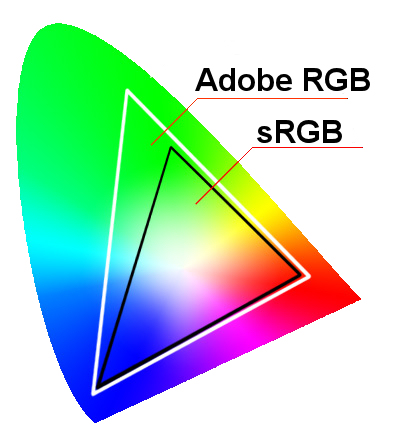
\includegraphics[width=0.3\textwidth]{abb16}
	\caption[sRBG und Abobe RGB Farbraum]{sRBG und Abobe RGB Farbraum\footnotemark}\label{fig:abb16}
\end{figure}
\footnotetext{Quelle: https://photo.stackexchange.com/questions/86340/adobe-rgb-monitor-outside-photoshop}
\subsection{Farbabtastung}
Bei der Farbunterabtastung handelt es sich um eine Komprimierung von  der Übertragung der Signale. Da ein unkomprimiertes Signal eine zu große Bandbreite in Anspruch nehmen würde, muss das Signal komprimiert werden. Dafür wird die Farbabtastung in Betracht gezogen. Da das menschliche Auge die Helligkeitskontraste besser auflöst als die Farbkontraste, wird bei der Farbabtastung die Helligkeit, oder Luminanz, mit der vollen Datenbreite zur Verfügung gestellt. Die Farbinformation wird, bei der Farbabtastung, jedoch reduziert. Daraus ergibt sich dann ein voll aufgelöstes Signal mit der Farbabtastung von 4:4:4. Ein bereits komprimiertes Signal hat eine Farbunterabtastung von 4:2:2, 4:2:0 oder von 4:1:1.\citep{farbabtastung}
\paragraph{4:2:2}
\leavevmode \\
Bei der Farbunterabtastung von 4:2:2 wird bei jedem Pixel der Helligkeitswert abgetastet, wobei der Farbwert nur bei jedem zweiten Pixel abgetastet wird.\citep{farbabtastungZwei}
\paragraph{4:2:0}
\leavevmode \\
\begin{quote}"Beim Subsampling von 4:2:0, erfolgt die Abtastung der Chrominanzsignale für jeweils vier quadratisch angeordnete nebeneinander liegende Pixel. Wie bei den anderen Subsampling-Verfahren auch, wird das Luminanzsignal bei jedem Pixel abgetastet." (https://www.itwissen.info/Farb-Subsampling-color-subsampling.html [Zugriff: 18.03.2018])\end{quote}
\paragraph{4:1:1}
\leavevmode \\
Bei der Farbunterabtastung von 4:1:1 werden die Chrominanzsignale bei jeder vierter Abtastung des Helligkeitssignal abgetastet.\citep{farbabtastungZwei}
\begin{figure}[H]
	\centering	
	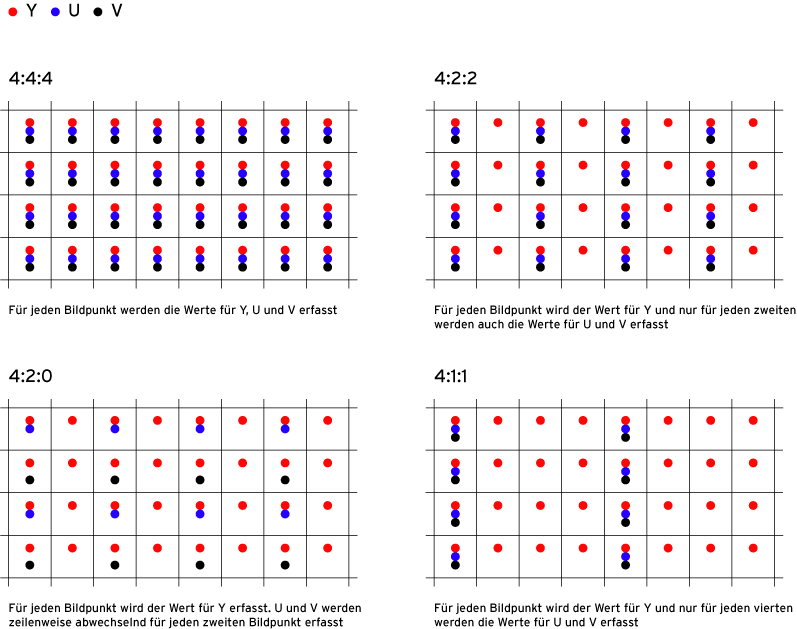
\includegraphics[width=0.8\textwidth]{abb15} 
	\caption[Farbabtastung]{Farbabtastung\footnotemark}
\end{figure}
\footnotetext{Quelle: http://www.dma.ufg.ac.at/app/link/Grundlagen\%3AVideo.Postproduction/module/3927}
\subsection{Weißabgleich}
Bevor man ein Bild schießt, oder ein Video dreht, führt man zuerst einen Weißabgleich durch. Dabei wird zwischen manuellen und automatischen Weißabgleich unterschieden. Hierbei wird die Lichtfarbe beziehungsweise die Farbtemperatur gemessen und der Weißabgleich darauf eingestellt. Die Farbtemperatur wird in Kelvin angegeben. Eine Kerze hat eine sehr rötliche und warme Farbstimmung mit einer Farbtemperatur von 1.500 Kelvin, wohingegen das Tageslicht neutral wirkt und eine Farbtemperatur von 5.000 bis 6.000 besitzt. Um den Weißabgleich manuell abzustimmen, wird ein weißes Blatt Papier vor die Kamera gehalten, und der Weißabgleich kann somit eingestellt werden. Das weiße Blatt Papier ist jedoch nur ein Hilfsmittel. Optimal wäre, eine professionelle Graukarte zu verwenden. Das Problem mit dem Papier ist, dass es optische Aufheller, die den Blauanteil erhöhen, besitzt. Das heißt, da die Kamera den zu hohen Blauanteil korrigiert, wird das Bild schlussendlich leicht gelbstichig.\citep{weissabgleich}

\section{Kameramodelle}
\subsection{DSLR Kamera - Aufbau}
DSLR bedeutet Digital Single Lens Reflex und sind Spiegelreflexkameras mit digitalem Aufnahmesensor. Beispiele für eine Spiegelreflexkamera sind die Canon EOS 60D oder die Canon EOS 70D. In der folgenden Abbildung wird der Aufbau einer DSLR Kamera erklärt.\newline 
Wie man in der Abbildung \ref{fig:abb13} sehen kann, geht das Licht zuerst durch die Linse des Objektivs (1). Anschließend trifft das Licht auf den Schwingspiegel (2), welcher das Licht auf die Mattscheibe (5) reflektiert. Daraufhin verkleinert es die Sammellinse (6) auf die Größe des Suchers. Da das Bild noch spiegelverkehrt ist, spiegelt es das Pentaprisma (7) und kann so im Sucher (8) dann angezeigt werden. Als nächstes wird der Auslöser getätigt. Durch das Klicken auf den Auslöser wird der Spiegel nach oben geklappt und der Weg zum Schlitzverschluss (3) wird freigegeben. Anschließend öffnet sich dieser Verschluss und das Licht fallt auf den Sensor (4). Zum Schluss wird das Bild abgespeichert.\citep{aufbau}
\begin{figure}[H]
	\centering
	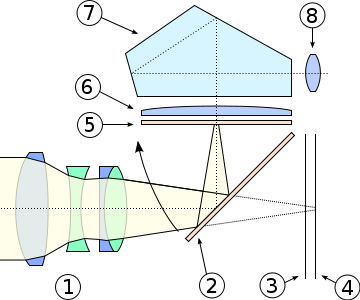
\includegraphics[width=0.6\textwidth]{abb13} 
	\caption[Aufbau einer DSLR Kamera]{Aufbau einer DSLR Kamera\footnotemark}\label{fig:abb13}
\end{figure}
\footnotetext{Quelle: http://referate.mezdata.de/sj2009/dslr\_sinan-saglam/ausarbeitung/seite2.htm}
\subsection{Sensoren}
Heutzutage gibt es zwei Vorreiter im Bereich der Sensoren. Nämlich einerseits den CMOS-Sensor und andererseits den CCD Sensor. Welcher Sensor nun auch wirklich besser ist, und in welcher Kamera welcher Sensor eingebaut werden soll, ist jedoch noch umstritten.\citep{sensor}
\paragraph{CMOS-Chips}
\leavevmode \\
Die CMOS Sensoren haben den großen Nachteil, dass das Bild bei schnellen Bewegungen, etwa wie beim Filmen von fahrenden Autos, verzerrt dargestellt wird. Dies wird auch Rolling-Shutter-Effekt genannt. Bei dem Rolling-Shutter-Effekt schauen die vertikalen Linien so aus, als würden sie umfallen, was das Bild unbrauchbar machen kann.\citep{sensor}
\paragraph{CCD-Chips}
\leavevmode \\
Die CCD Sensoren haben zwar nicht das Problem mit dem Rolling-Shutter-Effekt, jedoch sind diese Sensoren lichtempfindlicher. Das bedeutet, dass wenn das Licht direkt ins Objektiv scheint, tritt der Blooming-Effekt auf. Beim Blooming-Effekt wird das Bild von einem breiten weißen Streifen geteilt. Scheint Kunstlicht in das Objektiv, entstehen wandernde violette Streifen.\citep{ccd}
\subsection{Canon EOS 60D}
Die Canon EOS 60D DSLR (Digital Single Lens Reflex) Kamera bietet einen 18 Megapixel APS-C CMOS Sensor mit einer Größe von 22,3 mm x 14,9 mm. Die Spiegelreflexkamera nimmt mit Full HD (1920 x 1080) auf, wobei standardgemäß mit 25 Bildern pro Sekunde aufgenommen wird. Die Auflösung wird meistens mit 1080p gekennzeichnet, wobei das p für progressive steht, also für die Vollbilder.\citep{canon60}\citep{canon60Zwei}
\subsection{Canon EOS 70D}
Die Canon EOS 70D bietet einen minimal größeren Sensor im Gegensatz zu der Canon EOS 60D. Die Größe des Sensors der Canon EOS 70D beträgt 22,5 mm x 15,0 mm. Die Sensorgröße einer Kamera ist entscheidend, da folgendes gilt: "Je kleiner der Sensor, desto geringer sind die Möglichkeiten, mit einer definierten Schärfentiefe zu arbeiten." (Jörg Jovy, 2017, S. 136)\newline
Die Canon EOS 70D nimmt ebenfalls mit Full HD auf, wobei zu beachten ist, dass sie zusätzlich die Möglichkeit bietet, mit Intra-Frame oder Inter-Frame aufzunehmen.\citep{canon70} Bei Intra- oder Inter-Frames wird jedes Einzelbild komprimiert, das heißt, es kann auf jedes einzelne Bild zugegriffen werden\citep{intra}, was sich in der Post Production positiv widerspiegelt, da man keine Gruppen aus Bildern bearbeiten muss, sondern im Notfall jedes einzelne Bild bearbeiten kann. Weiters spielt bei der Wahl der richtigen Kamera, der Cropfaktor eine wichtige Rolle. "Je kleiner ein Sensor ist, desto kleiner ist auch der Bildwinkel des Objektivs."(Jörg Jovy, 2017, S. 138)\newline
Das bedeutet, dass die Abbildungsfläche beschnitten wird, was einen engeren Bildausschnitt liefert und somit ein vergrößertes Bild darstellt. Was bei DSLR Kameras zu beachten ist, ist das sie einen Cropfaktor von 1,6 besitzen. So verhält sich durch den Cropfaktor von 1,6 ein Normalobjektiv mit 50mm Brennweite, wie ein leichtes Teleobjektiv mit 80mm Brennweite.\citep{crop}
Da die Canon EOS 70D einen minimal größeren Sensor besitzt, und die Möglichkeit bietet, mit Intra-Frames aufzunehmen, wurde die Canon EOS 70D DSLR Kamera für alle Aufnahmen verwendet.
\subsection{Objektive}
Die Brennweite eines Objektivs legt den Bildausschnitt fest. Die Brennweite wird in Millimeter angegeben und sagt aus, ob es sich um ein Normal-, Tele-, oder ein Weitwinkelobjektiv handelt.
Anhand der Abbildung \ref{fig:abb1} kann man gut erkennen, dass ab 10 mm bis 24 mm Weitwinkelobjektive zum Einsatz kommen. Ein Normalobjektiv erkennt man daran, da es eine Brennweite von 50 mm besitzt und somit einen Bildwinkel von 46$^\circ$ hat. Teleobjektive finden ihren Einsatz bei 80 mm bis 200 mm.\citep{objektiv} Anhand der Abbildung \ref{fig:abb1} kann man gut den Unterschied zwischen der Brennweite von 10 mm und einem Bildwinkel mit 130$^\circ$, und einem Objektiv mit einer Brennweite von 200 mm mit einem 12$^\circ$ Bildwinkel erkennen. 
\begin{figure}[H]
	\centering
	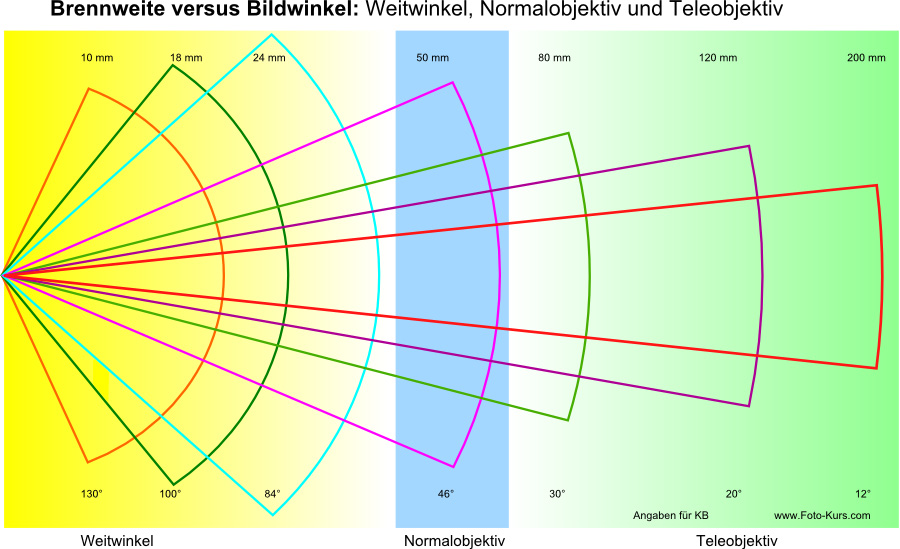
\includegraphics[width=0.7\textwidth]{abb1} 
	\caption[Brennweite und Bildwinkel]{Brennweite und Bildwinkel\footnotemark}\label{fig:abb1}
\end{figure}
\footnotetext{Quelle: https://www.foto-kurs.com/objektiv-digitalkamera.htm}
\begin{itemize}
	\item Normalobjektiv
		\begin{itemize}
		\item Das Normalobjektiv entspricht im Grunde dem menschlichen Blickwinkel, und wird meist als natürlich empfunden.\citep{normalobjektiv}
		\end{itemize}
	\item Weitwinkel
		\begin{itemize}
		\item Wie man auf der obigen Abbildung sehen kann, haben Weitwinkelobjektive einen breiten Bildwinkel, somit sieht man mehr vom Bild.\citep{normalobjektiv}
		\end{itemize}
	\item Teleobjektiv
		\begin{itemize}
		\item Teleobjektive nehmen Objekte mit einem kleinen Blickwinkel aus großer Entfernung auf. Teleobjektive haben daher einen eher kleinen Schärfentiefenbereich, was sich beispielsweise für Interviews schlecht eignet.\citep{tele}
\end{itemize}
\end{itemize}
\paragraph{Schärfentiefe}
\leavevmode \\
"Die Schärfentiefe ist das Maß für den in einem Bild scharf abgebildeten Bereich." (Jörg Jovy, 2017, S. 223)\newline
Der Sinn der Schärfentiefe ist, ein Objekt oder Motiv vom Hintergrund abzuheben, also es schärfer darstellen zu lassen als den Hintergrund.\citep{scharf}\newline
Die Schärfentiefe kann durch drei Parameter eingestellt werden:
\begin{itemize}
	\item Sensorgröße
	\item Blende
	\item Brennweite
\end{itemize}
Wie vorhin erklärt, hat der Sensor auch einen Einfluss auf die Schärfentiefe, nämlich je größer der Sensor ist, desto mehr Spielraum bietet sich.\newline
Je weiter die Blende geöffnet ist, desto geringer ist die Schärfentiefe. Zuletzt kann noch die Brennweite eingesetzt werden, um eine geringe Schärfentiefe zu erzeugen. Je näher man an ein Objekt heranzoomt, desto unschärfer wird der Hintergrund.\citep{scharfZwei}\newline 
Bei allen drei Videos wurden Zoomobjektive verwendet. Zoomobjektive haben eine variable Brennweite, das heißt man muss sich nicht auf eine fixe Brennweite festlegen, sondern kann selbst entscheiden welche Brennweite man haben möchte. Bei dem Dreh der Videos kam das Canon Objektiv EF-S 18-135mm f/3.5-5.6 IS USM zum Einsatz. Durch das Zoomobjektiv war es möglich das Filmen flexibel zu gestalten.\newline
Beim Dreh des Interviews mit dem Abteilungsvorstand wurde die Brennweite nicht berücksichtigt und somit hat die nötige Schärfentiefe im Bild gefehlt. Dies wurde anschließend in der Post Production nachträglich nachbearbeitet. Bei dem Tag der offenen Tür Video konnte mit dem Wissen, dass die Brennweite auch einen Einfluss auf die Schärfentiefe hat, die optimale Schärfentiefe erzielt werden.
\section{Beleuchtung}
In der Videografie wird die Belichtungszeit in der Bildrate vorgegeben, wohingegen sie in der Fotografie zwischen mehreren Stunden und wenigen Sekunden liegen kann.
Die richtige Belichtungszeit kann man sich mit folgender Formel berechnen: \textit{Belichtungszeit = 1: Framerate x 2}. Nimmt man nun mit 25 Bildern pro Sekunde auf, ergibt sich eine Belichtungszeit von 1:50 = 1/50 s. Würde man die Belichtungszeit verkürzen, z.B. auf 1/125 s, dann würde das Bild zwar schärfer werden, aber dann würde die Gefahr bestehen, dass der sogenannte Moir\'{e} Effekt eintritt. Der Moir\'{e} Effekt ist ein Bildfehler, der bei bewegten Bildern ein Flimmern erzeugt. \begin{quote}Moir\'{e} tritt überall da auf, wo feine Muster oder Raster in einem gegeneinander verschobenen Winkel übereinanderliegen und sich gegenseitig beeinflussen. (Jörg Jovy, 2017, S. 211)\end{quote}
\begin{figure}[H]
	\centering
	
\includegraphics[width=0.8\textwidth]{abb2} 
	\caption[Moir\'{e}-Effekt]{Moir\'{e}-Effekt\footnotemark}
\end{figure}
\footnotetext{Quelle: https://de.wikipedia.org/wiki/Moir\%C3\%A9-Effekt\#/media/File:Moir\%C3\%A92.png}
Bei der Beleuchtung muss man drei Positionen von den Lichtquellen der Belichtung unterscheiden. Das Licht, das von vorne auf den Gegenstand kommt, nennt man Gegenlicht. Das Licht, das von der Seite kommt, wird als Streiflicht bezeichnet, und als drittes Licht wird das Auflicht verwendet, welches von hinten auf das Objekt scheint.\citep{beleuchtung}
\begin{figure}[H]
	\centering
	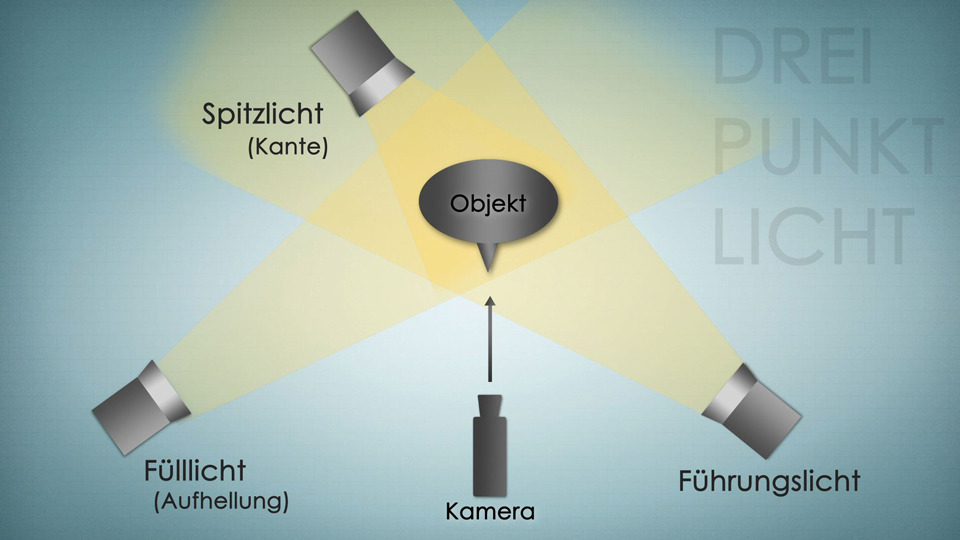
\includegraphics[width=0.7\textwidth]{abb3}
	\caption[Zusammenspiel der Lichter]{Zusammenspiel der Lichter\footnotemark}\label{fig:abb3}
\end{figure}
\footnotetext{Quelle: http://www.filmmachen.de/tipps-und-tricks/licht/3-punkt-beleuchtung}
Wie man auf der Abbildung \ref{fig:abb3} erkennen kann, ist es wichtig, wie die Lichter im Verhältnis zueinander stehen. Das Führungslicht, oder auch Hauptlicht genannt, dient dazu, die Szene generell aufzuhellen. Durch die Verwendung des Führungslichts entstehen Schatten, die wiederrum mit dem Fülllicht reduziert werden. Um den Gegenstand auch optisch vom Hintergrund abzuheben, kommt das sogenannte Spitzlicht zum Einsatz. \citep{lichter}
\paragraph{Softbox}
\leavevmode \\
Um den Schauplatz genügend auszuleuchten, wurden für alle vier Videos LED Scheinwerfer verwendet. Um keine harten Schatten zu erzeugen, wurden noch zusätzlich Softboxen verwendet.\newline
Eine Softbox ist im Grunde eine Hülle, bei der die Innenseite silber ist und welche dadurch das Licht wie ein Reflektor nach vorne reflektiert. Anschließend geht das Licht durch den "Front - Diffuser", was
ein lichtdurchlässiges Gewebe ist, der das Licht streut, und es so diffuser erscheinen lässt. Dadurch wird auch die Helligkeit reduziert und aufgrund der großen Fläche wird das Licht weicher, wodurch die Schatten diffuser werden.\citep{softbox}\newline
Bei dem Interview mit dem Abteilungsvorstand wurde jedoch keine 3-Punkt-Beleuchtung angewandt. Es wurde mit zwei Lichtquellen gearbeitet, um kein gekünsteltes Video zu erstellen. Die zwei Lichtquellen sollen nur dazu dienen, die Szene generell aufzuhellen und, um eventuelle Schatten auszugleichen. Es soll natürlich wirken und dem Betrachter nicht das Gefühl geben, dass es gestellt ist.  Dieses Set wurde ebenfalls bei dem Dreh des Quiz mit dem Absolventen und dem Schüler der zweiten Klasse angewandt, um auch hier ein natürliches Ergebnis zu erzeugen.
\section{Mikrofone}
\subsection{Richtcharakteristik}
\begin{quote}
"Die Richtcharakteristik definiert, aus welcher Richtung das Mikrofon den Schall besonders empfindlich aufnimmt. Stark vereinfacht gesagt: Aus welcher Richtung aufgenommen wird." (https://www.delamar.de/mikrofon/richtcharakteristik-mikrofon-22647/ [Zugriff: 17.03.2018])
\end{quote}
\subsubsection{Kugelcharakteristik}
Bei der Kugelcharakteristik wird der Schall von allen Richtungen aufgenommen, das heißt es wird von keiner bevorzugten Richtung aufgenommen. Das Problem, was dadurch entsteht, ist, dass die Rückkoppelanfälligkeit sehr hoch ist, wodurch Mikrofone mit einer Kugelcharakteristik schlecht für Bühnen geeignet sind.\citep{kugel}
\begin{figure}[H]
	\centering
	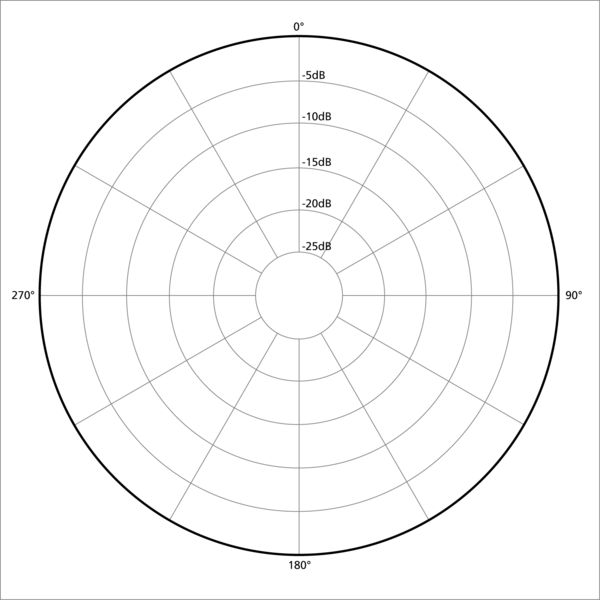
\includegraphics[width=0.4\textwidth]{abb4} 
	\caption[Kugel]{Kugel\footnotemark}
\end{figure}
\footnotetext{Quelle: https://www.delamar.de/mikrofon/richtcharakteristik-mikrofon-22647/}
\subsubsection{Nierencharakteristik}
Die Niere nimmt, im Gegensatz zur Kugelcharakteristik, aus einer bevorzugten Richtung auf. Im Gegensatz zu der Kugelcharakteristik, bei der der Schall von allen Seiten aufgenommen wird, wird er bei der Niere nur von einer Seite aufgenommen, meistens von vorne. Der Schall wird von den Seiten nur sehr leise bis gar nicht aufgenommen. Der Vorteil der Niere ist, dass sie rückkopplungsfester, als die Kugel ist und sie so auch beispielsweise bei Konzerten verwendet werden kann. Der Nachteil der Niere ist der sogenannte Nahbesprechungseffekt.\citep{naheffekt}\citep{kugel} Das bedeutet: "Ab einer gewissen Nähe der Schallquelle werden die tieffrequenten Anteile dominanter." (https://www.delamar.de/faq/nahbesprechungseffekt-34021/ [Zugriff: 17.03.2018])
\begin{figure}[H]
	\centering
	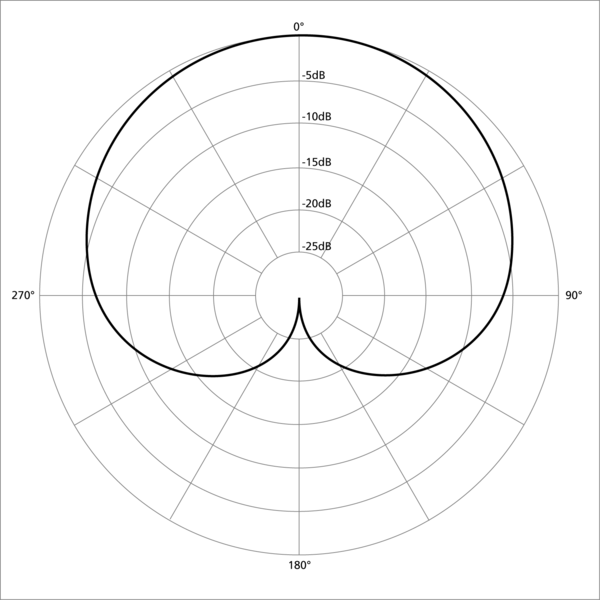
\includegraphics[width=0.4\textwidth]{abb5} 
	\caption[Niere]{Niere\footnotemark}
\end{figure}
\footnotetext{Quelle: https://www.delamar.de/mikrofon/richtcharakteristik-mikrofon-22647/}
\subsubsection{Keule/Superniere}
Keule beziehungsweise Superniere sind Charakteristiken, die von der Niere abgeleitet sind. Die Fläche der Keule ist im Gegensatz zu der Niere etwas schmaler. Das hat die Auswirkung, das von den Seiten weniger aufgenommen wird. Dadurch sind Mikrofone mit einer Keule oder Superniere hinten empfindlicher.\citep{kugel} "Dennoch haben sie die höchste Rückkopplungsfestigkeit." (https://www.delamar.de/mikrofon/richtcharakteristik-mikrofon-22647/ [Zugriff: 17.03.2018])
\begin{figure}[H]
	\centering
	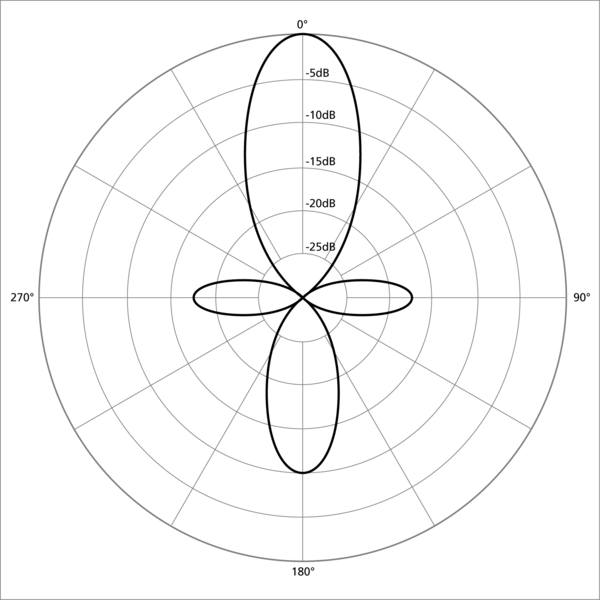
\includegraphics[width=0.4\textwidth]{abb6} 
	\caption[Keule]{Keule\footnotemark}
\end{figure}
\footnotetext{Quelle: https://www.delamar.de/mikrofon/richtcharakteristik-mikrofon-22647/}
\subsubsection{Acht}
Die sogenannte Achtcharakteristik nimmt den Schall von vorne und hinten auf, jedoch nur minimal von den Seiten. Diese Charakteristik hat die Verwendung bei der M/S-Stereofonie.\citep{kugel}\newline
Bei der M/S-Stereofonie, oder auch Mid/Side-Stereofonie, werden die Audiosignale mittig und von der Seite aufgenommen. In der Mitte befindet sich ein Mikrofon mit einer Nierencharakteristik, wohingegen die Seitensignale mit einer Achtcharakteristik aufgenommen werden. Die Seitensignale nehmen die Schallquellen aus unterschiedlichen Richtungen auf und sind so mit einem menschlichen Ohr zu vergleichen.\citep{ms}
\begin{figure}[H]
	\centering
	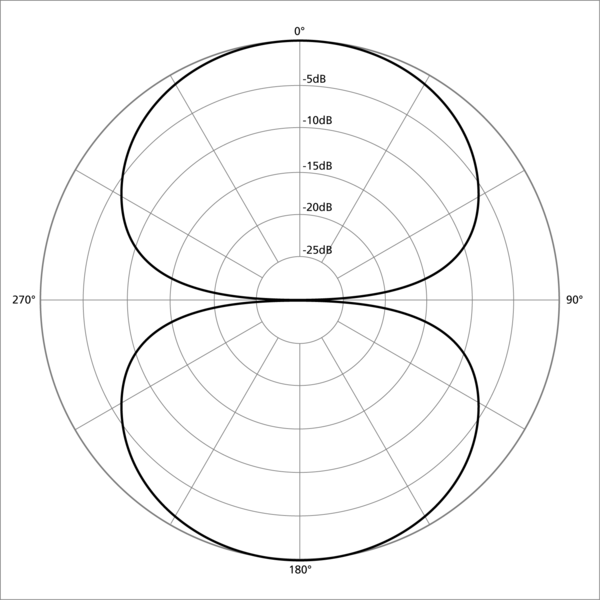
\includegraphics[width=0.4\textwidth]{abb7} 
	\caption[Acht]{Acht\footnotemark}
\end{figure}
\footnotetext{Quelle: https://www.delamar.de/mikrofon/richtcharakteristik-mikrofon-22647/}
\subsection{Kondensatormikrofon}
"Ein Kondensatormikrofon wandelt Schall in ein elektrisches Signal." (https://www.delamar.de/faq/kondensatormikrofon-34728/ [Zugriff: 17.03.2018])\newline
Bei einem Kondensatormikrofon treffen die Schallwellen zuerst auf die Membran, was eine leitende Folie ist, die mit Gold bedampft ist. Dies verbessert die  Leitfähigkeit des Mikrofons, was die Luftdruckschwankungen in mechanische Schwingungen umwandelt. Anschließend wird sie in elektrische Spannung umgewandelt und über die XLR-Buchse wieder ausgegeben.\citep{kondensator}
\begin{figure}[H]
	\centering
	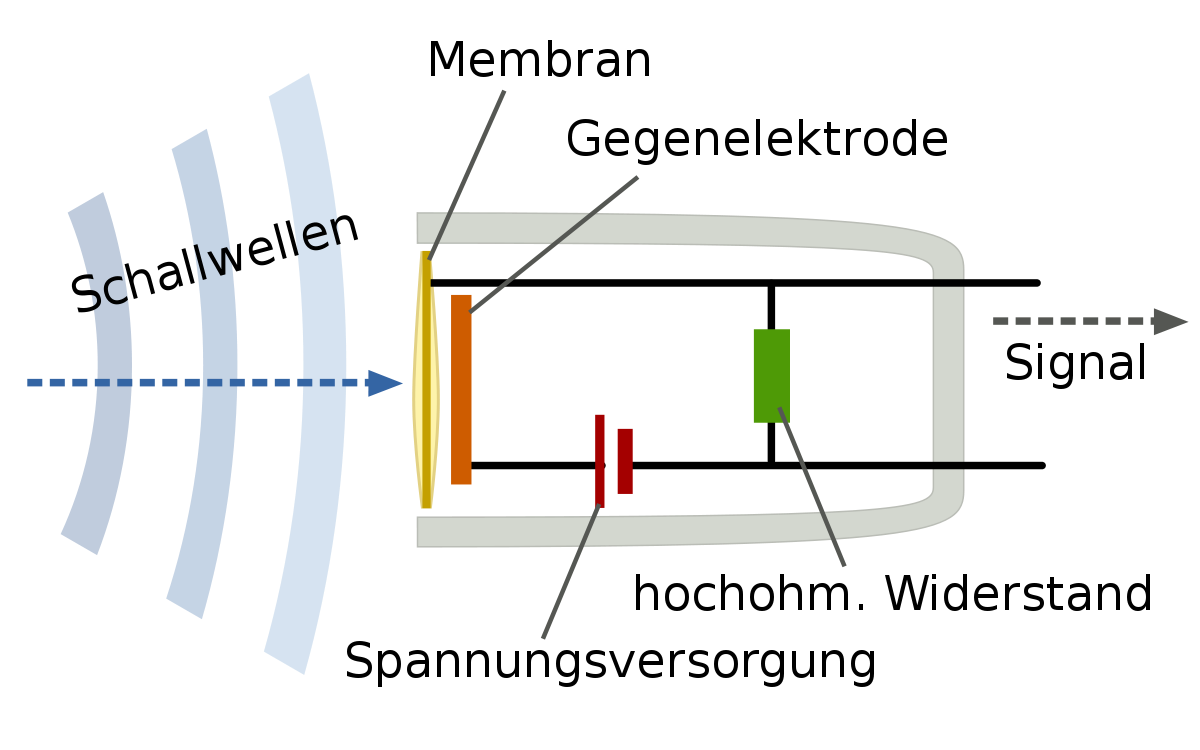
\includegraphics[width=0.6\textwidth]{abb8} 
	\caption[Kondensatormikrofon]{Kondensatormikrofon\footnotemark}
\end{figure}
\footnotetext{Quelle: https://de.wikipedia.org/wiki/Kondensatormikrofon\#/media/File:Kondensatormikrofon.svg}
\subsection{Dynamisches Mikrofon}
\begin{quote}
"Bei diesem Mikrofontyp wird das Signal durch elektromagnetische Induktion erzeugt. Kurz: Der Schall trifft auf die Membran des Mikrofons und regt sie zu mechanischen Schwingungen an, die durch eine mit der Membran verbundene Spule in elektrische Spannung umgewandelt werden. Und diese kommt dann aus der (XLR-)Buchse des Mikrofons." (https://www.delamar.de/faq/dynamisches-mikrofon-34718/ [Zugriff: 17.03.2018])
\end{quote} 
\begin{figure}[H]
	\centering
	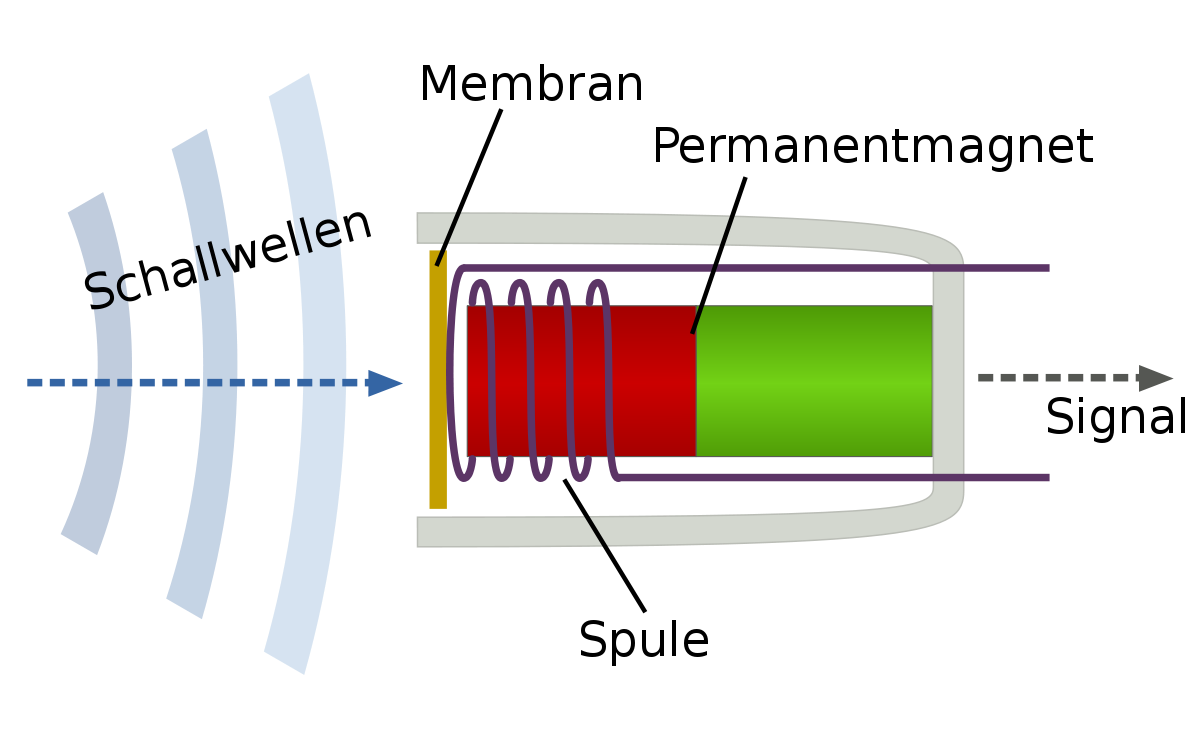
\includegraphics[width=0.6\textwidth]{abb9} 
	\caption[Dynamisches Mikrofon]{Dynamisches Mikrofon\footnotemark}
\end{figure}
\footnotetext{Quelle: https://de.wikipedia.org/wiki/Dynamisches\_Mikrofon\#/media/File:Tauchspulenmikrofon.svg}
\paragraph{Interview mit Abteilungsvorstand}
\leavevmode \\
Bei der Aufnahme des Videos mit dem Abteilungsvorstand Dr. Hager wurde das t-bone GZ 400 Grenzflächen-Mikrofon verwendet. Das Mikrofon arbeitet mit der Richtcharakteristik Halbniere. Das Mikrofon wurde in die Mitte des Tisches platziert, um die Stimmen der Interviewerin und des Abteilungsvorstandes einzufangen.\newline
Bei dem Video wurden bewusst keine Ansteckmikrofone verwendet, um nicht das typische Interview-Bild widerzuspiegeln, wo die Mikrofone an den Personen angesteckt werden und man diese dann auch im Video sieht.
\paragraph{Tag der offenen Tür}
\leavevmode \\
Bei dem Tag der offenen Tür Video wurde eine Angel für die Aufnahme der Interessenten verwendet. Hierfür wurde eine Keule beziehungsweise eine Superniere eingesetzt. Dies war deswegen notwendig, da am Tag der offenen Tür viele Hintergrundgeräusche vorhanden waren. Hätte man mit einer Kugelcharakteristik aufgenommen, würde man die Hintergrundgeräusche auch hören, im Gegensatz zu der Keule, welche hauptsächlich von vorne aufnimmt und Hintergrundgeräusche ausblendet.
\paragraph{Video mit einem Absolvent}
\leavevmode \\
Beim Quiz mit dem Absolventen und dem Schüler der zweiten Klasse wurde, wie beim ersten Interview, das Grenzflächen-Mikrofon verwendet.
\section{Planung und Vorbereitung}
Für die Planung eines Videos benötigt man meistens viel Zeit, um auch ein gutes Ergebnis zu erzielen. Bevor es an das bekannte Drehbuch geht, muss man vorerst noch drei andere Schritte berücksichtigen, nämlich die sogenannte Logline, das Expos\'{e} und das Treatment. Erst nach diesen Schritten ist es sinnvoll das Drehbuch zu schreiben.\citep{planung}
\subsection{Logline}
Die Logline ist, vereinfacht gesagt, die Idee zum Film oder zum Video. Die Logline besteht meistens nur aus einem Satz und soll nur einen groben Überblick über den Film oder des Videos preisgeben.\citep{logline}
\begin{figure}[H]
	\centering
	
\includegraphics[width=1.0\textwidth]{abb26} 
	\caption{Logline des Tag der offenen Tür Videos}
\end{figure}
\subsection{Expos\'{e}}
Das Expos\'{e} besteht meist nur aus ein paar Skizzen, wobei folgende Themen behandelt werden: das Thema selbst, die Besonderheiten des Videos oder Films, die Protagonisten, Drehorte und sonstige Herausforderungen. Das Expos\'{e} soll den Mitarbeitern dazu dienen, weitere Entscheidungen leichter zu treffen.\citep{expose}
\subsection{Treatment}
Das Treatment ist mehr oder weniger der Vorgänger des Drehbuchs. Ein Treatment beinhaltet schon kurze Dialoge zu bestimmten Szenen und eine szenengenaue Auflösung zum Film oder zum Video.\citep{treatment}
\subsection{Drehbuch}
Das Drehbuch ist, im Vergleich zum Treatment, komplett ausgearbeitet, das heißt, es liegt ein kompletter Produktionsleitfaden vor, wobei jede Szene ausgearbeitet ist. Weiters werden wichtige Einstellungen in Bildszenen dargestellt. Adobe stellt die Software \textit{Story} zur Verfügung, mit der man Drehbücher erstellen kann.\citep{drehbuch}\newline
Story ist eine Software von Adobe, mit der man Drehbücher erstellen kann. Bei der Erstellung kann man ein vorgefertigtes Template auswählen und anschließend kann man schon das Drehbuch verfassen. Bei der Erstellung des Drehbuchs kann man zwischen Scene Heading, Action, Character, Parenthetical, Dialog, Transition, Speaking Extra, Shot und General auswählen. Diese Elementtypen sind auch schon dementsprechend formatiert und man muss weder etwas einrücken, noch sonstige Formatierungen einstellen.\citep{drehbuchZwei}\\ 
Da nur Interviews geplant wurden und man bei Interviews keine Szenen planen kann, wurde das Expos\'{e}, das Treatment und das Drehbuch übersprungen. Jedoch wurde eine Logline und das Storyboard verfasst und zusätzlich wurde noch ein Fragenkatalog pro Video erstellt. 
\subsection{Storyboard}
Ein Storyboard ist eine visualisierte Veranschaulichung von dem Konzept, das man sich zuvor überlegt hat.\citep{storyboard} Um die korrekte Ausführung der Videos zu gewährleisten, wurden Storyboards angefertigt. Diese wurden mit der Online Plattform "Storyboard That"\citep{storyboardLink} erstellt und schließlich als PDF - Format exportiert.
Im Storyboard wurden die Szenen bildlich dargestellt, was das Team im weiteren Verlauf unterstützte, da es dadurch grobe Fehler vermeiden konnte.
Das Online - Tool ermöglichte es zwischen verschiedensten Szenen, Charakteren und Kategorien auszuwählen, wodurch vereinfacht, verschiedenste Szenen dargestellt werden konnten. 
\begin{figure}[H]
\begin{center}
	\fbox{\includegraphics[scale=0.30]{abb10}}
	\caption{Storyboard des Interviews mit dem Abteilungsvorstand}
\end{center}
\end{figure}
\section{Setting}
Beim Aufbau des Sets wurde auf das Drehbuch und das Storyboard referenziert. Hierbei wurde auch die Location berücksichtigt, da für den Aufbau eines Videos mit Greenscreen ein anderes Set von Nöten war, als bei einem Video am Gang in der Schule. Weiters musste überlegt werden, wie die Kameras und Lichter platziert werden müssen. Bevor es zum eigentlichen Dreh kam, wurde das Setting im Vorhinein ausreichend getestet, um später beim wirklichen Dreh, Fehler zu vermeiden. Weiters wurden zusätzlich verschiedene Mikrofone getestet, um für die jeweilige Situation das optimale Mikrofon zu verwenden.
\section{Post Production}
\subsection{Aufnahmeformate}
Bei der Auswahl des Aufnahmeformates muss man sich im Klaren sein, mit welchem Codec man aufnehmen möchte. Hierbei muss man zwischen Codecs und Containern unterscheiden. Container, welche den Videostream mittels eines Codecs digitalisieren, speichern die Videodaten auf dem Speicherchip. Audio Video Interleave (AVI), QuickTime (MOV) oder Moving Pictures Expert Groups (MPEG) sind zum Beispiel solche Containerformate. Ein Codec wandelt analoge Bilder in digitale Datenströme um. Bei der Codierung wird das Bild komprimiert, was wiederum mehr Speicherplatz zur Verfügung stellt. DivX, QuickTime H.264, Apple ProRes, Panasonic AVC-Intra oder Avid DNxHD sind typische Codecs.\citep{aufnahmeformate}\newline
Die Komprimierung des Videosignals erfolgte bei allen vier Videos mittels dem H.264 Codec im QuickTime (MOV) Container. 
\paragraph{MPEG}
\leavevmode \\
"MPEG ist ein standardisiertes Kompressionsverfahren, das sich speziell zur Datenreduktion von Bewegtbildern eignet." (https://www.film-tv-video.de/term-word/mpeg/ [Zugriff: 26.03.2018]) MPEG lässt dem Gerätehersteller freie Wahl, bezüglich der Entscheidung der Datenerzeugung. Jedoch legt MPEG das Datenformat und die Dekodierung vor. Was noch beachtet werden muss, ist, dass schlussendlich ein normgerechter MPEG-kodierter Datenstrom entstehen muss, der mit einem MPEG-Decoder gelesen und wiedergegeben werden kann. Bei dem MPEG Standard setzen sich die Einzelbilder einer Videosequenz aus einer Folge von I-, B- und P-Frames zusammen. Diese Aufeinanderfolgung wird Group of Pictures, kurz GOP, genannt. Eine Group of Pictures muss mindestens ein I-Frame enthalten. I-Frames sind Indexbilder, welche die wichtigsten Bildinformationen enthalten. "B-Frames sind  bidirektionale Bilder, also Frames, die nur die Unterschiede eines Bildes zum vorhergehenden oder folgenden Bild beinhalten." (https://www.film-tv-video.de/term-word/mpeg/ [Zugriff: 26.03.2018]) P-Frames sind Predicted Frames. Predicted Frames werden aus den vorherigen I-Frames berechnet.\newline
\begin{figure}[H]
	\centering
	\includegraphics[width=0.8\textwidth]{abb27} 
	\caption[Group of Pictures]{Group of Pictures\footnotemark}
\end{figure}
\footnotetext{Quelle: https://www.itwissen.info/GOP-group-of-picture.html}
\leavevmode \\
Der QuickTime Container ist im Grunde, wie das MPEG Containerformat aufgebaut. Jedoch ist QuickTime ein eigenes Containerformat von Apple.\citep{mpeg}
\subsection{Kompressionsverfahren}
Bei der Bildkompression werden die Bildinformationen in 4x4, 8x8 oder 16x16 Pixeln zusammengefasst. "In einzelnen Bildern und zwischen aufeinanderfolgenden Bildern werden dann sich wiederholende Daten identifiziert." (Jörg Jovy, 2017, S. 117)\newline
Nun können die wiederholenden Informationen gefiltert und weggelassen werden. Bei dem MPEG-2 Container wird zum Beispiel nur jedes zwölfte Bild komplett gespeichert, wobei bei den anderen Bildern nur Teile beziehungsweise Veränderungen gespeichert werden. Da nur jedes zwölfte Bild komplett gespeichert wird, ist das Risiko enorm groß, dass Artefakte, also Bildfehler, entstehen können. Die sogenannten Artefakte entstehen bei der Umwandlung von digitalen Bildern in analoge Bildsignale.\citep{kompression}
\subsection{Schnittprogramme}
\paragraph{Lightworks}
\leavevmode \\
Lightworks ist ein lizenzfreies Videoschnittprogramm, das auf Windows, Linux und auf IOS Betriebssystemen verwendet werden kann. Lightworks bietet nicht nur die freie Version, sondern auch eine Pro Version. Die freie Version bietet dem User eine Vielzahl an importierbaren Formaten, wie zum Beispiel Apple Pro Res, AVC-Intra 50, MPEG-2 Long GOP und vieles mehr. Weiters kann man in Lightworks seine Videos mit dem Codec H.264 mit der Auflösung 1280x720p kodieren.\citep{lightworks}\citep{lightworksZwei}
\paragraph{Adobe Premiere Pro}
\leavevmode \\
Adobe Premiere Pro ist eine kostenpflichtige Software, welche aber eine Vielzahl von Funktionalitäten bietet. Im Gegensatz zu Lightworks bietet Adobe Premiere Pro eine freie Auswahl, welche Formate man importieren möchte. Weiters bietet Premiere Pro eine umfangreiche Dokumentation. Zusätzlich sind Adobe Programme ähnlich aufgebaut und sind so einfach miteinander zu verknüpfen, wie zum Beispiel Premiere Pro mit Adobe After Effects.\citep{premiere}
\subsection{Schnitt}
Bevor mit dem Schnitt begonnen werden kann, muss zunächst das Projektformat festgelegt werden. Bei Erstellung einer neuen Sequenz können folgende Parameter eingestellt werden
\begin{itemize}
	\item Bilder pro Sekunde
	\item Pixel - Seitenverhältnis
	\item Audio-Samplerate
	\item Bildgröße in Pixeln
	\item Render-Qualität
\end{itemize}
Hat man diese Eigenschaften festgelegt, kann man auch schon mit dem Schnitt beginnen. Es gibt drei Arten des Filmschnitts. Den Rough Cut oder schnelle Schnitt, 3-Punkt-Schnitt oder der exakte Schnitt und den 4-Punkt-Schnitt oder Zeitinterpolation.\citep{schnitt}
\subsection{Blenden}
Blenden signalisieren dem Zuschauer, dass es sich um eine neue Szene handelt. Blenden sind ein wertvolles Mittel, um den Film oder das Video angenehmer zum Ansehen machen. In Adobe Premiere gibt es eine Vielzahl an unterschiedlichen Blenden, bei denen man sich vorher überlegen sollte, was man mit der Blende bewirken will. In Premiere gibt es nicht nur typische Blenden, wie "Weiche Blende" oder "Filmblende", sondern auch Effektblenden. Die meisten Effektblenden werden jedoch nicht eingesetzt, da sie den Zuschauer nicht besonders ansprechen. Die einzige Effektblende, die verwendet wird, ist die Wipe oder auch Schiebeblende genannt.\citep{blende}
Bei dem Schnitt des Tag der offenen Tür Videos kam eine Blende zum Einsatz, nämlich die "Weiche Blende". Die weiche Blende wurde für die Übergänge verwendet von einer Frage zu der Antwort oder zum Ausblenden eines Textes.\newline
Bei dem Schnitt des Videos mit dem Absolventen kamen drei verschiedene Blenden zum Einsatz:
\begin{itemize}
	\item Wegschieben
	\item Filmblende
	\item Einzoomen \& Auszoomen
\end{itemize}
Die Wegschieben Blende ist sozusagen die Hauptblende und dient dazu, von einer einer Szene zur nächsten überzugehen. Die Filmblende blendet die erzielten Punkte ein und die Ein- und Auszommen Blende wurde für das Einblenden der Antworten genutzt.
\subsection{Color Correction}
Mithilfe der Lumetri-Scopes und der Farbkorrektur in Premiere Pro kann man die Farbe im Bild korrigieren. Einerseits gibt es die Lumetri-Scopes, bei denen man auf einen Blick erkennen kann, welche Farbinformationen nicht so dominant sind, ob das Bild über- oder unterbelichtet ist und wie die Helligkeitsverteilung im Bild ist. Und zum anderen gibt es die Farbkorrektur "Lumetri-Farbe" mit der man die oben genannten Eigenschaften verbessern kann.\citep{cc}
\paragraph{Vektorskop}
\leavevmode \\
"Das Vektorskop gibt Auskunft über die Farbverteilung im Bild." (Jörg Jovy, 2017, S. 523) Auf dem Vektorskop sind die Grundfarben aus dem RGB und dem CMYK Farbraum abgebildet. Also: Rot, Grün, Blau, Cyan, Magenta, Yellow. Je weiter der Signalpunkt sich vom Zentrum entfernt, desto höher ist die jeweilige Farbsättigung. Hätte man ein Schwarz-Weiß-Bild würde man einen Punkt in der Mitte sehen.\citep{vektorskop}\newline
Wie man auf der Abbildung \ref{fig:abb22} sehen kann, hat das Bild eine hohe Farbsättigung von Yellow und Rot, wohingegen es nur wenige Blauanteile hat.
\begin{figure}[H]
	\centering
	\includegraphics[width=1.0\textwidth]{abb22} 
	\caption{Vektorskop}\label{fig:abb22}
\end{figure}
\paragraph{Histogramm}
\leavevmode \\
Das Histogramm zeigt die Häufigkeitsverteilung von Helligkeit und Farbe, die im Bild vorkommt. Weiters zeigt das Histogramm, ob das Bild korrekt belichtet wurde. Das Histogramm geht von 0,0,0 für RGB Schwarz bis 255,255,255 für RGB Weiß. Die Schatten befinden sich beim Histogramm unten, also in Richtung 0,0,0, wobei man die Lichter oben, also in Richtung 255,255,255 findet.\citep{histogramm}\newline
Bei dem Histogramm sieht man, wie bei dem Vektorskop, dass die Farben Yellow und Rot eindeutig dominieren. 
\begin{figure}[H]
	\centering
	\includegraphics[width=1.0\textwidth]{abb21} 
	\caption{Histogramm}
\end{figure}
\paragraph{Waveform-Monitor}
\leavevmode \\
Der Waveform-Monitor zeigt die Helligkeitsverteilung im Bild. Die Helligkeit wird als Häufigkeitsverteilung wiedergegeben, wobei 100\% Weiß einen Messwert von 100 IRE entsprechen. "IRE ist die international übliche Skalierung." (Jörg Jovy, 2017, S. 522)\newline
0 IRE entsprechen daher Schwarz. Mithilfe des Waveform-Monitors kann man die sogenannten Lichter, Mitten und Tiefen einfach analysieren.\citep{waveform}\newline
Wie man auf der Abbildung \ref{fig:abb20} sehen kann, reichen die Tiefen bis zu dem Null Wert, das heißt es werden auch die Schatten völlig ausgeschöpft. Die Mitten sollten zwischen 50 und 70\% liegen und befinden sich auch, wie man hier sehen kann, in dem Bereich.\citep{waveformZwei}
\begin{figure}[H]
	\centering
	\includegraphics[width=1.0\textwidth]{abb20} 
	\caption{Waveform-Monitor}\label{fig:abb20}
\end{figure}
\subsection{Lumetri-Farbkorrektur}
\paragraph{Einfache Korrektur}
\leavevmode \\
Bei der einfachen Korrektur können grundlegende Verbesserungen vorgenommen werden:\citep{farbkorrektur}
\begin{itemize}
	\item Weißabgleich
	\item Farbton
	\item Sättigung
\end{itemize}
\paragraph{Kreativ}
\leavevmode \\
Im Kreativ-Bereich kann dem Video ein bestimmter Look verpasst werden, wie zum Beispiel ein CineSpace Look. Weiters kann der Scharfzeichner, die Dynamik und die Sättigung eingestellt werden\citep{farbkorrektur}
\paragraph{Kurven}
\leavevmode \\
Bei den Kurven kann man zwischen RGB-Kurven und Farbtonsättigungskurven unterscheiden.\newline
Mit den RGB-Kurven kann die Luminanz und die Farbtonbereiche des Bildes angepasst werden. Man kann die Kurve entweder für alle drei RGB-Kanäle gleichzeitig anpassen, oder man kann es auch für die einzelnen RGB-Farbkanäle anpassen, also für Rot, Grün und Blau.\newline
Bei der Farbtonsättigungskurve kann die Sättigung angepasst werden. Man kann die Sättigung bestimmter Farbtöne verringern und erhöhen.\citep{farbkorrektur}\newline
Wie man anhand der Abbildung \ref{fig:abb19} sehen kann, ist, dass die rote Farbtonsättigung erhöht wurde. Dies hatte diesen Effekt, dass die Gesichtsfarbe der Person in einen rötlicheren Farbton veränderte.
\begin{figure}[H]
	\centering
	\includegraphics[width=1.0\textwidth]{abb19} 
	\caption{Farbtonsättigungskurve}\label{fig:abb19}
\end{figure}
\paragraph{Farbräder}
\leavevmode \\
Bei den Farbrädern können die Schatten, Mitteltöne und Glanzlichter angepasst werden.\citep{farbkorrektur}
\subsection{Masken}
In Adobe Premiere Pro kann man mit Masken einen bestimmten Bereich markieren, den man anschließend verändern möchte. In der folgenden Abbildung \ref{fig:abb28} kann man die Verwendung der Maske von dem Interview mit dem Abteilungsvorstand sehen. 
Hierbei wurde die Maske mit einem Weichzeichner versehen, um den Hintergrund unscharf wirken zu lassen. Die Masken können mit einem Ellipsen-Werkzeug, Rechteck-Werkzeug oder einem Zeichenstift erstellt werden. Für die abgebildete Maske kam der Zeichenstift in Verwendung. Nach dem die Maske gezeichnet wurde, kann man die Maske frame für frame bewegen. In diesem Fall konnte sich die Maske nicht automatisch mitbewegen, da sich der Hintergrund von der Maske nicht abgehoben hat. Somit musste die Maske manuell nachbearbeitet werden.\newline
Um einen flüssigen Übergang zwischen dem Maskenauswahlrahmen und dem Bereich außerhalb der Auswahl zu erzeugen, kann man eine weiche Kante anwenden.\citep{masken}\begin{quote}Die weichen Kanten glätten den Maskenauswahlrahmen, sodass die Maske mit dem Bereich außerhalb der Auswahl verschmilzt und ein ästhetisch ansprechendes Ergebnis entsteht." (https://helpx.adobe.com/de/premiere-pro/using/masking-tracking.html [Zugriff: 31.03.2018])\end{quote}
Weiters wurde die Maske bei dem Tag der offenen Tür Video angewandt. Dies war deswegen notwendig, da aufgrund des ständigen Lichtwechsels die Gesichtsfarbe der Personen sich immer änderte. 
\begin{figure}[H]
	\centering
	\includegraphics[width=1.0\textwidth]{abb28} 
	\caption{Maskenpfad des Interviews mit dem Abteilungsvorstand}\label{fig:abb28}
\end{figure}
\subsection{Geschwindigkeitseffekte}
Am Tag der offenen Tür wurde der Eingangsbereich der Schule für etwa 20 Minuten gefilmt. Dieses Video wurde schließlich für das Tag der offenen Tür Video verwendet. Um den Zuschauer kein 20 Minuten langes Video anschauen zu lassen, wurde die Geschwindigkeit des Videos beschleunigt, und somit ein Zeitraffer erzeugt. Mit einem Rechtsklick auf die Spur kann man auch schon die Eigenschaft "Geschwindigkeit/Dauer" auswählen, bei der man die Geschwindigkeit beschleunigen oder verlangsamen kann.\citep{effekte}
\subsection{Musik}
Bei dem Tag der offenen Tür Video und dem Quiz wurde lizenzfreie Musik eingebunden. Diese stammt von Soundcloud. Die Verwendung von Musik lockert das Schauen eines Videos auf und löst beim Menschen Spannung, Mitleid, Angst oder Entspannung aus. Weiters dient die Musik geräuschlose Szenen zu überbrücken und sie so angenehmer machen.\citep{musik}
\subsection{Export}
Bei dem Export eines Videos in Adobe Premiere muss man sich zuerst für ein Format entscheiden, in dem man das Video exportieren möchte. Heutzutage wird der H.264 von allen Browsern unterstützt und deswegen wurden auch die Videos in dem Codec kodiert. Jedoch unterstützen veraltete Mozilla Firefox Browser keinen H.264 Codec, sondern den Web.m Codec. Um zu gewährleisten, dass sich jeder User die Videos ansehen kann, wurden die Videos auch im Web.m Codec kodiert. Da Adobe Premiere den Web.m Codec nicht implementiert hat, war es notwendig diesen mittels einer msi Datei einzubinden.\citep{export}\citep{exportZwei}
\input{video/herausforderungen.tex}

\section{Interview mit einem Fachmann}
\subsection{Idee}
Es sollte ein Interviewvideo mit einem passionierten Medientechniklehrer gedreht werden, um den Usern, der erstellten Plattform, einen tiefen Einblick in die Medientechnik zu bieten. Dabei wird auch an Fragestellungen aus dem Animationsvideo angeknüpft, jedoch wird auf diese ausführlicher und detailreicher eingegangen. Die Aufnahme bietet durch Verwendung eines Green Screens, eine Reihe an Möglichkeiten das Video spannender und ansprechender zu machen. Der Green Screen wurde genutzt um den Betrachter des Videos begleitend zu den Aussagen, des Fachmanns mit visuellen Beispielen zu unterstützen.
\subsection{Dreh}
\renewcommand{\kapitelautor}{Autor: Niklas Kienreich}
Bei den Dreharbeiten wurde genau wie bei den anderen Interviewvideos eine Auflösung von 1920 mal 1080 px verwendet und eine Framerate von 25fps. Nähere Infos zu den allgemeinen Aspekten der Videoaufnahmen sind im Kapitel „Technik“ zu finden.
\subsubsection{Aufbau}
\paragraph{Hintergrund}
\leavevmode \\
Was sich jedoch von den anderen Videos stark unterscheidet, war der Aufbau, des Sets. Der Dreh fand in einem Raum statt, in dem keines, der anderen Videos gedreht wurde. Dem Video-Labor, der HTL Rennweg. Dieser Raum stellte einiges an Equipment zur Verfügung. Unter anderem eine grüne Papierrolle, die man herabziehen und als Green Screen verwenden konnte. Diese deckte aber nicht den gesamten Hintergrund ab, also wurde auf den Grünen Vorhang ausgewichen, der sich an einer Wand, des Raumes befand. Das Problem hier war es, den Vorhang faltenlos zu spannen, da die Umsetzung eines Green Screens keine starke Schattenbildung toleriert. Das heißt, dass der Vorhang umständlich mit Klemmen befestigt wurde damit die Fläche, die sich auf der Aufnahme befand, so flach wie möglich war.

\begin{figure}[H] 
  \centering
     \includegraphics[width=0.7\textwidth]{video_abb1.png}
  \caption{Aufnahme des Fachmanns vor Green Screen}
\end{figure}

\paragraph{Beleuchtung}
\leavevmode \\
Auch die Beleuchtung war anders, als bei den anderen Aufnahmen. Zu Beginn gab es drei Punkte auf die geachtet wurde:
\begin{itemize}
\item Keine Schatten auf dem Green Screen
\item Keine Reflexionen in der Brille, des Fachmanns
\item Der Fachmann selbst ist gut beleuchtet 
\end{itemize}
Bei dem Aufbau wurde der Interviewte möglichst weit weg vom Green Screen aufgestellt und eine Softbox wurde bei dem Führungslicht verwendet. Diese beiden Faktoren sorgten dafür, dass auf die grüne Fläche nur ein schwacher, diffuser Schatten geworfen wurde. Zwei Fülllichter, wobei sich eins auf jeder Seite befand, leuchteten den Schatten aus, und glichen gleichzeitig den geworfenen Schatten, des jeweils anderen Fülllichts aus. Das rechte Fülllicht wurde so ausgerichtet, dass es zu keiner Reflexion in einer Brille kam. Der Fachmann wurde so aber leider von dem Licht geblendet, also musste in Kauf genommen werden, dass die Brille leicht reflektiert.
\subsection{Schnitt}
Geschnitten wurde das Video, wie die anderen in Adobe Premiere Pro. Auch beim Schnitt wurde sich an das Schema anderer Videos gehalten, um eine Art Zusammenhang zu vermitteln. Das heißt, dass Fragen als Text-Slides eingeblendet werden, die dann durch Ausschnitte, aus dem Interview beantwortet werden.
\subsubsection{Grobschnitt}
Der Grobschnitt hat sich als kniffelig erwiesen. Das Endprodukt sollte eine maximale Länge von ungefähr Zehn Minuten haben. Bei den Dreharbeiten haben sich aber über eine halbe Stunde Material ergeben. Um das Video kürzer zu machen gab es drei Möglichkeiten. Das Wegschneiden, der gestellten Fragen, da diese durch die Slides ersetzt wurden, war die Erste. Die Zweite war es, Fragen die nicht als zu wichtig erachtet wurden, nicht in das Video aufzunehmen. Die letzte und schwierigste Möglichkeit, war es die Antworten, des Fachmanns zu kürzen. Der Grund, aus dem dies so schwer war, war dass der Fachmann sehr lange Antworten gab und viele seiner Sätze einen Aufbau, für folgende Sätze bildeten. Dementsprechend hat diese Option relativ wenig Verwendung im Schnitt gefunden.
\subsubsection{Feinschnitt}
Beim Feinschnitt, wurden die Übergänge auf die Frage-Slides eingearbeitet. Hier wurde ganz einfach mit Layern und Opazität gearbeitet. Die Videospur mit dem Fachmann lief auf dem vordersten Layer. Wenn sich eine Antwort dem Ende näherte wurde ab einem gewissen Frame, einem sogenannten Keyframe, bis zu einem weiteren Keyframe, die Opazität gleichmäßig von 100 Prozent auf null herabgesenkt. Mit derselben Methode wurden die Slides daraufhin ein- und wieder ausgeblendet. Keyframes sind aber nicht nur für visuelle Effekte verwendbar. Auch die Lautstärke, der Hintergrundmusik wurde so immer wieder erhöht und wieder herabgesenkt.\cite{keyframes}
\subsection{Green Screen}
Um den Green Screen in Premiere Pro zu verwenden, muss man unter den Keying-Effekten den sogenannten Ultra Key auswählen. Dieser erlaubt es einen gewissen Teil, des Farbspektrums durchsichtig zu machen, damit ein Bild oder Video auf der hinteren Ebene sichtbar wird. Dieser Effekt ist gut für Hintergründe und sehr beliebt bei den Wettervorhersagen. Das helle Grün wird deshalb meist verwendet, da es eine Farbe ist, die in der Natur selten vorkommt, und somit sehr unwahrscheinlich, unabsichtlich am Drehort auftaucht. Sobald der Ultra Key auf das Videomaterial angewandt wird, wählt man mit einer Pipette die Farbe Grün aus. Da es bei dem Video mit dem Fachmann leichte Schatten auf dem Grün gab, musste die Effektoption „aggressiv“ gewählt werden, damit das grüne Farbspektrum mehr Toleranz hergibt. Dann wurde ein Grünton zwischen Schatten und Licht gewählt, der jeden anderen im Video erfasste. Dies war ein bisschen kniffelig, hat aber nicht allzu lange gedauert. Mit weiteren Einstellungen, des Ultra Keys, wurden die Kanten des Fachmanns abgeschwächt, so dass das Video ein natürlicheres Aussehen hatte.\cite{ultra}

\begin{figure}[H] 
  \centering
     \includegraphics[width=0.7\textwidth]{video_abb2.png}
  \caption{Aufnahme mit verändertem Hintergrund}
\end{figure}

\subsection{Herausforderungen}
Bei der Aufnahme, dürfte ein zu hoher ISO-Wert verwendet worden sein, denn bei dem Video ergab sich ein relativ starkes Bildrauschen.\cite{iso} Dieses Problem hat sich jedoch selbst gelöst, nachdem der Großteil, der Bildfläche mit dem Ultra-Key enfernt wurde. Das Rauschen auf dem Fachmann selbst, fiel kaum auf und konnte somit unbehandelt bleiben. Aber auch das Audio war nicht optimal. Die Lautstärke schwankte stark. Also wurde ein sogenannter Kompressor verwendet, um leisere Töne lauter und lautere Töne leiser zu machen.\cite{kompressor}


\chapter{Animationsvideo}
\section{Idee}
\renewcommand{\kapitelautor}{Autor: Niklas Kienreich}
Das Animationsvideo sollte als Eyecatcher für die Zielgruppe dienen. Der Gedanke war, Allgemeines über die HTL auf möglichst witzige, ansprechende Weise zu vermitteln. Die Animation schafft das besser, als die restlichen Videos, da man sich bei den Interviews auf eine lockere, aber doch ernste, zielführende Gesprächsführung verlassen hat. Eine Frage die man sich nun aber stellen musste war, wie man das Video animiert. Neben vier Videos, die nicht nur gedreht, sondern auch geschnitten und farbkorrigiert werden mussten und der Website, war für so ein kleines Team von drei Personen nicht allzu viel Zeit eingeplant. Nach überraschend kurzer Recherche, war nicht nur eine einfache, sondern auch ansprechende Lösung gefunden. In den letzten Jahren haben immer mehr Kanäle auf Youtube bei unserer Zielgruppe großes Interesse geweckt. Laut Youtube existiert einer der beliebteren Kanäle seit dem 30.08.2014 und hat seitdem knapp über 6 Millionen Abonnenten und 900 Millionen Aufrufe gesammelt.\cite{channel} Ihre Videos sind kurze Animationen im vereinfachten Stil. Also keine flüssigen Bewegungen, sondern mehr sprunghafte Frames mit einem Voice-Over. Es erinnert an eine digitale Version eines so genannten „Draw my life“.
\section{Ziel}
\renewcommand{\kapitelautor}{Autor: Niklas Kienreich}
Das Ziel war es, mit dem zwar kürzesten, aber unterhaltsamsten Video, die wichtigsten, grundlegenden Informationen zu Höheren Technische Bundeslehranstalten zu bieten. Die detaillierten Informationen zu der Schule selbst, sind im Interviewvideo mit dem Abteilungsvorstand zu finden. Die User sollten nach den beiden Videos zuerst wissen, ob sie an solch einer Schule überhaupt Interesse haben. Ein Wissen das essenziell ist, bevor man sich auf die Frage stürzt, ob die Medientechnik, oder gar irgendein anderer technischer Fachbereich für einen geeignet ist.
\section{Drehbuch}
\renewcommand{\kapitelautor}{Autor: Niklas Kienreich}
\subsection{Brainstorming}
Bevor das Drehbuch geschrieben werden konnte, musste ein Brainstorming durchgeführt werden. Hierbei wurden zuerst die Drehbücher beziehungsweise Fragen, der anderen Videos herangezogen, um zu ermitteln, welche Fragen noch nicht geklärt wurden, oder welche Fragestellung man nochmal genau herausheben sollte.
\leavevmode \\
Das Brainstorming brachte folgende Ergebnisse:
\begin{itemize}
\item Was genau ist eine HTL?
\item Welche Fachbereiche gibt es und wie teilen sie sich auf?
\item Was lernt man an der Schule unter anderem?
\item Was für Möglichkeiten bieten sich einem nach der Schule?
\end{itemize}
Anhand dieser Punkte, wurde ein Drehbuch geschrieben, zu dem dann noch zusätzlich ein Storyboard entworfen wurde, damit die Umsetzung möglichst reibungslos verlaufen sollte.
\subsection{Eindruck}
Da das Animationsvideo als einleitendes Video genutzt wird, ist es sehr wichtig, wie es auf den Benutzer wirkt. Um das Video freundlich, einladend und möglichst natürlich wirken zu lassen, wurde beschlossen, dass es in dem Video um einen Schüler geht, mit dem sich der User identifizieren kann.
\section{Audioaufnahme}
\subsection{Dämmung}
Das Audio wurde im Audio-Labor, der Schule aufgenommen. Das Tonstudio, dass sich dort befindet ist mit Schaumstoff ausgepolstert. Dies hat den Zweck, die Akustik innerhalb des Raumes zu verbessern, indem der Schaumstoff Hall dämpft. Das Material selbst und seine Dicke, können die Effektivität beeinflussen. Zum Beispiel werden bei dünnerer Verkleidung eher höhere Frequenzen gedämpft und keine tiefen. Es ist erstrebenswert Hall so zu verhindern, dass er gleichmäßig über das gesamte Spektrum absorbiert wird.\cite{damm} 
\subsection{Aufnahmesoftware}
Aufgenommen wurden die Audios, für das Animationsvideo und die Website, mit dem Programm Cubase. Es ist eine DAW-Software (Digital Audio Workstation). Mit ihr ist es nicht nur möglich Audiospuren aufzunehmen und sie zu exportieren, sondern man kann Audios auch bearbeiten, mixen und es ist sogar möglich mit dem Programm zu komponieren.\cite{cube}
\subsection{Schnittsoftware}
Der Schnitt, der aufgenommenen Spuren erfolgte jedoch auf dem Programm Audacity. Dieses Programm ist eine kostenlose Open Source Software, für die Aufnahme und Bearbeitung von Audios. Die Bedienung ist schnell und einfach.\cite{auda}
\section{Umsetzung}
\subsection{Zeichnen}
Im Adobe Illustrator wurde ein Dokument mit der Größe 1920 mal 1080 Pixel erstellt. Dies hatte den Zweck, die später exportierten Bilder in ein Full-HD-Video einfügen zu können, ohne dass sie unnötig skaliert werden müssten. In diesem Dokument wurde der Charakter gezeichnet. Bei seinem Design treten vertraute Ähnlichkeiten zum Logo auf. Die offene Stelle an der linken Seite wurde beibehalten und auch beim Charakter übernommen. Bei diesem Entwurf unterschied sich nicht viel zu den bisherigen, im Illustrator erstellten Bildern. Einen wichtigen Unterschied gab es aber doch. Die Augen, der Mund, der Körper und sogar die Schatten befanden sich alle auf anderen Layern. Das hatte den Zweck, dass man einfach nur einen Layer ausblenden und einen anderen einblenden musste, und schon hatte man eine andere Position oder Emotion des Charakters. Also wurden vorab nach Drehbuch und Storyboard, alle verschiedenen Grafiken angefertigt. Darunter auch Schriftzüge und ähnliche Elemente, die man einblenden konnte.

\begin{figure}[H] 
  \centering
     \includegraphics[width=0.25\textwidth]{video_abb3.png}
  \caption{Ein Ausschnitt der Layer-Liste}
\end{figure}

\subsection{Export}
Als alles fertiggezeichnet war, wurde noch einmal das Drehbuch und das Storyboard zur Hand genommen. Nun wurde festgelegt welche Augen, welcher Mund und welche anderen Elemente pro Bild, Satz für Satz benötigt wurde. Dann wurden die benötigten Ebenen für jedes Bild sichtbargemacht und das Bild daraufhin mit zuordnungsbarer Nomenklatur als PNG abgespeichert. PNG wurde gewählt, weil zu dem Zeitpunkt nicht klar war, ob der Charakter auch in andere Videos eingebunden wird und so war PNG, welches Transparenz unterstützt eine gute Wahl als Format.

\begin{figure}[H] 
  \centering
     \includegraphics[width=0.7\textwidth]{video_abb4.png}
  \caption{Ein mögliches Bild, zusammengestellt aus mehreren Layern}
\end{figure}

\subsection{Animation}
Die Animation in dem Stop-Motion-Style war grundsätzlich einfach zu animieren. Die Audiospur wurde in Adobe Premiere gezogen, genauso wie die Bilder in der bereits festgelegten Reihenfolge. Ihre Framezahl, beziehungsweise wie lange die Bilder zu sehen waren, musste nur noch an das Audio angepasst werden.



\appendix

\chapter{Anhang 1\label{chap:Anhang-1}}

was auch immer: technische Dokumentationen etc.

Zusätzlich sollte es geben: 
\begin{itemize}
\item Abkürzungsverzeichnis
\item Quellenverzeichnis (hier: Bibtex im Stil plaindin)
\end{itemize}
\printindex{}

%% Flattersatz -- damit werden die langen URLs besser umgebrochen
\raggedright %% eventuell auskommentieren
\bibliographystyle{unsrtdin}%Alternative unsrtdin - Nummern im Text aufsteigend
\bibliography{diplom}


\cleardoublepage
\newcommand{\Messbox}[2]{%Parameters: #1=Breite, #2=Hoehe
\setlength{\unitlength}{1.0mm}%
\begin{picture}(#1,#2)%
\linethickness{0.05mm}%
\put(0,0){\dashbox{0.2}(#1,#2)%
{\parbox{#1mm}{%
\centering\footnotesize  
%{\bf MESSBOX}\\
Breite $ = #1 {\textrm\ mm}$\\
Höhe $ = #2 {\textrm\ mm}$
}}}\end{picture}
}
\begin{center} {\Large --- Druckgröße kontrollieren! ---}
\bigskip

\Messbox{100}{50} % Angabe der Breite/Hoehe in mm
\bigskip

{\Large --- Diese Seite nach dem Druck entfernen! ---}
\todo{Diese Seite nach dem Druck entfernen!}
\end{center} 
\end{document}
